\documentclass[prl,
twocolumn,
%preprint,
%tightenlines,
showpacs,preprintnumbers,amsmath,amssymb,
superscriptaddress,
a4paper,nofootinbib,longbibliography]{revtex4-2}

%\bibliographystyle{model1a-num-names}


\usepackage{nicefrac}
%\usepackage[scaled]{helvet}
%\usepackage{courier}


%\usepackage{fouriernc}
%\renewcommand{\familydefault}{\sfdefault}
%\usepackage[no-math]{fontspec}


\usepackage{natbib}
\usepackage{amssymb,amsbsy,amsmath,amsfonts}
\usepackage{graphicx}% Include figure files
\usepackage{epsf,epsfig,float,latexsym,amsthm,fancyhdr,rotating}
\usepackage{graphics,psfrag,longtable}
%\usepackage{srcltx}
\usepackage{slashed}
\usepackage{ulem}
%\usepackage{footnote}
\usepackage[colorlinks,citecolor=blue,linktoc=all,linkcolor=cyan,urlcolor=blue]{hyperref}
\usepackage{upgreek}
 
 
 %\usepackage{setspace}
 
 \renewcommand{\baselinestretch}{1.15}
 
\def\hpm{\hphantom{-}}
\def\beq{\begin{equation}}
\def\eeq{\end{equation}}
\def\bea{\begin{eqnarray}}
\def\eea{\end{eqnarray}}
\def\beqa{\begin{equation}\begin{array}{l}}
\def\eeqa{\end{array}\end{equation}}
% labels
\def\eqlab#1{\label{eq:#1}}
\def\figlab#1{\label{fig:#1}}
\def\tablab#1{\label{tab:#1}}
\def\seclab#1{\label{sec:#1}}
% reference
\def\eref#1{(\ref{eq:#1})}
\def\Eqref#1{Eq.~(\ref{eq:#1})}
\def\figref#1{fig.~\ref{fig:#1}}
\def\fref#1{\ref{fig:#1}}
\def\Figref#1{Fig.~\ref{fig:#1}}
\def\tabref#1{\ref{tab:#1}}
\def\Tabref#1{Table \ref{tab:#1}}
\def\secref#1{Section \ref{sec:#1}}
% vectors
\def\sla#1{#1 \hspace{-2mm} \slash}
\def\slap{p \hspace{-2mm} \slash}
\def\slad{\partial \hspace{-2.2mm} \slash}
\def\slaP{P \!\!\!\! \slash}
\def\bv#1{\boldsymbol{#1}}
\def\bvl#1{\ensuremath\overleftarrow{\boldsymbol{#1}}}
\def\bvr#1{\ensuremath\overrightarrow{\boldsymbol{#1}}}
% fractions
\def\boxfrac#1#2{\mbox{\small{$\frac{#1}{#2}$}}}
\def\half{\mbox{$\frac{1}{2}$}}
\def\sfrac#1{\mbox{\small{$\frac{1}{#1}$}}}
\def\thalf{\mbox{\small{$\frac{3}{2}$}}}
\def\quarter{\mbox{$\frac{1}{4}$}}
\def\third{\mbox{$\frac{1}{3}$}}
\def\sixth{\mbox{$\frac{1}{6}$}}

% matrices
\def\barr{\left(\begin{array}{c}}
\def\earr{\end{array}\right)}
\def\bmat{\left(\begin{array}{cc}}
\def\emat{\end{array}\right)}
%--------------------------------------------
% symbols
\def\al{\alpha}
\def\be{\beta}
\def\ga{\gamma} \def\Ga{{\it\Gamma}}
\def\de{\delta} \def\De{\Delta}
\def\veps{\varepsilon}  \def\eps{\epsilon}
\def\kp{\kappa}
\def\la{\lambda} \def\La{{\Lambda}}
\def\Pit{{\it\Pi}}
\def\Psit{{\it\Psi}}
\def\si{\sigma} \def\Si{{\it\Sigma}}
\def\th{\theta} \def\vth{\vartheta} \def\Th{\Theta}
\def\w{\omega} \def\W{\Omega} \def\hw{\hat{\omega}}
\def\vfi{\varphi}\def\vphi{\varphi}
\def\z{\zeta}
\def\bra{\langle} \def\ket{\rangle}

\def\pa{\partial}
\def\vrho{\varrho}
\def\barf{\zeta}
\def\ie{{i.e., }}
\def\eg{{e.g.\ }}
\def\cl{\centerline}
\def\ni{\noindent}
\def\pa{\partial}
\def\ra{\rightarrow}
\def\nn{\nonumber}
\def\dd{\mathrm{d}}
\def\cO{\mathcal{O}}
\def\DD{{\mathcal D}}
\def\lag{{\mathcal L}}
\def\ham{{\mathcal H}}
\def\aa{\mathcal{a}}
\def\kk{\mathcal{k}}
%\def\gg{\mathcal{g}}
\def\xx{\mathscr{x}}
\def\yy{\mathscr{y}}
\def\zz{\mathscr{z}}
\def\MM{\mathcal{M}}
\def\MA{{\mathcal A}}
\def\MR{{\mathcal R}}
\def\MQ{{\mathscr q}}
\def\MB{{\mathcal B}}
\def\MP{{\mathcal P}}
\def\TT{{\mathscr T}}
\def\ZZ{\mathcal{Z}}
\def\rZ{\mathantt{Z}}
\def\zZ{\mathpzc{Z}}



\def\bGa{{\bf\Gamma}}
\def\bS{{\bf S}}
\def\psib{\bar{\psi}} \def\Psib{\bar{\Psit}}
\def\pib{\bar{\pi}} \def\Pib{\bar{\Pi}}
\def\xib{\bar{\xi}}

\DeclareMathOperator\arctanh{arctanh}
\DeclareMathOperator\im{Im}
\DeclareMathOperator\re{Re}
\DeclareMathOperator{\tr}{Tr}
\def\3d{3-D}
\def\CMS{CMS}
\def\ODI{O$\Delta$I}
\def\ODR{O$\Delta$R}
\newcommand{\lsim}{\, \, \raisebox{-0.8ex}{$\stackrel{\textstyle <}{\sim}$ }}
\def\ol#1{\overline{#1}}
\def\amm{a.m.m.}
\def\piEFT/{$\slashed{\pi}$EFT}
\DeclareMathOperator*{\res}{Res}
%---------------------------------
\def\hate{\hat{\mathbf{e}}}
\def\bq{\mathbf{q}}
\def\bvare{\boldsymbol{\varepsilon}}
\def\bsig{\boldsymbol{\sigma}}


%\textwidth18.5cm

\usepackage{xcolor}
\usepackage{bm}
\usepackage{slashed}
\usepackage{graphicx}
\allowdisplaybreaks


\DeclareMathOperator{\Disc}{Disc}
\newcommand{\ez}{\epsilon_0}
\newcommand{\ezp}{\epsilon_0^{\prime*}}
\def\ve{\vec\epsilon}
\def\vep{\vec\epsilon^{\,\,\prime*}}
\begin{document}
%\preprint{MITP/19-XXX}


\author{Vadim Lensky}
\affiliation{Institut f\"ur Kernphysik \& Cluster of Excellence PRISMA+,
 Johannes Gutenberg-Universit\"at  Mainz,  D-55128 Mainz, Germany}
\author{Astrid Hiller Blin}
\affiliation{Theory Group, Jefferson Laboratory, Newport News VA, USA}
\author{Vladimir Pascalutsa}
\affiliation{Institut f\"ur Kernphysik \& Cluster of Excellence PRISMA+,
 Johannes Gutenberg-Universit\"at  Mainz,  D-55128 Mainz, Germany}

\title{The Lamb shift in muonic deuterium in pionless effective-field theory at N3LO}

\begin{abstract}
We present a first calculation of the deuteron form factors, as well as 
the forward of unpolarised doubly-virtual Compton scattering (VVCS) amplitudes, 
in the framework of pionless effective-field theory ($\slashed{\pi}$EFT) to next-next-next-to-leading order (N3LO). We use these ingredients to compute the order-$\alpha^5$ two-photon-exchange (TPE) corrections to the Lamb shift of muonic deuterium and find substantial differences with the data-driven dispersive evaluations.
In particular,  the elastic contribution appears to be larger by several standard deviations, thus ameliorating the
current disagreement between theory and experiment on the size of TPE effects.
\end{abstract}

\date{\today}


\maketitle


\tableofcontents
\newpage

\section{Introduction}

The recent development of the muonic-atom spectroscopy by the CREMA Collaboration has brought us to the next level of precision in studies of 
light nuclei. This calls for a complementary improvement on the theory side.

a call
a number of surprises, most notably the
proton radius puzzle. 

Precise measurements of the atomic spectra can be used to measure the effects of nuclear structure, most notably, the
finite-size (f.s.) effects, or simply speaking, the nuclear radii.
Starting with the lightest nucleus, the proton, its finite size affects mainly the hydrogen states with zero orbital momentum ($S$-levels) that have a substantial overlap with the proton structure. The energy shift of the most observationally important $2S$ level due to the
finite size is given by
\begin{equation}
\Delta E^\text{f.s.}_{2S}=m_r^3\alpha^4r_p^2/12\,,
\label{eq:finite_size_energy}
% \vspace*{-0.8ex}
\end{equation}
where $r_p^2$ is the proton charge radius squared, $m_r=m_e/(1+m_e/M_p)$ is the reduced mass of the electron-proton pair,
and $\alpha\simeq 1/137$ is the fine structure constant. This allows one to extract the value of $r_p^2$ from a measurement of the Lamb shift. 
The use of {\it muonic atoms}, where an electron is replaced by the muon, has raised to a great prominence lately. The muon, being approximately $207$ times heavier than the electron,
leads to a much higher sensitivity to the size of the nucleus.
The recent experiments on laser spectroscopy of $\mu$H~\cite{Pohl:2010zza,Antognini:1900ns}
have resulted in the value of $r_p$,
% \vspace*{-0.5ex}
\begin{equation}
r_p(\mu \text{H})=0.84087(26)_\text{exp}(29)_\text{theory}\ \text{fm}=0.84087(39)\ \text{fm}\,,
\label{eq:rmuh}
% \vspace*{-0.8ex}
\end{equation}
about an order of magnitude more precise and, at the same time, 
about $6$ to $7$ standard deviations lower than the normal hydrogen value, in contradiction
to the lepton universality of the Standard Model.
This discrepancy had been named the ``{\it proton radius puzzle}''
and received a lot of attention.
The subleading effects of the proton structure---the two-photon-exchange (TPE) corrections---are
especially important, as these hadronic corrections constitute at present the largest uncertainty in the SM calculation.
The extraction of $r_p(\mu \text{H})$ relies on the knowledge of these corrections, and the theoretical
uncertainty of $r_p(\mu \text{H})$, given above, is dominated by the uncertainty of the evaluation of TPE effects.

The importance of a good quantitative understanding of the TPE corrections becomes striking when one considers the
properties of the simplest composite nucleus---the deuteron. Its radius also has been extracted from the measurements
of the spectrum of regular deuterium and of that of muonic deuterium ($\mu$D), leading to the ``{\it deuteron radius puzzle}''~\cite{Pohl1:2016xoo}: the $\mu$D value,
% \vspace*{-0.5ex}
\begin{equation}
r_d(\mu\text{D})=2.12562(13)_\text{exp}(77)_\text{theory}\ \text{fm}=2.12562(78)\ \text{fm}\,,
\label{eq:rmud}
% \vspace*{-0.8ex}
\end{equation}
is more than 7 standard deviations away from the CODATA value $r_d(\text{CODATA})=2.1424(21)\ \text{fm}$. One clearly sees that the theoretical
uncertainty of $r_d(\mu\text{D})$, being almost solely due to the TPE contribution, overshadows the experimental error. It is thus very timely that the TPE effects
be re-evaluated with an improved precision and in a model-independent manner.


An important feature of the TPE correction is their relation to nucleon Compton scattering (CS):
the subtraction contribution can be related to $\overline{T}_1(0,Q^2)$, the forward VVCS amplitude
at zero energy and non-zero photon virtuality $Q^2$~\cite{Hagelstein:2015egb}.


As mentioned above, the TPE corrections can be calculated from the forward VVCS amplitude.
The coefficients of its expansion in powers of the photon energy can be related to experimentally measured nucleon structure functions at low momentum transfer,
while the real-photon limit is connected with the real nucleon CS and the polarizabilities of the nucleon. Additional cross-check may be provided by
the single virtual CS generalized polarizabilities. The description of the different CS regimes in the same $\chi$EFT framework thus provides a complementary verification
of the theoretical approach to the calculation of the TPE corrections.


Moving on to muonic deuterium, one can say that the situation both with the finite size contribution and with the TPE correction there is even more critical.
Since the deuteron is about 2.5 times larger, the finite size correction to the $\mu$D Lamb shift is expected to be roughly 6 times
larger than in $\mu$H, making $\mu$D extremely sensitive to the size of the deuteron, see Fig.~\ref{fig:levels}. At the same time, the deuteron is a very loosely bound nuclear system
consisting of a proton and a neutron, and as such it is much more susceptible to polarization than its individual constituents.
This explains why the TPE contribution in $\mu$D is about two orders of magnitude larger than in $\mu$H,
the currently accepted theoretical estimate being~\cite{Krauth:2015nja}
\begin{equation}
\Delta E_\text{TPE}(\mu\text{D})=1.7096(200)\ \text{meV}\,.
\label{eq:Delta_E_theor_mud}
\end{equation}
The bulk of $\Delta E_\text{TPE}(\mu\text{D})$ comes from the nuclear polarizability, with only
tiny (albeit non-negligible) corrections arising from the polarizabilities of the nucleons. 
The theoretical prediction for the $2P_{1/2}-2S_{1/2}$ Lamb shift in $\mu$D reads
\begin{equation}
\Delta E^\text{theory}_\text{LS}(\mu\text{D})=228.7766(10)-6.1103(3)r^2_d+\Delta E_\text{TPE}\,,
\label{eq:LS_theor_mud}
\end{equation}
with the three terms analogous to those in $\mu$H, but with the finite size and TPE corrections being now more sizeable.
The recent experimental extraction of the $\mu$D Lamb shift gives~\cite{Pohl1:2016xoo}
\begin{equation}
\Delta E^\text{exp}_\text{LS}(\mu\text{D})=202.8785(34)\ \text{meV}\,,
\end{equation}
leading to the value of $r_d(\mu\text{D})$ given in Eq.~\eqref{eq:rmud}.
Apparently, the theoretical uncertainty of $\Delta E_\text{TPE}(\mu\text{D})$ is about $6$ times
larger than the experimental error of $\Delta E^\text{exp}_\text{LS}(\mu\text{D})$.
The theoretical uncertainty of $\Delta E_\text{TPE}(\mu\text{D})$ thus dominates the error of the extraction of the deuteron charge radius~\cite{Pohl1:2016xoo},
as given by Eq.~\eqref{eq:rmud}. One has to note that, while the value of $r_d(\mu\text{D})$ is obtained independently from
the proton radius, the value of $r_d(\text{CODATA})$ is obtained from $r_p(\text{CODATA})$, using the measured hydrogen-deuterium
isotope shift of the $1S$-$2S$ transition:
\begin{equation}
r_d^2-r_p^2=3.82007(65)\ \text{fm}^2\,.
\label{eq:iso_shift}
\end{equation}
On the other hand, it has been shown~\cite{Pohl1:2016xoo} that, using the existing measurements,
one can obtain a value for the deuteron radius exclusively from the deuterium spectra, i.e., without relying on the value of $r_p$,
giving
\begin{equation}
r_d(\text{D spectroscopy}) = 2.1415(45)\ \text{fm}\,,
\end{equation}
in perfect agreement with the CODATA value but in a $3.5$ standard deviation disagreement with the $\mu\text{D}$ value. There is thus
a distinct discrepancy for the deuteron radius, uncorrelated with the ``proton radius puzzle'', i.e., the ``deuteron radius puzzle'',
as illustrated in Fig.~\ref{fig:r_d}.
This puzzle is much stronger affected by the TPE corrections.

Furthermore, if one uses the isotope shift relation and the value of the proton radius obtained from $\mu$H
to predict the value of $r_d(\mu\text{D})$, one can reverse the theoretical expression for $\Delta E^\text{theory}_\text{LS}(\mu\text{D})$,
Eq.~\eqref{eq:LS_theor_mud},
and use it in order to obtain the experimental value for $\Delta E_\text{TPE}(\mu\text{D})$~\cite{Pohl1:2016xoo}:
\begin{equation}
\Delta E_\text{TPE}^\text{exp}(\mu\text{D})=1.7638(68)\ \text{meV}\,,
\end{equation}
which is about 3 standard deviations larger than the theoretical value, but is also three times more accurate, which provides
a benchmark for a precise theoretical calculation.



The recent theoretical evaluations of $\Delta E_\text{TPE}(\mu\text{D})$ have been reviewed in Ref.~\cite{Krauth:2015nja}.
Refs.~\cite{Pachucki:2011xr,Pachucki:2015uga,Hernandez:2014pwa} calculate the TPE corrections using the
approach where the internal structure of the deuteron is described by the nuclear Hamiltonian, and the polarization of the deuteron
due to the interaction of the muon with individual nucleons is treated as perturbation. In the field-theoretic language,
this approach represents both the exchange of the photons between the muon and the nucleons and the exchange interactions between
the nucleons as static photon or meson exchanges. The complete TPE contribution in $\mu$D can be split into the elastic and the inelastic contribution in full analogy
to what is done for $\mu$H, corresponding to changing the proton lines in Fig.~\ref{fig:TPE_hydrogen} by deuteron lines.
It is possible to identify a part of the inelastic contribution that nearly exactly cancels the elastic TPE contribution~\cite{Pachucki:2011xr},
as a consequence of the fact that the deuteron binding energy is much smaller than the muon mass (in contrast to the first excited
state of the proton in $\mu$H---the Delta isobar with the excitation energy about 300 MeV).
The TPE correction is thus driven by the nuclear electric polarizability~\cite{Pachucki:2015uga,Friar:1977cf} (the value is from Ref.~\cite{Krauth:2015nja}):
\begin{equation}
\Delta E_\text{pol}=-\frac{m_r^3\alpha^5}{6}\int\mathrm{d}E\sqrt{\frac{2m_r}{E}}\left|\left\langle\phi_d\right|\vec D\left|E\right\rangle\right|^2= 1.9165(95)\ \text{meV}\,,
\label{eq:deltaEpol}
\end{equation}
where $\phi_d$ is the nuclear wave function of the deuteron, $\vec D$ is the deuteron electric dipole moment operator, and the integration
is over the excited (scattering) states of the deuteron that have energy $E$. 
This term, being by far the largest, is also responsible for a half of the total theoretical uncertainty of $\Delta E_\text{TPE}(\mu\text{D})$.

The next important contribution comes from the Coulomb corrections, illustrated in Fig.~\ref{fig:TPE_Coulomb}:
the muon can exchange soft Coulomb photons with the deuteron in the intermediate state between the two photon exchanges.
These corrections, negligible in $\mu$H, are sizeable in $\mu$D, again, because the loosely bound deuteron can be polarized much more easily than the proton;
they evaluate to $-0.2625(15)$~meV~\cite{Krauth:2015nja}.
The Coulomb corrections seem to agree very well between the different calculations~\cite{Pachucki:2011xr,Pachucki:2015uga,Hernandez:2014pwa},
and their uncertainty is about 6 times smaller than that of $\Delta E_\text{pol}$.

Other nuclear and relativistic corrections yield much smaller contributions and also appear to have smaller uncertainties.
There are also contributions arising from TPE effects on single nucleons which are quite small but have a large uncertainty of the order of that of $\Delta E_\text{pol}$~\cite{Krauth:2015nja},
which identifies these two---the polarizability and the nucleon contribution---as the main points where the precision has to be increased.


More recent theoretical evaluations of two-photon exchange contributions to $\mu$D energy levels, not included in the compilation of Ref.~\cite{Krauth:2015nja}, have been performed
in the same framework~\cite{Hernandez:2017mof,Pachucki:2018yxe}.
They, in particular, revisited the uncertainty budget of the nuclear calculations, obtaining a value of $\Delta E_\text{TPE}(\mu\text{D})=1.715(30)\text{ meV}$~\cite{Hernandez:2017mof}
(with a larger uncertainty stemming from the one-nucleon contributions).
This value is consistent with the previous result, given by Eq.~\eqref{eq:Delta_E_theor_mud}, and still is at variance with the experimentally extracted value, with the tension being somewhat smaller.
A very important result was obtained in Ref.~\cite{Pachucki:2018yxe} that calculated three-photon exchange corrections to the spectra of $\mu$D and found them to be too small
[$0.002(92)$, adding the uncertainties quoted in~\cite{Pachucki:2018yxe} in quadrature] in order to explain
the deuteron radius puzzle or the difference between $\Delta E_\text{TPE}(\mu \text{D})$ and $\Delta E_\text{TPE}^\text{exp}(\mu\text{D})$.

Apart from the nuclear Hamiltonian evaluations described above, there exists a dispersive estimate of Ref.~\cite{Carlson:2013xea}
that uses a model-independent, data-driven approach.
However, it also gives a much larger uncertainty of about $30\%$, primarily due to lack of quasielastic electron-deuteron scattering data at low energies.
Another issue that affects this dispersive calculation is that it misses the Coulomb corrections
(which have to be taken from other calculations, see above, in order to compare the final results).

The pionless EFT works at energies much smaller than the pion mass $m_\pi\sim 140$~MeV, and hence should be well suited for the atomic calculations at hand.
It gives generally good results for very low-energy properties of light nuclear systems, where it reproduces the results of
the ZRA, and allows for a systematic improvement over it by including relativistic corrections and other operators not present in the ZRA.
In particular, deuteron polarizabilities, the electromagnetic form factors of the deuteron, and real deuteron CS were investigated
in this framework in Ref.~\cite{Chen:1999tn,Griesshammer:2000mi,Chen:2004wv,Ji:2003ia}.

The use of pionless EFT as a first calculation is motivated by the following:
\begin{enumerate}
 \item This EFT has a much simpler structure than $\chi$EFT, meaning that most (if not all) amplitudes can be obtained as closed
analytic expressions, drastically simplifying the treatment and interpretation of the results;
 \item Treatment of the electromagnetic interactions and satisfying the exact gauge invariance in pionless EFT is easy, unlike in $\chi$EFT.
 In particular, I expect to perform a first complete calculation of the Coulomb corrections to the $\mu$D Lamb shift at this stage.
\end{enumerate}
One has to mention that this EFTs has slower convergence than $\chi$EFT, with the expansion factors numerically estimated at $1/3$ to $1/2$.
The theoretical uncertainties of the results at this step are thus expected to be larger than in the subsequent $\chi$EFT calculation.
Apart from the simplicity and the ease of inclusion of electromagnetic interactions arguments above, the usefulness of this method is that
the pionless EFT provides a good description of low-energy experimental data on real deuteron CS~\cite{Griesshammer:2000mi,Chen:2004wv}, and
its results for the deuteron electric polarizability agree well with those of potential models~\cite{Chen:1999tn}. This systematic approach is therefore expected to
give a correct qualitative description of the deuteron VVCS amplitudes at low energies and virtualities,
and also provide important information about the nuclear structure in $\mu$D, thus testing our understanding of the deuteron.



\section{TPE Correction and the unpolarized VVCS amplitude}

\begin{figure}[ht]
\label{fig:TPE}
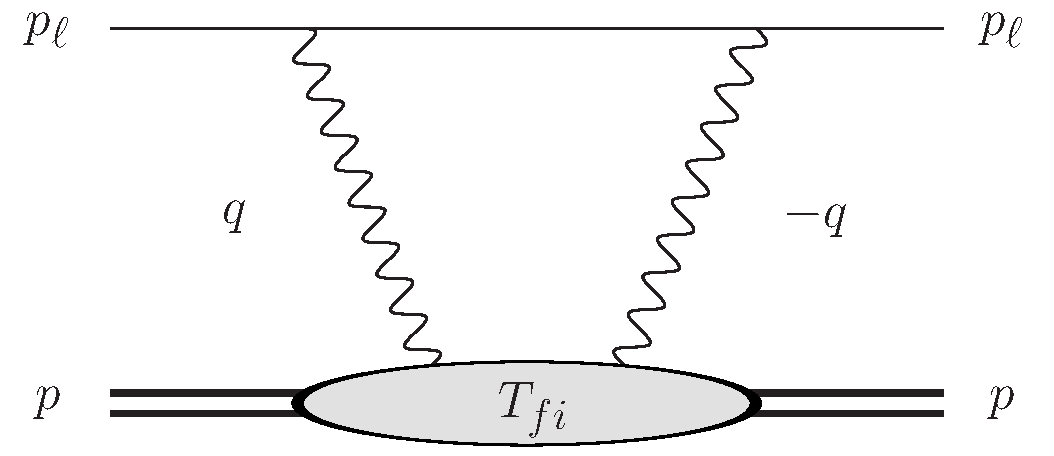
\includegraphics[width=0.4\textwidth]{figs/TPE_generic_graph.pdf}
\caption{The leading-order in $\alpha$ TPE potential. }
\end{figure}

The leading-order in $\alpha$, i.e., $O(\alpha^5)$ TPE correction to the energy of a $n\ell$ state of a muonic deuterium atom is related to the amplitude of forward doubly-virtual Compton scattering (VVCS) off an unpolarised deuteron by~\cite{Carlson:2011zd,Carlson:2013xea}
\begin{equation}
\Delta E_{n\ell}= -8i\pi \al m \,\left[\phi_{n\ell}(0)\right]^2\,
\int \!\!\frac{\dd^4 q}{(2\pi)^4}   \frac{\left(Q^2-2\nu^2\right)T_1(\nu,Q^2)-(Q^2+\nu^2)\,T_2(\nu,Q^2)}{Q^4(Q^4-4m^2\nu^2)}\,,
\label{TPE_LS}
\end{equation}
where the relevant kinematics is shown in Fig.~\ref{fig:TPE}, $Q^2=-q^2$ and $\nu = p\cdot q/M_d$ are the photon virtuality and lab frame energy, $m$ and $M_d$ are the muon and the deuteron masses, $\phi_{n\ell}(0)$ is the (Coulomb) wave function of the $n\ell$ atomic state at the origin, and $T_{1,2}(\nu,Q^2)$ are the two scalar amplitudes parametrising the unpolarised deuteron VVCS amplitude $T_{fi}$. The latter, in turn, is given by
\beq
T_{fi}=-\mathcal{E}^{'*}_\lambda\mathcal{E}^\lambda\, \epsilon^{'*}_\mu \epsilon^{\textcolor{white}{'*}}_\nu\, T^{\mu\nu}\,,
\eeq
where $\mathcal{E}$ and $\mathcal{E}^{'}$ are the polarisation vectors of the initial and final
deuteron, $\epsilon$ and $\epsilon'$ are those of the initial and final photon, and the VVCS tensor
is given by
\beq 
T^{\mu\nu} (p,q) = \left( -g^{\mu\nu}+\frac{q^{\mu}q^{\nu}}{q^2}\right)
T_1(\nu, Q^2) +\frac{1}{M_d^2} \left(p^{\mu}-\frac{p\cdot
q}{q^2}\,q^{\mu}\right) \left(p^{\nu}-\frac{p\cdot
q}{q^2}\, q^{\nu} \right) T_2(\nu, Q^2)\,.
\label{eq:VVCS_amplitude}
\eeq
Separating the amplitudes $T_{1,2}(\nu,Q^2)$ into the pole and non-pole parts, one separates the TPE correction into the elastic and non-pole part~\cite{Carlson:2013xea}. The elastic part of the TPE is readily obtained via the deuteron electromagnetic form factors. The present work only considers the non-pole part of the TPE, hence we will assume that the pole part is subtracted from the VVCS amplitude when dealing with the TPE correction.

In practice, we will use an equivalent
tensor decomposition of $T_{fi}$ in terms of the longitudinal and transverse amplitudes,
\begin{equation}
    f_L(\nu,Q^2) = -T_1(\nu,Q^2)+\left(1+\frac{\nu^2}{Q^2}\right)T_2(\nu,Q^2)\,, \qquad f_T(\nu,Q^2) = T_1(\nu,Q^2)\,.
\end{equation}
The corresponding decomposition of $T_{fi}$ takes the form
\begin{equation}
    T_{fi} = -\mathcal{E}^{'*}_\lambda\mathcal{E}^\lambda\left[\varepsilon_0\,\varepsilon_0^{\,\prime*}\,f_{L}(\nu,Q^2) +(\bv{\varepsilon} \cdot \bv{\varepsilon}^{\,\, \prime *}) \,f_{T}(\nu,Q^2)\right]\,,
\label{eq:VVCS_amplitude_LandT}
\end{equation}
where the modified polarization vector components are given by
\begin{align}
\varepsilon_0&=\left[\epsilon_0-\frac{\nu}{\left|\bv{q}\right|}\, (\bv{\epsilon}\cdot\bv{\hat q})\right]\frac{\left|\bv{q}\right|}{Q}\,,
&\bv{\varepsilon} = \bv{\epsilon}-\bv{\hat q}\,(\bv{\epsilon}\cdot\bv{\hat q})\,,\eqlab{modified_polarization_vectors}
\end{align}
with $\bv{q}$ and $\bv{\hat{q}}=\bv{q}/|\bv{q}|$ being the photon three-momentum in the lab frame and its unit vector, and $(\epsilon_0,\bv{\epsilon})$ the time and space components of the photon polarisation vector. As we will see below, the description in terms of $f_L(\nu,Q^2)$ and $f_T(\nu,Q^2)$ is natural for doing the $\slashed{\pi}$EFT counting. Both Eqs.~\eqref{eq:VVCS_amplitude} and~\eqref{eq:VVCS_amplitude_LandT} expand the amplitude in terms of gauge invariant tensors, and any other deuteron-spin independent tensors have to vanish in the sum of a gauge invariant subset of Feynman graphs. This represents an important non-trivial consistency check of our calculation, which is performed without choosing a particular electromagnetic gauge.
Note that in what follows we omit the factor 
$-\mathcal{E}^{'*}_\lambda\mathcal{E}^\lambda=\delta_{\sigma\sigma^{'}}$, where $\sigma$ and $\sigma^{'}$ are the initial and final deuteron polarisations. 

Written in terms of the longitudinal and transverse amplitudes, the TPE correction becomes
\begin{equation}
\Delta E_{n\ell}= -8i\pi \al m \,\left[\phi_{n\ell}(0)\right]^2\,
\int \!\!\frac{\dd^4 q}{(2\pi)^4}   \frac{f_L(\nu,Q^2)+2(\nu^2/Q^2)f_T(\nu,Q^2)}{Q^2(Q^4-4m^2\nu^2)}\,,
\label{eq:TPE_LT}
\end{equation}
which, after doing the Wick rotation $\nu = iq_0$ and introducing the hyperspherical coordinates, takes the form
\begin{align}
\Delta E_{n\ell}&=-
\frac{\alpha}{2\pi^2 m}\left[\phi_{n\ell}(0)\right]^2
\int \mathrm{d}^4 q
\frac{f_L(-iq_0,Q^2)-2(q_0^2/Q^2) f_T(-iq_0,Q^2)}{Q^2
\left(\frac{Q^4}{4m^2}+q_0^2\right)}\\
&=-\frac{2\alpha}{\pi m}\left[\phi_{n\ell}(0)\right]^2
\int\limits_0^\infty\frac{\mathrm{d}Q}{Q}\int\limits_{-1}^{1} \mathrm{d}x\,\sqrt{1-x^2}\,
\frac{f_L(-iQx,Q^2)-2x^2 f_T(-iQx,Q^2)}{
\frac{Q^2}{4m^2}+x^2}.
\label{eq:LS_from_LT}
\end{align}
%\subsection{Low-energy expansion}

%\subsection{Relation to two-photon-exchange correction}

\section{Pionless EFT}



\subsection{EFT expansion and counting, $Z$ parametrisation}
Here, we will briefly recap the essential details of the pionless EFT (\piEFT/) relevant for our calculation.

The pionless EFT (\piEFT/) is a theory of nucleons interacting with contact interactions~\cite{Chen:1999tn,Kaplan:1996xu,Kaplan:1998we,Kaplan:1998tg}. The high-energy scale is set by the pion mass: if the momentum transfer between two nucleons (or, broadly speaking, a typical momentum scale of the problem) is $P\ll m_\pi$, one can indeed treat a pion-exchange interaction as a contact one. The expansion is organised in powers of the ratio $P/m_\pi$. For the deuteron, the typical momentum scale is the binding momentum $\gamma\simeq 45\text{ MeV}$, resulting in an estimate of a typical expansion parameter $P/m_\pi\simeq 1/3$. To assign a particular order to a Feynman graph, one counts powers of momenta coming from the interaction vertices, propagators, and loops, assuming all momenta are of the typical size $\sim P$. Furthermore, typical energies are counted as $E\propto P^2$, which reflects the non-relativistic nature of the two-nucleon system. Correspondingly, a nucleon propagator counts as $1/E\propto P^{-2}$, whereas a loop gives a factor of $P^5$ corresponding to an integration over $d^4P=\mathrm{d}E\, \mathrm{d}^3P$.

This prescription allows one to estimate the relative importance of the longitudinal and transverse contributions to $\Delta E_{n\ell}$. The leading terms in the low-energy and low-momenta expansion of $f_L(\nu,Q^2)$ and $f_T(\nu,Q^2)$ are given by the deuteron electric and magnetic dipole polarisabilities $\alpha_{E1}$ and $\beta_{M1}$ as~\cite{Drechsel:2002ar}
\begin{align}
    f_L(\nu,Q^2) &= 4\pi \alpha_{E1}Q^2 + \dots\,,\\
    f_T(\nu,Q^2) &=-\frac{e^2}{M_d}+4\pi \beta_{M1}Q^2 + 4\pi(\alpha_{E1}+\beta_{M1})\nu^2+\dots\,,
\end{align}
where the dots denote terms at least quartic in $\nu$ and $Q$; note that the first term in the expansion of $f_T(\nu,Q^2)$ --- the Thomson term --- corresponds to the point-like deuteron and has to be subtracted when evaluating $\Delta E_{n\ell}$. The leading terms in the \piEFT/
expansion of $\alpha_{E1}$ and $\beta_{M1}$ are, respectively, $O(P^{-4})$ and $O(P^{-2})$~\cite{Chen:1998vi,Phillips:1999hh,Ji:2003ia}
\begin{align}
\alpha_{E1} &= \hpm\frac{\alpha M}{32\pi \gamma^4}+\dots\,,\\
\beta_{M1}  &= -\frac{\alpha}{32M\gamma^2}\left[
1 - \frac{16}{3}\mu_1^2 + \frac{32}{3}\mu_1^2\frac{\gamma}{\gamma_s-\gamma}
\right]+\dots\,,
\end{align}
where $M$ is the nucleon mass, $\mu_1$ is the isovector nucleon magnetic moment (in nucleon magneton units), and $\gamma_s\equiv a_s^{-1}=O(P)$ is the inverse singlet proton-neutron scattering length. Since $Q^2=\bv{q}^2-\nu^2=O(P^2)$ and $\nu^2=O(P^4)$, we can see that $f_L(\nu,Q^2)$ starts at $O(P^{-2})$, and $f_T(\nu,Q^2)$ starts two orders higher at $O(P^0)$. Furthermore, the expression for $\Delta E_{n\ell}$, Eq.~\eqref{eq:TPE_LT}, has an additional factor $\nu^2/Q^2=O(P^2)$ in front of $f_T(\nu,Q^2)$, making the transverse contribution to $\Delta E_{n\ell}$ appear first only at N4LO. 

Since we are interested in an N3LO calculation of $\Delta E_{2S}$, our aim is therefore
to calculate $f_L(\nu,Q^2)$ up to $O(P)$, or also N3LO. We will in addition also calculate $f_T(\nu,Q^2)$ up to $O(P)$, or NLO, in order to quantify the smallness of its contribution to the TPE correction, and also to investigate the (generalised) deuteron magnetic polarisability $\beta_{M1}(Q^2)$ and the deuteron generalised Baldin sum rule.

%Two-nucleon interactions start at the leading order $\propto P^{-1}$. This assignment is 

Regarding the description of the deuteron state, one can use different prescriptions to perform the expansion around the deuteron pole. Namely, the $T$ matrix in the spin-triplet (deuteron) channel is given by
\begin{align}
    T(k) = -\frac{4\pi}{M}\frac{1}{-\gamma-ik+\frac{1}{2}\rho_d(k^2+\gamma^2)+w_2(k^2+\gamma^2)^2+\dots}\,,
\end{align}
where $k$ is the $NN$ relative momentum, $\rho_d$ and $w_2$ are the deuteron effective range and shape parameter, and terms of higher-orders in $(k^2+\gamma^2)$ are not shown explicitly. This can be written as
\begin{align}
    T(k) &= -\frac{4\pi}{M}\frac{1}{\left[-\gamma-ik\right]}\frac{1}{1+\frac{1}{2}\rho_d(ik-\gamma)+w_2(ik-\gamma)(k^2+\gamma^2)+\dots}\label{eq:rhoexp}\\
    &= -\frac{4\pi}{M}\frac{1}{\left[-\gamma-ik\right]}\frac{1}{1-\gamma\rho_d+\frac{1}{2}\rho_d(ik+\gamma)+w_2(ik-\gamma)(k^2+\gamma^2)+\dots}\\
    &= -\frac{4\pi}{M}\frac{Z}{\left[-\gamma-ik\right]}\frac{1}{1+\frac{Z}{2}\rho_d(ik+\gamma)+Zw_2(ik-\gamma)(k^2+\gamma^2)+\dots}\,,\label{eq:Zexp}
\end{align}
where
\begin{align}
    Z=\frac{1}{1-\gamma\rho_d}
\end{align}
is the residue of the $T$ matrix at the deuteron pole, $k=i\gamma$. The more conventional $\rho$ expansion expands Eq.~\eqref{eq:rhoexp} in powers of small momenta and reproduces the deuteron effective range $\rho_d$ at next-to-leading order in the \piEFT/ expansion:
\begin{align}
     T(k) &= -\frac{4\pi}{M}\Bigl[
    \underbrace{\frac{1}{-\gamma-ik}}_\text{LO}
    +
    \underbrace{\frac{\rho_d}{2}\, \frac{ik-\gamma}{-\gamma-ik}}_{\text{NLO}}+\dots\Bigr]\,.
\end{align}
Alternatively, one can expand Eq.~\eqref{eq:Zexp} in powers of small momenta
and reproduce the residue at next-to-leading order in the \piEFT/ expansion:
\begin{align}
    T(k) & = -\frac{4\pi}{M}\Bigl[
    \underbrace{\frac{1}{-\gamma-ik}}_\text{LO}
    +
    \underbrace{\frac{Z-1}{-\gamma-ik}
    +\frac{Z-1}{2\gamma}}_{\text{NLO}}+\dots\Bigr]\,.
\end{align}
This scheme, called the $Z$ expansion~\cite{Phillips:1999hh}, introduces a new formal expansion parameter $(Z-1)=O(P)$. 
One can see that the leading-order $O(P^{-1})$ result  will be the same in both schemes, allowing one to reproduce the deuteron pole:
\begin{align}
    T_{-1}(k) = -\frac{4\pi}{M}\frac{1}{-\gamma-ik}\,;
\end{align}
in order to obtain it, one has to resum an infinite chain of diagrams shown in Fig.~\ref{fig:MLO}.
\begin{figure}[htb]
    \centering
    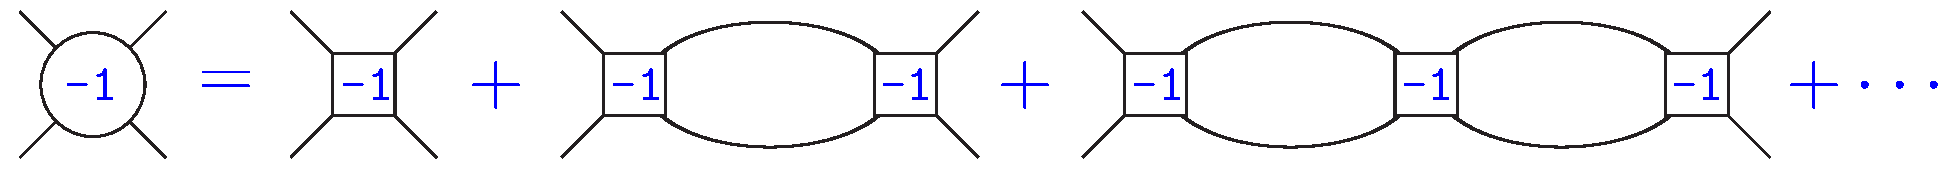
\includegraphics[width=0.85\textwidth]{figs/MLO_v1.pdf}
    \caption{The leading-order $NN$ $T$ matrix for the spin-triplet channel. Here and below, big disc (square) vertices denote insertions of a $NN$ $T$-matrix ($NN$ potential), with the number inside a vertex showing the order of the vertex in the \piEFT/ counting. The leading-order $T$ matrix in the spin-singlet ${}^1S_0$ channel is obtained analogously.}
    \label{fig:MLO}
\end{figure}
The two schemes start to differ at next-to-leading order. While the $\rho$ expansion might converge quicker if one considers, e.g., the triplet phase shifts, the $Z$ expansion reproduces the residue of the $T$ matrix at the deuteron pole already at NLO. The residue, in turn,
 is connected to the asymptotic normalisation of the deuteron $S$-wave through
 \begin{align}
 \psi(r)\to \sqrt{\frac{\gamma Z}{2\pi}}\frac{e^{-\gamma r}}{r}\,,
 \end{align}
 therefore the $Z$ expansion is better suited for quantities that receive mostly long-range contributions and are hence sensitive to the correct description of the long-range tail of the deuteron wave function~\cite{Phillips:1999hh}. As shown in that article, the deuteron electric polarisability $\alpha_{E1}$ is an example of such a long-range quantity, therefore we adopt the $Z$ expansion for our calculation.
 
% \textcolor{blue}{A remark regarding the large numerical value of the formal expansion parameter $(Z-1)=0.6876\simeq 2/3$: in practice the $Z$ expansion of an observable, e.g., an electromagnetic form factor or a VVCS amplitude, means that every contribution starting at an order $O(P^{n})$ will get multiplied by $Z=1+(Z-1)$ at order $O(P^{n+1})$. If the new contribution at $O(P^{n})$ is small, so is the corresponding $(Z-1)$ correction. --- \textit{Move to Uncertainty estimate}}

\subsection{Lagrangian and coupling constants}
The Lagrangian needed for our calculation is constructed along the usual lines formulated in, e.g, Refs.~\cite{Chen:1999tn,Kaplan:1996xu,Kaplan:1998we,Kaplan:1998tg,Chen:1999bg,Rupak:1999rk,Phillips:1999hh}, peforming a non-relativistic expansion in the one-nucleon sector and writing out the relevant two-nucleon interactions. We neglect relativistic corrections to the interactions both in the single-nucleon and in the two-nucleon sector. They count as $O(P^2/M^2)= m_\pi^2/M^2\,O(P^2/m_\pi^2)$ and are therefore more suppressed numerically than suggested by counting powers of momenta. Counting $m_\pi/M\sim P$ demotes the relativistic corrections to at least N4LO. We therefore define $\gamma=\sqrt{-M E_d}$, where $E_d=-2.224$~MeV is the deuteron energy relative to the proton and neutron at rest. We also neglect the isospin violation both due to the different proton and neutron masses and due to isospin-violating terms in the nucleon-nucleon interaction (with the caveat that the $NN$ interactions in the singlet channel are fitted to the empirical singlet $pn$ scattering length and effective range and therefore include the isospin-violating effects that are necessary to reproduce those empirical data).

 The one-nucleon Lagrangian reads
\begin{align}
\mathcal{L}^{N}&= N^\dagger\left[iD_0+\frac{\bv{D}^2}{2M}\right]N
+ \frac{e}{2M} N^\dagger \hat\mu\left(\bv\sigma\cdot\bv B \right)N + \frac{e}{6} N^\dagger\hat{r}_E^2 N\,\left(\bv{\nabla}\cdot\bv{E}\right)\,,
\label{eq:LagN}
\end{align}
with $M=M_p+M_n$ being the average nucleon mass, and $e$ the proton charge. The gauge derivatives are defined as
\begin{align}
D_0 N = \left(\partial_0 + i e \hat{Q} A_0\right) N\,,\quad \bv{D} N = \left(\bv{\nabla}-ie\hat{Q}\bv{A}\right)N
\end{align}
with $(A_0,\bv{A})$ being the electromagnetic potential, and the nucleon charge operator
\begin{align}
\hat{Q} =\frac{1}{2}(1+\tau_3)\,.
\end{align}
The electromagnetic field components are 
\begin{align}
    \bv{B} = \bv{\nabla}\times\bv{A}\,,\quad \bv{E}=-\bv{\nabla} A_0 -\partial_0\bv{A}\,,
\end{align}
and the nucleon magnetic moment and charge radius operators are defined by
\begin{align}
\hat{\mu} = \mu_0+\mu_1\,\tau_3 \,, \qquad \hat{r}^2_E= r_0^2 + r_1^2\,\tau_3\,
\end{align}
with $\mu_{0,1}=(\mu_p\pm \mu_n)/2$ and $r^2_{0,1}=(r_p^2\pm r_n^2)/2$ being the isoscalar and isovector nucleon magnetic moments (in nuclear magneton units) and charge radii, respectively.
Note that the proton charge radius contains the Foldy term $3/(4M^2)$.

Note that different parts of the minimal charge coupling are of different orders in the \piEFT/ counting: the longitudinal coupling is $\propto A_0=O(P^0)$, whereas the transverse coupling is $\propto \bv{\nabla}\cdot\bv{A}=O(P)$, and the seagull term is $\propto \bv{A}^2=O(P^0)$. Furthermore, while $\bv{B}=O(P)$, $\bv{E}$ contains two parts that are of different orders, $\bv{\nabla}A_0=O(P)$ and $\partial_0\bv{A}=O(P^2)$. The gauge invariance thus mixes different orders in the \piEFT/ counting. This is consistent with the transverse amplitude being suppressed in relation to the longitudinal one.

The Lagrangian describing $NN$ interactions in the triplet $S$-wave up to N3LO and in the singlet $S$-wave up to NLO is given by
\begin{align}
\mathcal{L}^{NN}_S&=-C_0\ N^\dagger \mathcal{P}_i N_c \ N^\dagger_c \mathcal{P}_i N
-C_0^s\ N^\dagger \mathcal{T}_a N_c \ N^\dagger_c \mathcal{T}_a N
\nonumber \\
&+
 \frac{1}{2}C_2\left[N^\dagger \mathcal{P}_i N_c\ N^\dagger_c \mathcal{O}^{(2)}_i N+ \mathrm{H.c.} 
\right]
+
 \frac{1}{2}C_2^s\left[N^\dagger \mathcal{T}_a N_c\ N^\dagger_c \mathcal{O}^{(2,s)}_a N+ \mathrm{H.c.} 
\right]
\nonumber\\
&-C_4
N^\dagger \mathcal{O}^{(2)}_i N_c
\ N^\dagger_c \mathcal{O}^{(2)}_i N
-\frac{1}{2}\tilde{C}_4\left[N^\dagger \mathcal{P}_i N_c\ N_c^\dagger \mathcal{O}^{(4)}_i N + \mathrm{H.c.}\right]
\nonumber \\\
&+\frac{1}{2}C_6\left[N^\dagger \mathcal{O}^{(2)}_i N_c\ N_c^\dagger \mathcal{O}^{(4)}_i N + \mathrm{H.c.}
\right] \,.
\label{eq:LagNN}
\end{align}
Here, we defined the charge-conjugated nucleon field as
\begin{align}
    N_c = \tau_2\,\sigma_2 \left(N^\dagger\right)^T\,;
\end{align}
note that
\begin{align}
\bv{D}N_c = \left(\bv{\nabla}+i e\hat{Q}_c \bv{A}\right)N_c
\end{align}
with
\begin{align}
    \hat{Q_c} = \tau_2\, Q\,\tau_2 = \frac{1}{2}(1-\tau_3)\,.
\end{align}
The spin-triplet, isospin-singlet and spin-singlet, isospin-triplet projectors $\mathcal{P}$ and $\mathcal{T}$ that select the corresponding $NN$ states are defined as
\begin{align}
    \mathcal{P}_i = \frac{1}{\sqrt{8}}\sigma_i\,,\qquad \mathcal{T}_a = \frac{1}{\sqrt{8}}\tau_a\,,
\end{align}
with the normalisation
\begin{align}
    \tr \mathcal{P}_i\mathcal{P}_j^\dagger = \frac{1}{2}\delta_{ij}\,, \quad  \tr \mathcal{T}_a\mathcal{T}_b^\dagger = \frac{1}{2}\delta_{ab}\,, \quad  \tr \mathcal{P}_i\mathcal{T}_b^\dagger = 0\,.
\end{align}
The quadratic and quartic Galilean-invariant combinations of the nucleon gauge derivatives and projectors are defined as
\begin{align}
\mathcal{O}_i^{(2)} &= \frac{1}{4}\left[
\overleftarrow{\bv{D}}^2\mathcal{P}_i -2 \overleftarrow{{ D}}_j\mathcal{P}_i\overrightarrow{{D}}_j + \mathcal{P}_i\overrightarrow{\bv{D}}^2
\right]
\,,
\label{eq:O2}
\\
\mathcal{O}_i^{(4)} &= \frac{1}{16}\left[
\overleftarrow{\bv{D}}^4 \mathcal{P}_i - 4\overleftarrow{\bv{D}}^2\overleftarrow{{D}}_j\mathcal{P}_i\overrightarrow{{D}}_j
+4\overleftarrow{{D}}_j\overleftarrow{{D}}_k \mathcal{P}_i \overrightarrow{{D}}_k \overrightarrow{{D}}_j +2\overleftarrow{\bv{D}}^2\mathcal{P}_i\overrightarrow{\bv{D}}^2
-4 \overleftarrow{{D}}_j\mathcal{P}_i \overrightarrow{{D}}_j\overrightarrow{\bv{D}}^2
+\mathcal{P}_i \overrightarrow{\bv{D}}^4
\right]\,
\label{eq:O4}
\end{align}
for the triplet $NN$ channel, and
\begin{align}
\mathcal{O}_i^{(2,s)} &= \frac{1}{4}\left[
\overleftarrow{\bv{D}}^2\mathcal{T}_i -2 \overleftarrow{{D}}_j\mathcal{T}_i\overrightarrow{{D}}_j + \mathcal{T}_i\overrightarrow{\bv{D}}^2
\right]
\,
\label{eq:02s}
\end{align}
for the singlet $NN$ channel. The arrows point in the direction of operation of the corresponding derivative.
Note that there is a different definition of $\mathcal{O}^{(4)}_i$ in literature, e.g., Refs.~\cite{Chen:1999bg,Rupak:1999rk} use
\begin{align}
\mathcal{O}_i^{(4)} &= \frac{1}{16}\left[
\overleftarrow{\bv{D}}^4 \mathcal{P}_i - 4\overleftarrow{\bv{D}}^2\overleftarrow{{D}}_j\mathcal{P}_i\overrightarrow{{D}}_j
+6\overleftarrow{\bv{D}}^2\mathcal{P}_i\overrightarrow{\bv{D}}^2
-4 \overleftarrow{{D}}_j\mathcal{P}_i \overrightarrow{{D}}_j\overrightarrow{\bv{D}}^2
+\mathcal{P}_i \overrightarrow{\bv{D}}^4
\right]\,.
\label{eq:O4nG}
\end{align}
The latter expression, however, is potentially problematic, because it does not produce the needed Galilean-invariant form of the matrix element:
\begin{align}
\left\langle \bv{p}_1'\, \bv{p}_2'\right|N^\dagger \mathcal{P}_i N_c\ N_c^\dagger \mathcal{O}_i^{(4)} N\left|\bv{p}_1\, \bv{p}_2\right\rangle \propto (\bv{p}_1-\bv{p}_2)^4\,.
\end{align}
Indeed, it is straightforward to see that
\begin{align}
    (\bv{p}_1-\bv{p}_2)^4 &= (\bv{p}_1^2-2\bv{p}_1\cdot\bv{p}_2+\bv{p}_2^2)^2 \nonumber\\
    & = \bv{p}_1^2-4\bv{p}_1^2\, \bv{p}_1\cdot\bv{p}_2 +4(\bv{p}_1\cdot \bv{p}_2)^2 + 2\bv{p}_1^2\bv{p}_2^2 - 4 \bv{p}_1\cdot\bv{p}_2\, \bv{p}_2^2+\bv{p}_2^4\,,
\end{align}
showing that the operator in Eq.~\eqref{eq:O4} produces the correct contractions of $\bv{p}_1$ and $\bv{p}_2$, whereas Eq.~\eqref{eq:O4nG} will produce an expression that cannot be reduced to $(\bv{p}_1-\bv{p}_2)^4$ in the general case. This issue appears to also affect the sixth-power operator $\mathcal{O}^{(6)}_i$ defined in Ref.~\cite{Rupak:1999rk} (this operator starts contributing at N4LO and is therefore not relevant for our calculation). One has to note that Eq.~\eqref{eq:O4nG} gives the correct result in the center-of-mass frame, and, since it is a relatively higher-order operator, the terms that spoil the Galilean invariance are probably rather small in a typical calculation; however, it is generally safer to use the expression given in Eq.~\eqref{eq:O4}.

The $SD$ mixing $NN$ interaction, which first appears at $O(P)$ in the $NN$ potential, is not included here, because one needs two insertions of the $SD$ mixing in order to receive a contribution to unpolarised VVCS (note also that the $SD$ interaction is proportional to the small $SD$ mixing parameter $\eta_{SD}=0.0254$). The $SD$ mixing thus starts to contribute only at $O(P^3)$ in the $NN$ potential, or N4LO.

In addition to the $S$-wave interactions, we also include the spin-triplet, isospin-triplet interactions in a $P$-wave, entering at N3LO:
\begin{align}
 \mathcal{L}^{NN}_P&=-\frac{1}{4}\left[
   C_{{}^{3\!}P_0}\delta_{ia}\delta_{jb}
 + C_{{}^{3\!}P_1}\left(\delta_{ij}\delta_{ab}-\delta_{ib}\delta_{ja}\right)
 +2C_{{}^{3\!}P_2}\left(\delta_{ij}\delta_{ab}+\delta_{ib}\delta_{ja}-\frac{2}{3}\delta_{ia}\delta_{jb}\right)
 \right] \nonumber\\
 &\times N^\dagger \mathcal{O}^{(1,P)}_{ia} N_c\ N_c^\dagger \mathcal{O}^{(1,P)}_{jb} N\,,
\end{align}
with 
\begin{align}
    \mathcal{O}^{(1,P)}_{ia} = \overleftarrow{D}_i P_a \tau_3 - \tau_3 P_a \overrightarrow{D}_i\,.
\end{align}

To complete the Lagrangian in the two-nucleon sector, one has to include two-nucleon contact interactions with the electromagnetic field whose parameters are not fixed by the $NN$ interaction. The contact terms relevant for our calculation are
\begin{align}
\mathcal{L}^{NN\gamma} & = e L_1^{M1_V} \left[N^\dagger \mathcal{P}_i N_c\ N_c^\dagger\mathcal{T}_3 N + \text{H.c.}\right]\, B_i - 2i e L_2^{M1_S}\, \epsilon_{ijk} N^\dagger \mathcal{P}_i N_c\ N_c^\dagger \mathcal{P}_j N\, B_k \nonumber\\
& - \frac{e}{2} L_1^{E1_V}\left[N^\dagger\mathcal{O}_{ij}^{(1,P)} N_c\ N_c^\dagger \mathcal{P}_j N + \text{H.c.}\right] E_i
+\frac{e}{2} L_3^{E1_V}\left[N^\dagger\mathcal{O}_{ij}^{(1,P)} N_c\ N_c^\dagger \mathcal{O}^{(2)}_j N + \text{H.c.}\right] E_i \nonumber\\
& + eL_1^{C0_S} N^\dagger\mathcal{P}_i N_c\ N_c^\dagger \mathcal{P}_i N\, \left(\bv{\nabla}\cdot\bv{E}\right)
- \frac{e}{2}L_3^{C0_S}\left[N^\dagger\mathcal{P}_i N_c\ N_c^\dagger \mathcal{O}^{(2)}_i N + \text{H.c.}\right]\, \left(\bv{\nabla}\cdot\bv{E}\right)\,.
\end{align}
The first two magnetic interactions contribute to $f_T$ at $O(P)$, or NLO, whereas the four electric contact terms contribute to $f_L$ at $O(P)$, or N3LO. Note that the convention in literature is to add to the $L_2^{M1_S}$ piece its Hermitian conjugate term, which, however, just gives the factor of $2$ that we write out explicitly.

\begin{table}[htb]
    \centering
    \begin{tabular}{c|c|c|c|c}
        $\alpha=e^2/4\pi=1/137.04$ & $\hbar c=197.326$~MeV\,fm & $M=938.27$~MeV &  $\mu_p=2.793$ & $\mu_n=-1.913$\\
         \hline 
        $r_p=0.84087$~fm & $r_n^2=-0.1161\text{ fm}^2$ & $m=105.658$~MeV & $E_d=-2.224$~MeV  & $Z=1.68758$\\
         \hline
         $w_2=0.389\text{ fm}^3$ & $\gamma_s=-8.2664$~MeV & $r_s=2.68$~fm & $C_{{}^{3\!}P_J}=-1.49\text{ fm}^4$
    \end{tabular}
    \caption{Values of single-nucleon and nucleon-nucleon parameters entering the calculation of the VVCS amplitude. \textcolor{blue}{Do we want to add any references here? Is anything missing? Do we want to use different values in the calculation? (Perhaps the value of $M$ should be changed because I define it to be the average proton and neutron mass in the text).}}
    \label{tab:couplings}
\end{table}
The coupling constants of the single-nucleon sector are well known, and we show their values in Table~\ref{tab:couplings}, which also contains the values of the $NN$ parameters used by us. The $S$-wave $NN$ coupling constants are fixed by reproducing the expansion of the $NN$ $T$ matrix in the triplet and singlet channels in \piEFT/. Throughout our calculation, we use the dimensional regularisation and the power divergence subtraction (PDS) scheme~\cite{Kaplan:1998tg,Kaplan:1998we} to regularise divergent loop integrals. This introduces a regularisation scale dependence into the calculation, for instance, the loop function that corresponds to a single loop in Fig.~\ref{fig:MLO} in this scheme is
\begin{align}
    I_0(E) & = i\int\frac{\mathrm{d}^4 l}{(2\pi)^4}\frac{1}{\left[l_0-\frac{\bv{l}^2}{2M}+i0\right]\left[E-l_0-\frac{\bv{l}^2}{2M}+i0\right]}\xrightarrow{\text{PDS}}
    -\frac{M}{4\pi}\left(\mu -\sqrt{-M E-i0}\right)\,,
\end{align}
where $E$ is the relative motion energy of the $NN$ pair, and $\mu$ the regularisation scale. The $NN$ coupling constants also depend on $\mu$ in such a way that the $T$ matrix is $\mu$-independent. Up to the order we are working at, the coupling constants are expressed in terms of $\mu$, $\gamma$, $(Z-1)$, and $w_2$ in the triplet channel, and $\mu$, $\gamma_s$, and the singlet effective range $r_s$ in the singlet channel. Note that the constants in the triplet channel are expanded in powers of the expansion parameter as well:
\begin{align}
    C_{0} = C_0^{(-1)} + C_0^{(0)} + C_0^{(1)} + C_0^{(2)} + \dots\,,
\end{align}
and analogously for the other constants. This expansion is needed in order to keep the position of the deuteron pole and the value of the residue unchanged as higher-order corrections are included. We provide the expressions for the constants entering Eq.~\eqref{eq:LagNN} below for the sake of completeness. The triplet couplings read
\begin{align}
    C_{0}^{(-1)} & = - \frac{4\pi}{M}\frac{1}{\mu-\gamma}\,,\qquad
    C_0^{(0)} =\hpm \frac{2\pi}{M}\frac{(Z-1)\gamma}{(\mu-\gamma)^2}\,,\qquad
    C_0^{(1)} =\hpm \frac{\pi}{M}\frac{(Z-1)^2\gamma(\gamma-2\mu)}{(\mu-\gamma)^3}\,,\nonumber\\
    C_0^{(2)} &=\hpm \frac{\pi}{2M}\frac{(Z-1)^3\gamma(\gamma-2\mu)^2}{(\mu-\gamma)^4}
    +\frac{4\pi}{M}\frac{w_2\gamma^4}{(\mu-\gamma)^2}    \,, \nonumber \\
    C_{2}^{(-2)} & =\hpm \frac{2\pi}{M}\frac{(Z-1)}{\gamma(\mu-\gamma)^2}\,, \qquad
    C_2^{(-1)}=-\frac{2\pi}{M}\frac{(Z-1)^2\mu}{\gamma(\mu-\gamma)^3}\,, \nonumber \\
    C_2^{(0)}&=-\frac{\pi}{2M}\frac{(Z-1)^3(\gamma^2-4\mu^2)}{\gamma(\mu-\gamma)^4}
    +\frac{8\pi}{M}\frac{w_2\gamma^2}{(\mu-\gamma)^2}   \,,\nonumber \\
    C_4^{(-3)} &= -\frac{\pi}{M}\frac{(Z-1)^2}{\gamma^2(\mu-\gamma)^3}\,, \qquad
    S_4^{(-2)} =- \frac{\pi}{2M}\frac{(Z-1)^3(\gamma-4\mu)}{\gamma^2(\mu-\gamma)^4}+\frac{4\pi}{M}\frac{w_2}{(\mu-\gamma)^2}\,, \nonumber \\
    C_6^{(-4)} &=\hpm \frac{\pi}{2M}\frac{(Z-1)^3}{\gamma^3(\mu-\gamma)^4}\,.
\end{align}
Here, $S_4^{(-2)}=C_4^{(-2)} + \tilde{C}_4^{(-2)}$ is the only linear combination of $C_4^{(-2)}$ and $\tilde{C}_4^{(-2)}$ that contributes to $NN$ scattering. We note that for the following consideration, it is convenient to eliminate the coupling $C_4^{(-2)}$, expressing it via $S_4^{(-2)}$ and $\tilde{C}_4^{(-2)}$. The LO, NLO, and N2LO couplings given here coincide with those given in Ref.~\cite{Phillips:1999hh}, however, we are not aware of any of the N3LO couplings explicitly appearing in the literature.
 Finally, the singlet couplings are
\begin{align}
 C_0^s =-\frac{4\pi}{M}\frac{1}{\mu - \gamma_s} \,, \qquad C_2^s = \frac{2\pi}{M}\frac{r_s}{(\mu-\gamma_s)^2}\,,
\end{align}
and the $P$-waves couplings contribute in a single linear combination
\begin{align}
    C_{{}^{3\!}P_J}&= C_{{}^{3\!}P_0}+2 C_{{}^{3\!}P_1}+\frac{20}{3} C_{{}^{3\!}P_2}\,,
\end{align}
whose value as extracted in Ref.~\cite{Chen:1999bg} from the Nijmegen partial wave analysis~\cite{Stoks:1993tb,Stoks:1994wp} is $-1.49\text{ fm}^4$.

The couplings of the contact terms entering $\mathcal{L}^{NN\gamma}$ cannot be inferred from the parameters of the $NN$ scattering amplitude; these contact terms, however, are crucial in compensating the $\mu$ dependence of the VVCS amplitude, and information on their couplings can be obtained from the renormalisation group equations and from processes involving external electromagnetic probes. We will discuss the role played by these contact terms as well as their determination in detail below in Sec.~\ref{sec:VVCS_results}.

%{\color{red} Check the signs of the Lagrangians --- look into the NR expansion!!!}

\section{Unpolarised VVCS in pionless EFT}
\label{sec:VVCS_results}
\subsection{LSZ reduction, expression in terms of $T$ and $\Sigma$}
In order to calculate the VVCS amplitude, we follow the LSZ reduction procedure along the lines described in, e.g., Ref.~\cite{Kaplan:1998sz} for a calculation of the deuteron electromagnetic form factors. We introduce the coupling of the $NN$ system to an interpolating deuteron field that has the appropriate quantum numbers:
\begin{align}
    \delta\mathcal{L}^{NNd}= N^\dagger \mathcal{P}_i N_c\, \mathcal{E}_i+\text{H.c.}\,, 
\end{align}
where $\mathcal{E}_i$ are the spatial components of the deuteron polarisation vector (which does not have a zeroth component in the lab frame). The VVCS amplitude is expressed via the sum of all irreducible four-point ($\gamma d\to \gamma d$) functions $\mathcal{M}(q,p,q',p')$ divided by the derivative of the deuteron self-energy $\Sigma(E)$ taken at the deuteron pole:
\begin{align}
    T_{fi} = \frac{\mathcal{M}(q,p,q',p')}{\Sigma^\prime(E_d)}\,.
    \label{eq:LSZ}
\end{align}
The irreducibility of $\mathcal{M}$ is defined in a somewhat more complicated way than in a calculation of the deuteron form factors, namely, a diagram is reducible if it contains an insertion of the LO $NN$ potential (or, equivalently, the LO $NN$ $T$ matrix) in the triplet channel at energy equal to the deuteron binding energy, i.e., at the deuteron pole. An insertion of this $T$ matrix in an off-shell kinematics is, however, allowed in an irreducible diagram. This is illustrated in Fig.~\ref{fig:reducible}.
\begin{figure}[htb]
    \centering
    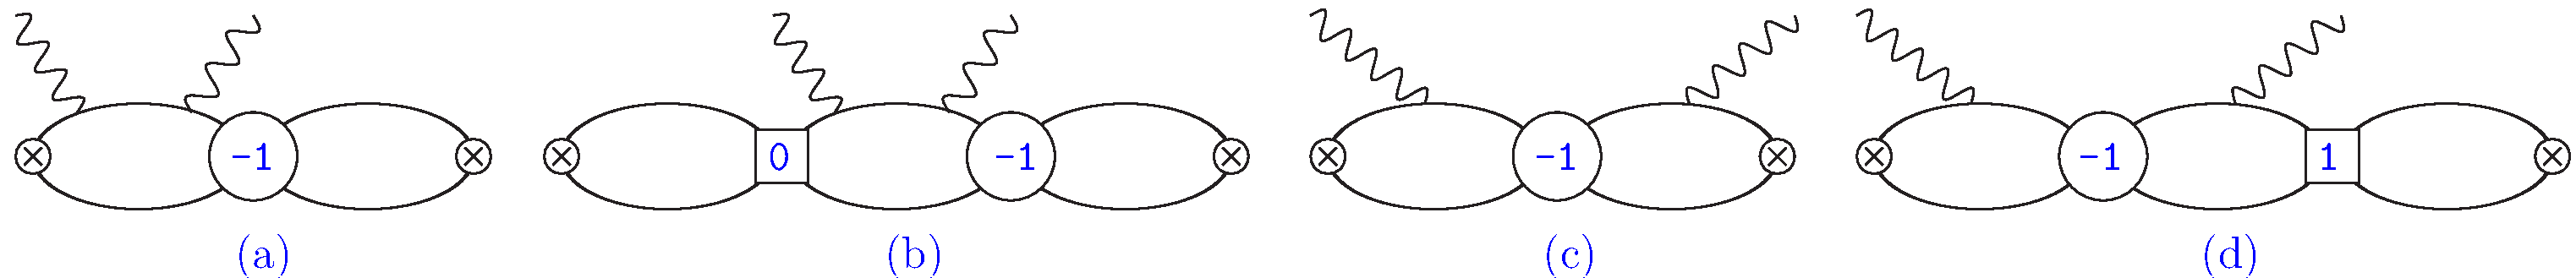
\includegraphics[width=\textwidth]{figs/reducible.pdf}
    \caption{Examples of reducible (a), (b) and irreducible (c), (d) diagrams. The crossed vertex denotes the leading-order $O(P^0)$ $NNd$ coupling.}
    \label{fig:reducible}
\end{figure}
The self energy, in turn, is defined as the sum of all deuteron-deuteron two-point functions without any insertions of the LO $NN$ $T$ matrix. 
Note that by virtue of Eq.~\eqref{eq:LSZ} the normalisation of the interpolating deuteron field in $\delta\mathcal{L}^{NNd}$ is arbitrary. To obtain the order-by-order results, both $\mathcal{M}$ and $\Sigma^\prime(E_d)$ have to be expanded, and their ratio has to be expanded after that as well:
\begin{align}
    \mathcal{M}_L(\nu,Q^2) &= \mathcal{M}_L^{(-3)}+\mathcal{M}_L^{(-2)}+\dots\,,\\
    \mathcal{M}_T(\nu,Q^2) &= \mathcal{M}_T^{(-1)}+\mathcal{M}_T^{(0)}+\dots\,,\\
    \Sigma'(E_d) & = \Sigma^{\prime(-1)}+\Sigma^{\prime(0)}+\dots\,, \\
    f_L(\nu,Q^2) & = \underbrace{\vphantom{\Bigg[}\frac{\mathcal{M}_L^{(-3)}}{\Sigma^{\prime(-1)}}}_{O(P^{-2})}+\underbrace{\vphantom{\Bigg[}\frac{\mathcal{M}_L^{(-2)}}{\Sigma^{\prime(-1)}}-\frac{\mathcal{M}_L^{(-3)}\Sigma^{\prime(0)}}{\left[\Sigma^{\prime(-1)}\right]^2}}_{O(P^{-1})}+\dots\,,\\
    f_T(\nu,Q^2) & = \underbrace{\vphantom{\Bigg[}\frac{\mathcal{M}_T^{(-1)}}{\Sigma^{\prime(-1)}}}_{O(P^{0})}+\underbrace{\vphantom{\Bigg[}\frac{\mathcal{M}_T^{(0)}}{\Sigma^{\prime(-1)}}-\frac{\mathcal{M}_T^{(-1)}\Sigma^{\prime(0)}}{\left[\Sigma^{\prime(-1)}\right]^2}}_{O(P^{1})}+\dots\,,
\end{align}
where $\mathcal{M}_{L,T}(\nu,Q^2)$ denote the terms in $\mathcal{M}$ contributing to $f_{L,T}(\nu,Q^2)$.
\subsection{Results for $\Sigma$}
To make the graphical representation of the relevant matrix elements more compact,
it is convenient to define certain subgraphs: the order-by-order corrections to the $NN$ $T$ matrix, shown in Fig.~\ref{fig:Tmatrix} and expressed via the dressed potentials that include all possible insertions of the LO NN $T$ matrix in an intermediate state, shown in Fig.~\ref{fig:V_Dressed}, and the order-by-order corrections to the $NNd$ vertex, which are shown in Fig.~\ref{fig:DeuteronVertex}. Note that the $T$ matrix always appears in full off-shell kinematics.
\begin{figure}[htb]
    \centering
    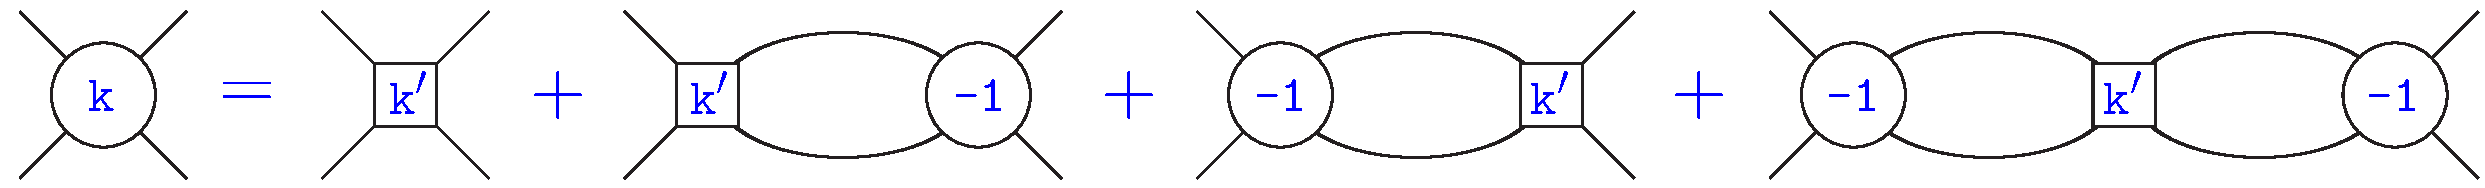
\includegraphics[width=\textwidth]{figs/M_Orders_General_v1.pdf}
    \caption{Correction to the $NN$ $T$ matrix vertex at order $k\ge 0$, defined in terms of the dressed potential at that order (denoted by the square with the primed index $k'$). Only the triplet channel is shown. The dressed potentials at the orders we are considering are shown in Fig.~\ref{fig:V_Dressed}.}
    \label{fig:Tmatrix}
\end{figure}

\begin{figure}[htb]
    \centering
    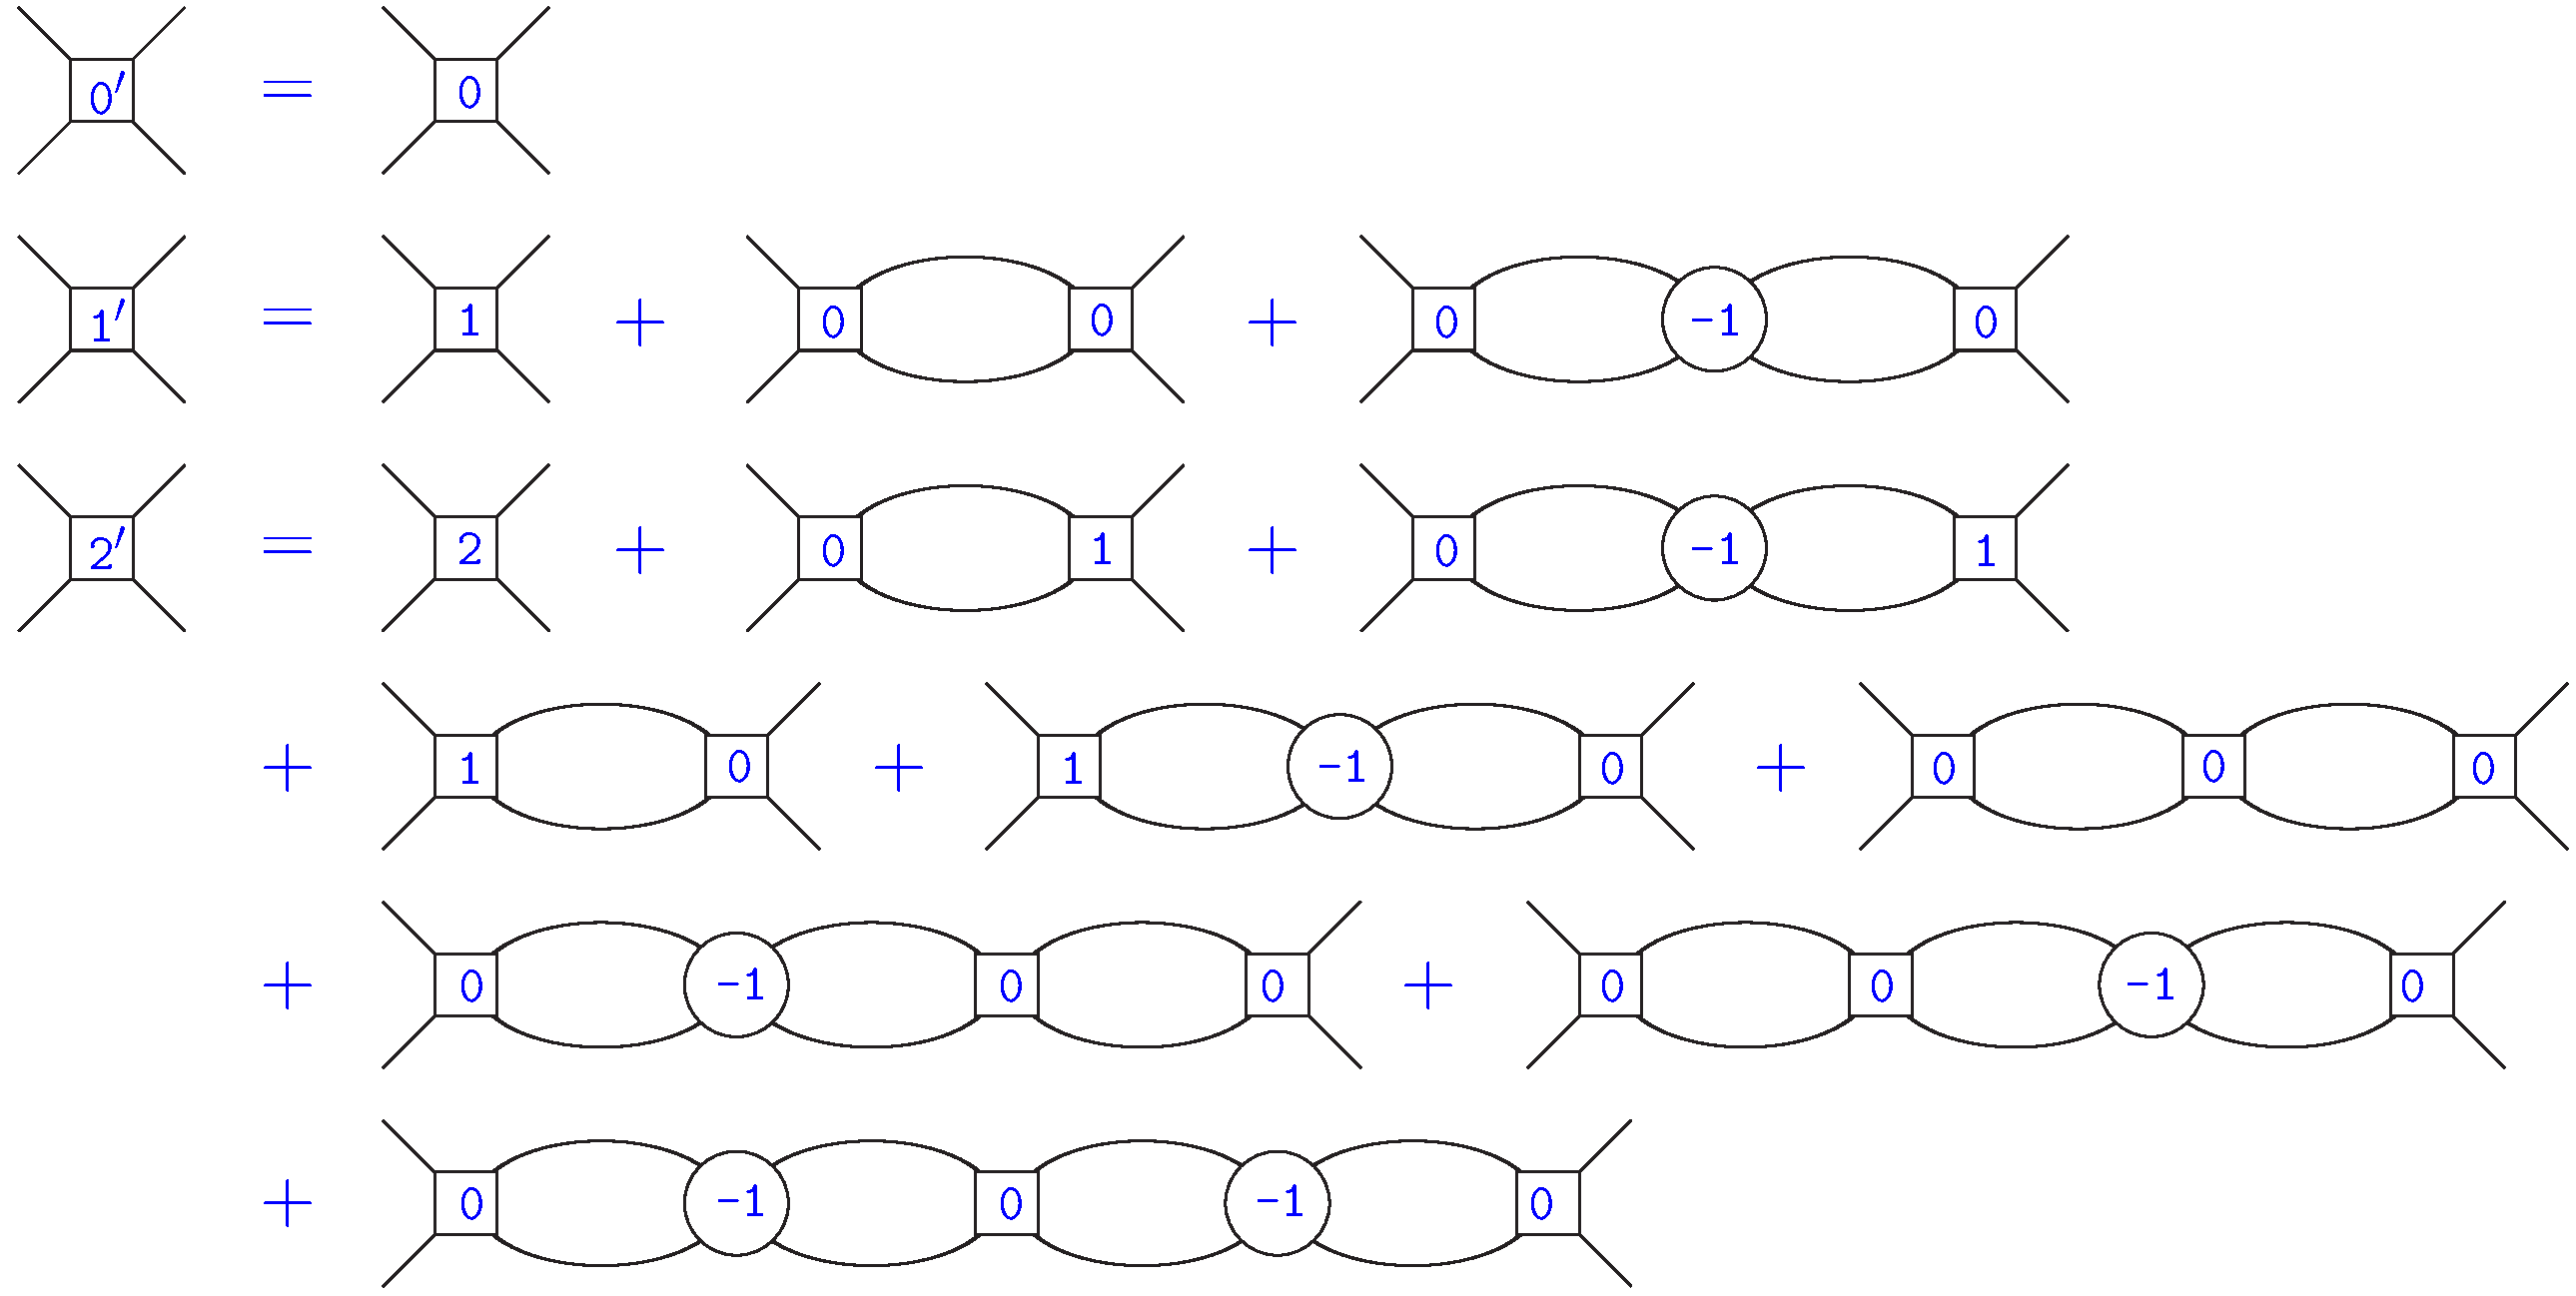
\includegraphics[width=\textwidth]{figs/V_Dressed.pdf}
    \caption{Dressed potential at $O(P^0)$, $O(P)$, and $O(P^2)$. Only the triplet channel is shown.}
    \label{fig:V_Dressed}
\end{figure}

\begin{figure}[htb]
    \centering
    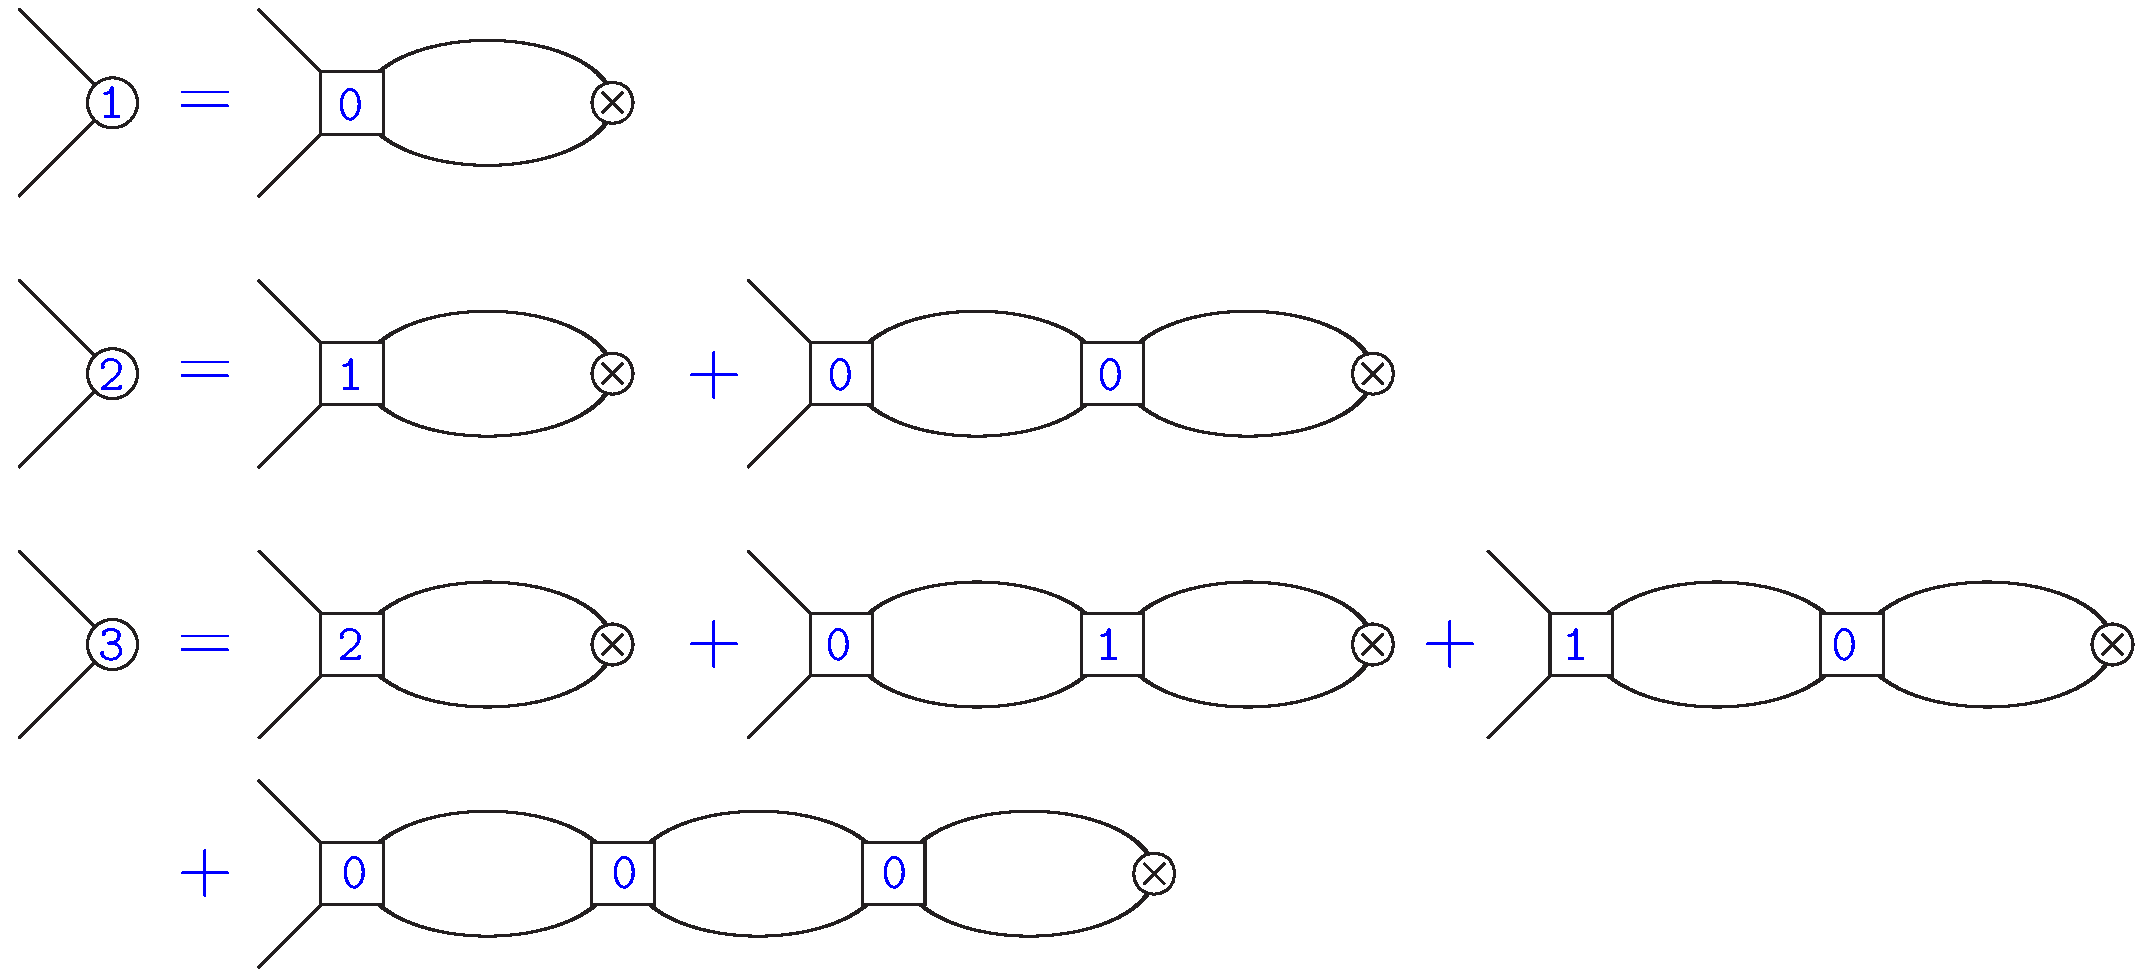
\includegraphics[width=0.82\textwidth]{figs/Deuteron_Vertex_Orders_v1.pdf}
    \caption{Corrections to the $NNd$ vertex at $O(P)$, $O(P^2)$, and $O(P^3)$, with the numbers denoting the order of the correction. Not to be confused with the $NN$ $T$ matrices defined in Figs.~\ref{fig:MLO} and~\ref{fig:Tmatrix}, which are denoted by bigger discs and have four external legs.}
    \label{fig:DeuteronVertex}
\end{figure}
With these definitions, the graphical representation for $\Sigma(E)$ takes a very compact form shown in Fig.~\ref{fig:Sigma}.
\begin{figure}[htb]
    \centering
    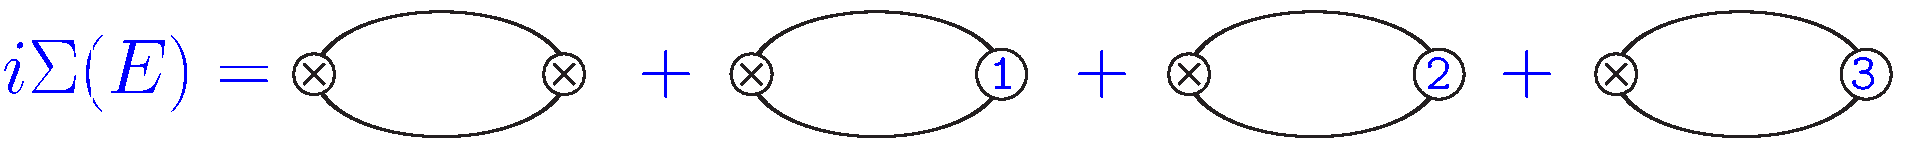
\includegraphics[width=0.78\textwidth]{figs/Sigma_Graphs_v2.pdf}
    \caption{Graphical expression for $i\Sigma(E)$ up to N3LO.}
    \label{fig:Sigma}
\end{figure}
The resulting expression for $\Sigma(E)$ up to N3LO reads
\begingroup
\allowdisplaybreaks[0]
\begin{align}
    \Sigma(E) = \frac{M}{4\pi}&\Bigg[\mu + ik \nonumber \\
    &+\frac{(Z-1) \left(\gamma ^2+k^2\right) (k-i \mu )^2}{2 \gamma  (\gamma -\mu )^2}\nonumber \\
    &+\frac{(Z-1)^2 \left(\gamma ^2+k^2\right) (\mu +i k)^2 \left(\gamma  \left(\gamma ^2-2 \gamma  \mu +2 \mu ^2\right)+i k^3-k^2 (\gamma -2 \mu )+i \gamma ^2 k\right)}{4 \gamma ^2 (\gamma -\mu )^4}\nonumber\\
    &-\frac{(Z-1)^3 \left(\gamma ^2+k^2\right) (k-i \mu )^2 \left(-i \gamma  \left(\gamma ^2-2 \gamma  \mu +2 \mu ^2\right)+k^3+i k^2 (\gamma -2 \mu
   )+\gamma ^2 k\right)^2}{8 \gamma ^3 (\gamma -\mu )^6}\nonumber\\
   &+\frac{w_2 \left(\gamma ^2+k^2\right)^2 (k-i \mu )^2}{(\gamma -\mu )^2}+\dots
    \Bigg]\,,
\end{align}
\endgroup
where $k=i\sqrt{-ME}$, and the N3LO result occupies the last two lines. Even though $\Sigma(E)$ depends on $\mu$, its derivative at the deuteron pole, $\Sigma^\prime(E_d)$, is $\mu$-independent, and the order-by-order expression for it is very compact:
\begin{align}
\Sigma^\prime(E_d) &= \frac{M^2}{8\pi\gamma}\left[1-(Z-1)+(Z-1)^2-(Z-1)^3+\dots\right]\,,
\end{align}
giving an even simpler expression for the inverse quantity:
\begin{align}
    \left[\Sigma^\prime(E_d)\right]^{-1} & = \frac{8\pi\gamma}{M^2}\left[1+(Z-1)+0+0+\dots\right]\,.
\end{align}

\subsection{Results for $\mathcal{M}$}
\subsubsection{LO}
\begin{figure}[htb]
    \centering
    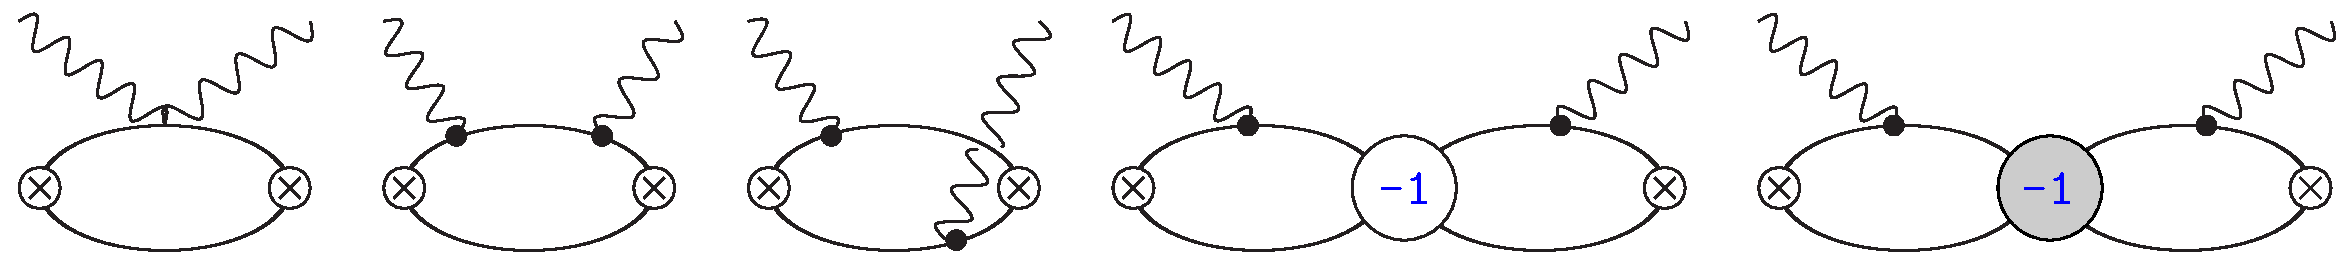
\includegraphics[width=\textwidth]{figs/VVCS_LO.pdf}
    \caption{Diagrams contributing to $i\mathcal{M}$ at LO, i.e., $O(P^{-3})$ for $\mathcal{M}_L$ and $O(P^{-1})$ for $\mathcal{M}_T$. Dotted vertices are the sum of the charge and the magnetic moment couplings from the single-nucleon Lagrangian; the big grey disc denotes the LO $NN$ $T$ matrix in the singlet channel. Crossed graphs are not shown.}
    \label{fig:LO}
\end{figure}
Here, we will show the results for the four-point function $\mathcal{M}$. The diagrams contributing to $i\mathcal{M}$ at LO are shown in Fig.~\ref{fig:LO}, resulting in
\begin{align}
\mathcal{M}_{L}^{(-3)} & = \frac{e^2M^3}{\pi}\frac{Q^2}{\bv{q}^2}\left[\frac{1}{2 \gamma  \left[\bv{q}^2+4 (\gamma +\lambda_d)^2\right]}-\frac{\phi^2(\nu,\bv{q}^2)}{\bv{q}^2 (\gamma-\lambda_d)}\right]+(\nu\to-\nu)\,,\\
\mathcal{M}_{T}^{(-1)} = \frac{e^2M}{\pi}\Bigg[& -\frac{16\gamma  (\gamma -\lambda_d) (\gamma +\lambda_d)^2+4 \bv{q}^2 \left(2 \gamma ^2+\gamma  \lambda_d+\lambda_d^2\right)-\left(4 \mu_1^2+4 \mu_0^2-1\right)\bv{q}^4 }{16 \gamma\,  \bv{q}^2
   \left[\bv{q}^2+4 (\gamma +\lambda_d)^2\right]}\nonumber\\
   &+
 \left(\frac{|\bv{q}| (\mu_0^2-\mu_1^2)}{12 M\nu}+\frac{4 \gamma ^2-4 \lambda_d^2+\bv{q}^2}{8 |\bv{q}|^3}\right)\phi(\nu,\bv{q}^2)\nonumber\\
  &
-\frac{1}{3} \left(\frac{2 \mu_0^2}{\gamma-\lambda_d}
+\frac{\mu_1^2}{\gamma_s-\lambda_d}\right)\phi^2(\nu,\bv{q}^2)
   \Bigg]+(\nu\to-\nu)\,,
\label{eq:MLO}
\end{align}
where the kinematic functions are defined as
\begin{equation}
\lambda_d=\sqrt{\gamma^2-M\nu+\frac{\bv{q}^2}{4}}\,,\qquad \phi(\nu,\bv{q}^2)=\arctan\frac{\left|\bv{q}\right|}{2(\gamma+\lambda_d)}\,.
\end{equation}
These expressions (as well as those at higher orders shown below) include the pole parts, with the elastic poles shifted due to the non-relativistic expansion and located at $\nu=\pm\bv{q}^2/(4M)$. One can also note that all loop integrals at LO are convergent, so no $\mu$ dependence emerges at this step.

\subsubsection{NLO}
The NLO contributions to $\mathcal{M}$ come from diagrams shown in Figs.~\ref{fig:NLO} and~\ref{fig:NLO_CT}.
\begin{figure}[htb]
    \centering
    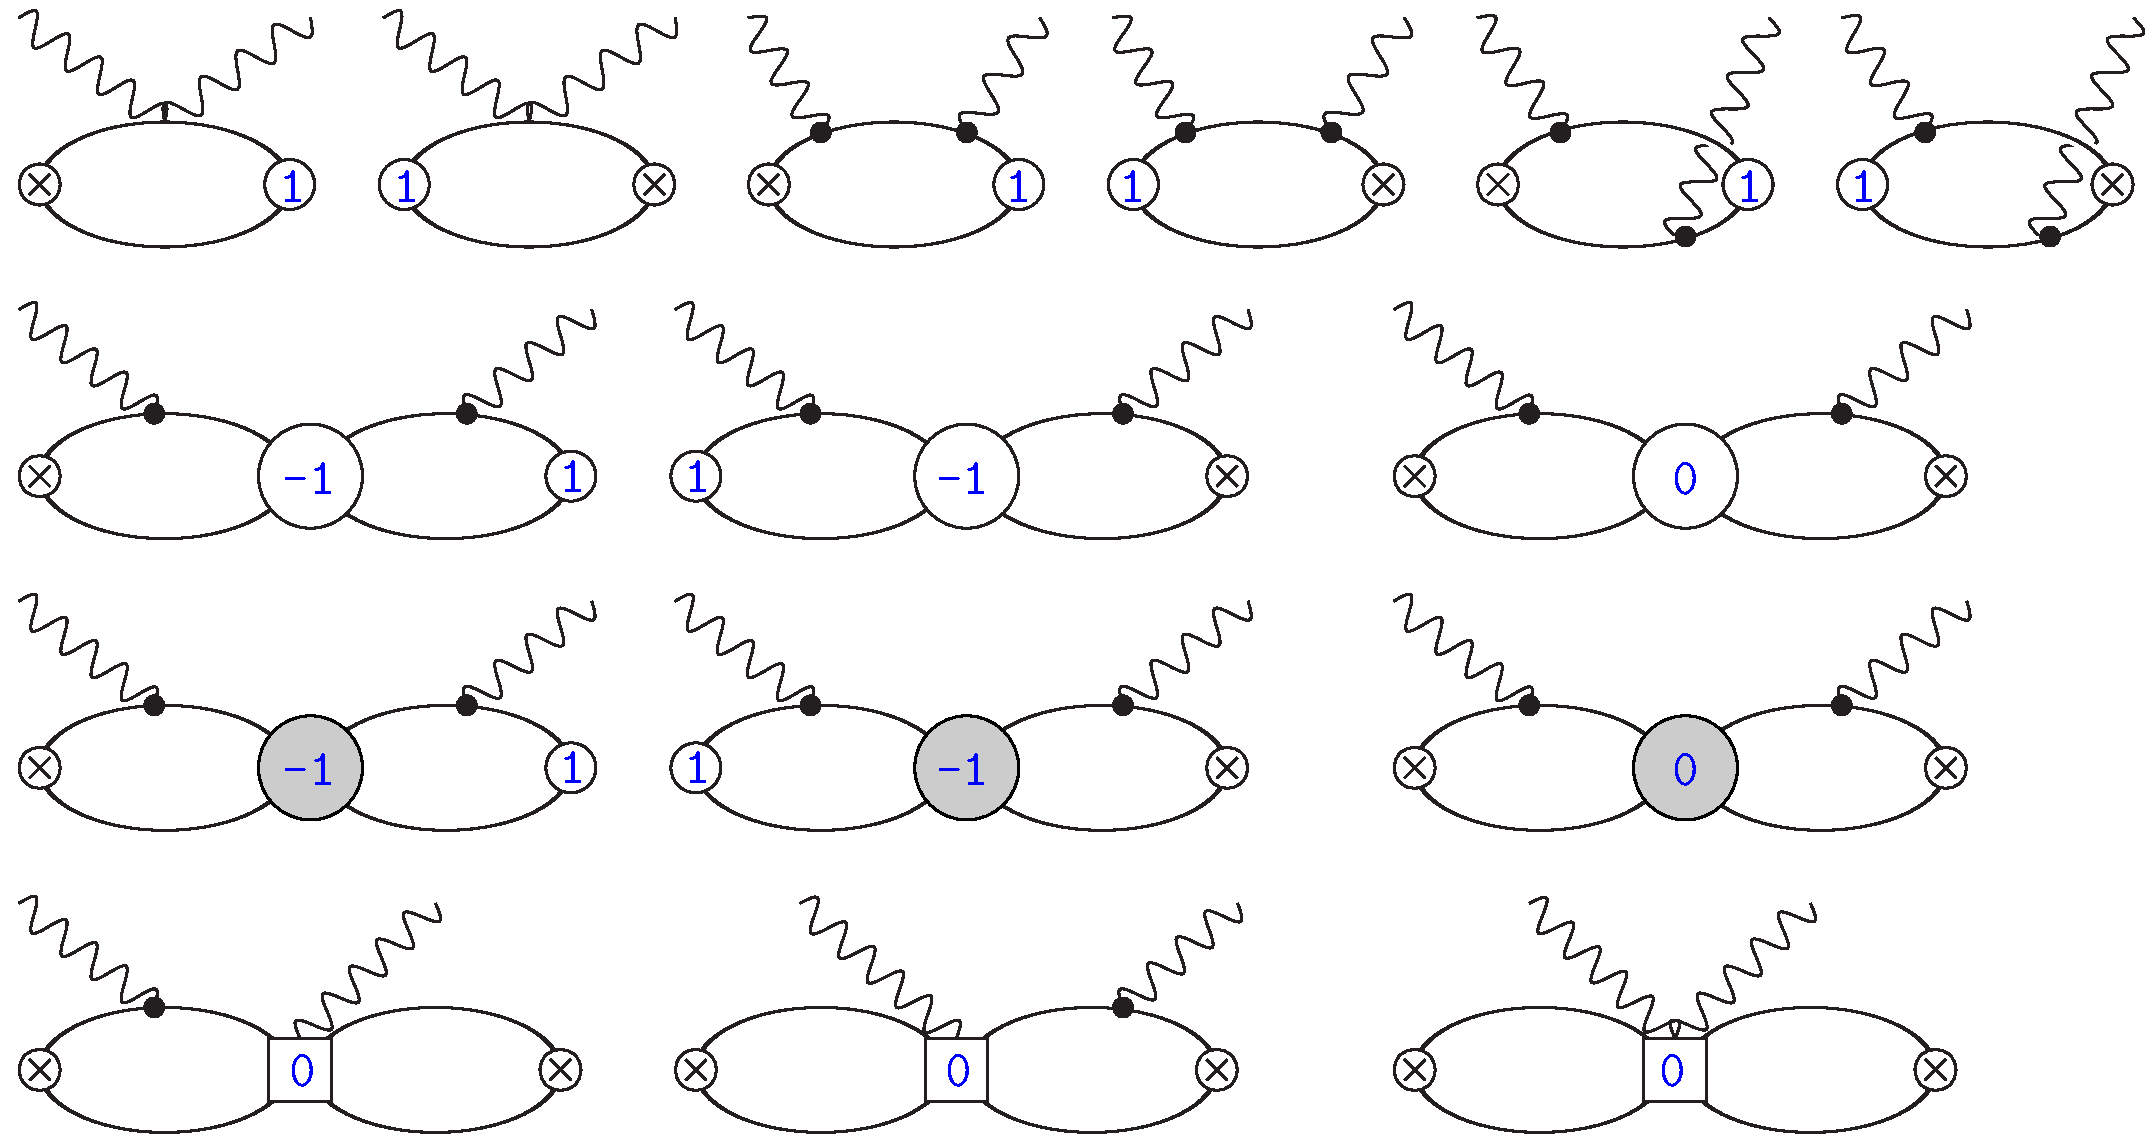
\includegraphics[width=\textwidth]{figs/VVCS_NLO.pdf}
    \caption{Contributions to $i\mathcal{M}$ at NLO, i.e., $O(P^{-2})$ for $\mathcal{M}_L$ and $O(P^0)$ for $\mathcal{M}_T$, due to NLO corrections in the $NN$ interaction. The notation is as in Fig.~\ref{fig:LO}. Crossed graphs are not shown.}
    \label{fig:NLO}
\end{figure}
While the contributions to $\mathcal{M}_{L}^{(-2)}$ only come from the graphs in Fig.~\ref{fig:NLO}, and their sum is $\mu$ independent, $\mathcal{M}_{T}^{(0)}$ also receives contributions from the
two magnetic contact terms in $\mathcal{L}^{NN\gamma}$, corresponding to graphs in Fig.~\ref{fig:NLO_CT}. 
\begin{figure}[htb]
    \centering
    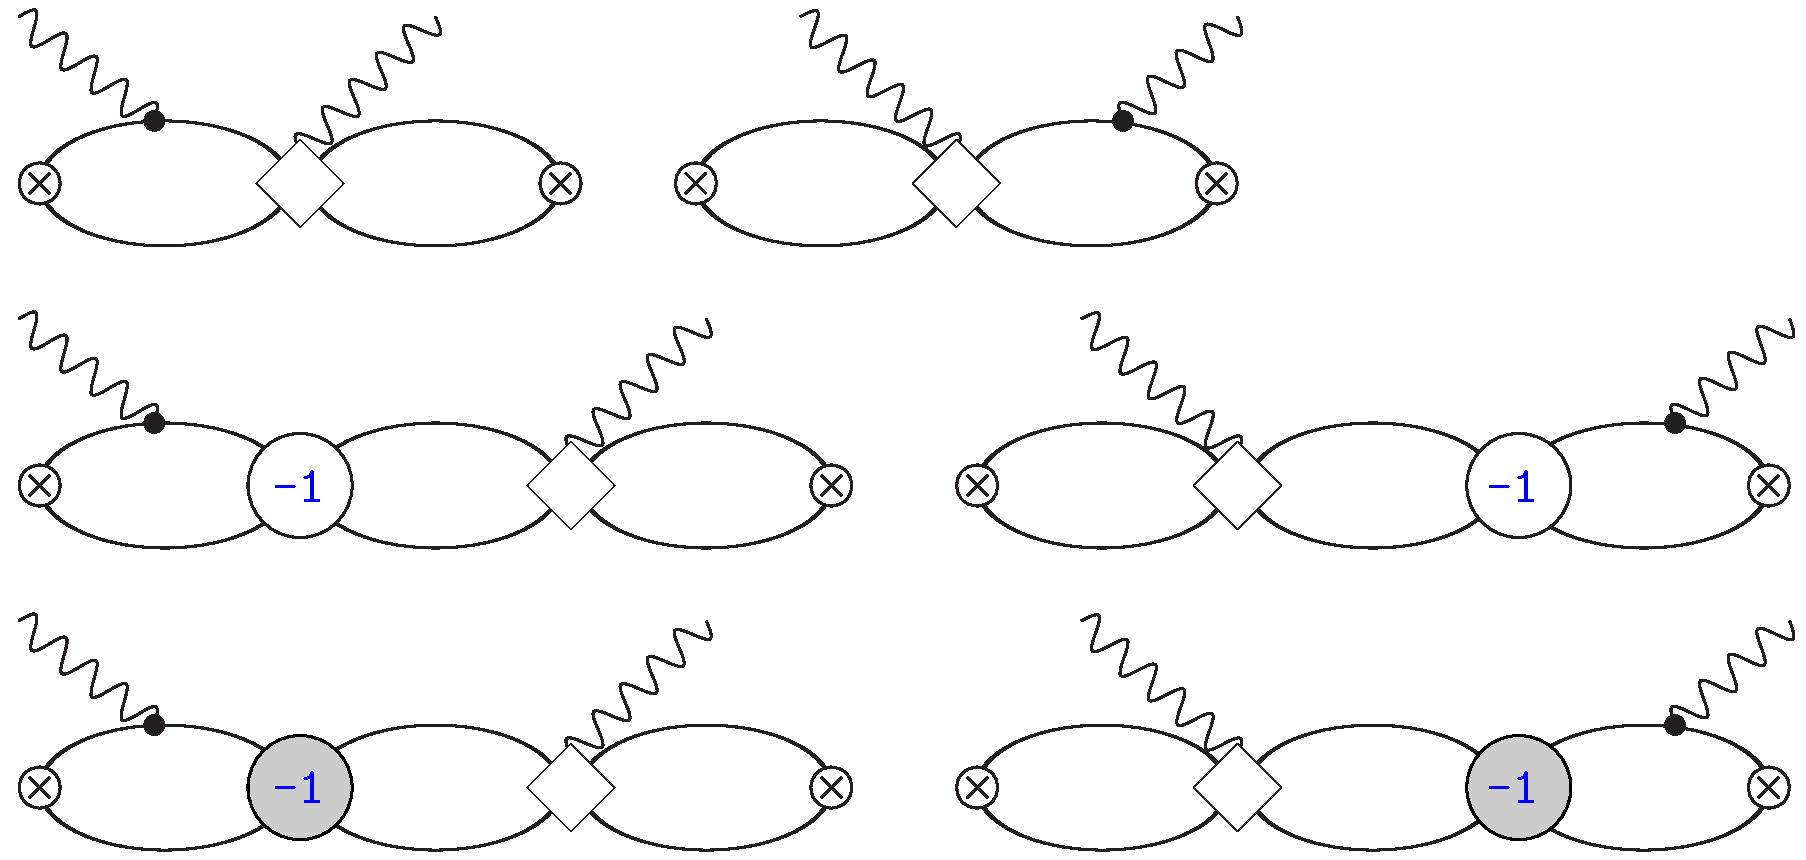
\includegraphics[width=0.8\textwidth]{figs/VVCS_NLO_CT.pdf}
    \caption{Contributions to $i\mathcal{M}$ at NLO due to the magnetic contact terms $L_1^{M1_V}$ and $L_2^{M1_S}$ (shown as diamonds). The rest of the notation is as in Fig.~\ref{fig:LO}. These graphs give an $O(P^0)$ contribution to $\mathcal{M}_T$ only. Crossed graphs are not shown.}
    \label{fig:NLO_CT}
\end{figure}
The renormalisation scale dependence of the coupling constants $L_1^{M1_V}$ and $L_2^{M1_S}$ has to cancel out the $\mu$ dependence of the total NLO contribution to $\mathcal{M}_{T}$. We find the following RG equations for these two couplings:
\begin{align}
\mu\frac{\mathrm{d}\hphantom{\mu}}{\mathrm{d}\mu}\left[(\mu-\gamma)(\mu-\gamma_s)\left(L_1^{M1_V}-\frac{\mu_1}{2}\left\{C_2^{(-2)}+C_2^{(-2,s)}\right\}\right)\right] & = 0\,,
\label{eq:RG_magnetic_1}
\\
\mu\frac{\mathrm{d}\hphantom{\mu}}{\mathrm{d}\mu}\left[\frac{L_2^{M1_S}}{C_2^{(-2)}}\right] & = 0\,.
\label{eq:RG_magnetic_2}
\end{align}
This is consistent with the results obtained in Refs.~\cite{Chen:1999bg,Rupak:1999rk,Ji:2003ia}. The first of these coupling constants, $L_1^{M1_V}$, contributes to the deuteron $\beta_{M1}$. The value of the RG-invariant quantity in Eq.~\eqref{eq:RG_magnetic_1} can be fitted to, e.g., data on $np\to d\gamma$; we will use the result from Ref.~\cite{Rupak:1999rk} that found, also in the $Z$ expansion,
\begin{equation}
(\mu-\gamma)(\mu-\gamma_s)\left(L_1^{M1_V}-\frac{\mu_1}{2}\left\{C_2^{(-2)}+C_2^{(-2,s)}\right\}\right) =-9.039(27)\text{ fm}^2\,.
%-9.039\pm 0.027\text{ fm}^2\,.
\label{eq:L1M_value}
\end{equation}
The value of $L_2^{M1_S}$ is fitted to the deuteron magnetic moment, obtaining~\cite{Kaplan:1998sz,Chen:1999tn}
\begin{equation}
L_2^{M1_S}\Big|_{\mu=m_\pi}=-0.149\text{ fm}^4\,;
\label{eq:L2M_value}
\end{equation}
this result is the same  at NLO both in the $Z$ and in the $\rho$ expansion.
To make the expression for $\mathcal{M}_T^{(0)}$ more compact, we introduce dimensionless $\mu$-independent couplings $l_1^{M1_V}$ and $l_2^{M1_S}$ according to
\begin{align}
L_1 & = \frac{\mu_1}{2}\left(C_2^{(-2)}+C_2^{(-2,s)}\right)+\frac{\pi (Z-1)}{M\gamma}\frac{l_1^{M1_V}}{(\mu-\gamma)(\mu-\gamma_s)}\,,\\
L_2 & = l_2^{M1_S}\, C_2^{(-2)}\,.
\end{align}
The resulting expressions for $\mathcal{M}_L$ and $\mathcal{M}_T$ read
\begin{align}
    \mathcal{M}_L^{(-2)} & =\frac{e^2 M^3}{\pi}\frac{Q^2}{\bv{q}^2} \frac{(Z-1)}{2\gamma}\frac{ \phi(\nu,\bv{q}^2) \left[|\bv{q}|-(\gamma +\lambda_d) \phi(\nu,\bv{q}^2)\right]}{ \bv{q}^2 (\gamma -\lambda_d)}+(\nu\to-\nu)\,,\\
    \mathcal{M}_T^{(0)}  = \frac{e^2 M}{\pi}\Bigg[&
    \frac{Z-1}{32 \gamma }
    -\frac{(Z-1)}{12\gamma}|\bv{q}|
    \left(
    \frac{\mu_1\,l_1^{M1_V} }{\gamma_s-\lambda_d}-\frac{4 \mu_0(\mu_0-2l_2^{M1_S})}{\gamma-\lambda_d}
    \right)\phi(\nu,\bv{q}^2)\nonumber\\
    &+\frac{1}{6} 
    \left(
    \frac{ \mu_1^2\, r_s\,\lambda_d^2}{(\gamma_s-\lambda_d)^2}-\frac{2 (Z-1) \mu_0^2 (\gamma +\lambda_d)}{\gamma  (\gamma -\lambda_d)}
    \right)\phi^2(\nu,\bv{q}^2)
   \Bigg]+(\nu\to-\nu)\,.
\end{align}
The values of the coupling constants $l_1^{M1_V}$ and $l_2^{M1_S}$, obtained using the values in Eqs.~\eqref{eq:L1M_value} and~\eqref{eq:L2M_value}, are
\begin{align}
l_1^{M1_V} = -4.603(14) \,,\qquad l_2^{M1_S} = -8.59\times 10^{-3}\,.
\label{eq:l1M_l2M_value}
\end{align}
While $l_1^{M1_V}$ could be considered as being of a natural size, $l_2^{M1_S}$ is numerically small due to the LO contribution already coming very close to the empirical value of the deuteron magnetic moment, as pointed out in Refs.~\cite{Kaplan:1998sz,Chen:1999tn}.
\subsubsection{NNLO}
From this point on, we only keep track of those interactions that contribute to $f_L$, and, as a check, also include contributions to $\mathcal{M}$ that are needed to satisfy the electromagnetic gauge invariance. In practice this means taking into account the minimal coupling, both in the single-nucleon and in the two-nucleon Lagrangian. Incidentally, this allows one to also check that the Thomson term is recovered at NNLO and NNNLO.
The corresponding diagrams that appear at NNLO are shown in Figs.~\ref{fig:NNLO} and~\ref{fig:NNLO_RE}.
\begin{figure}[htb]
    \centering
    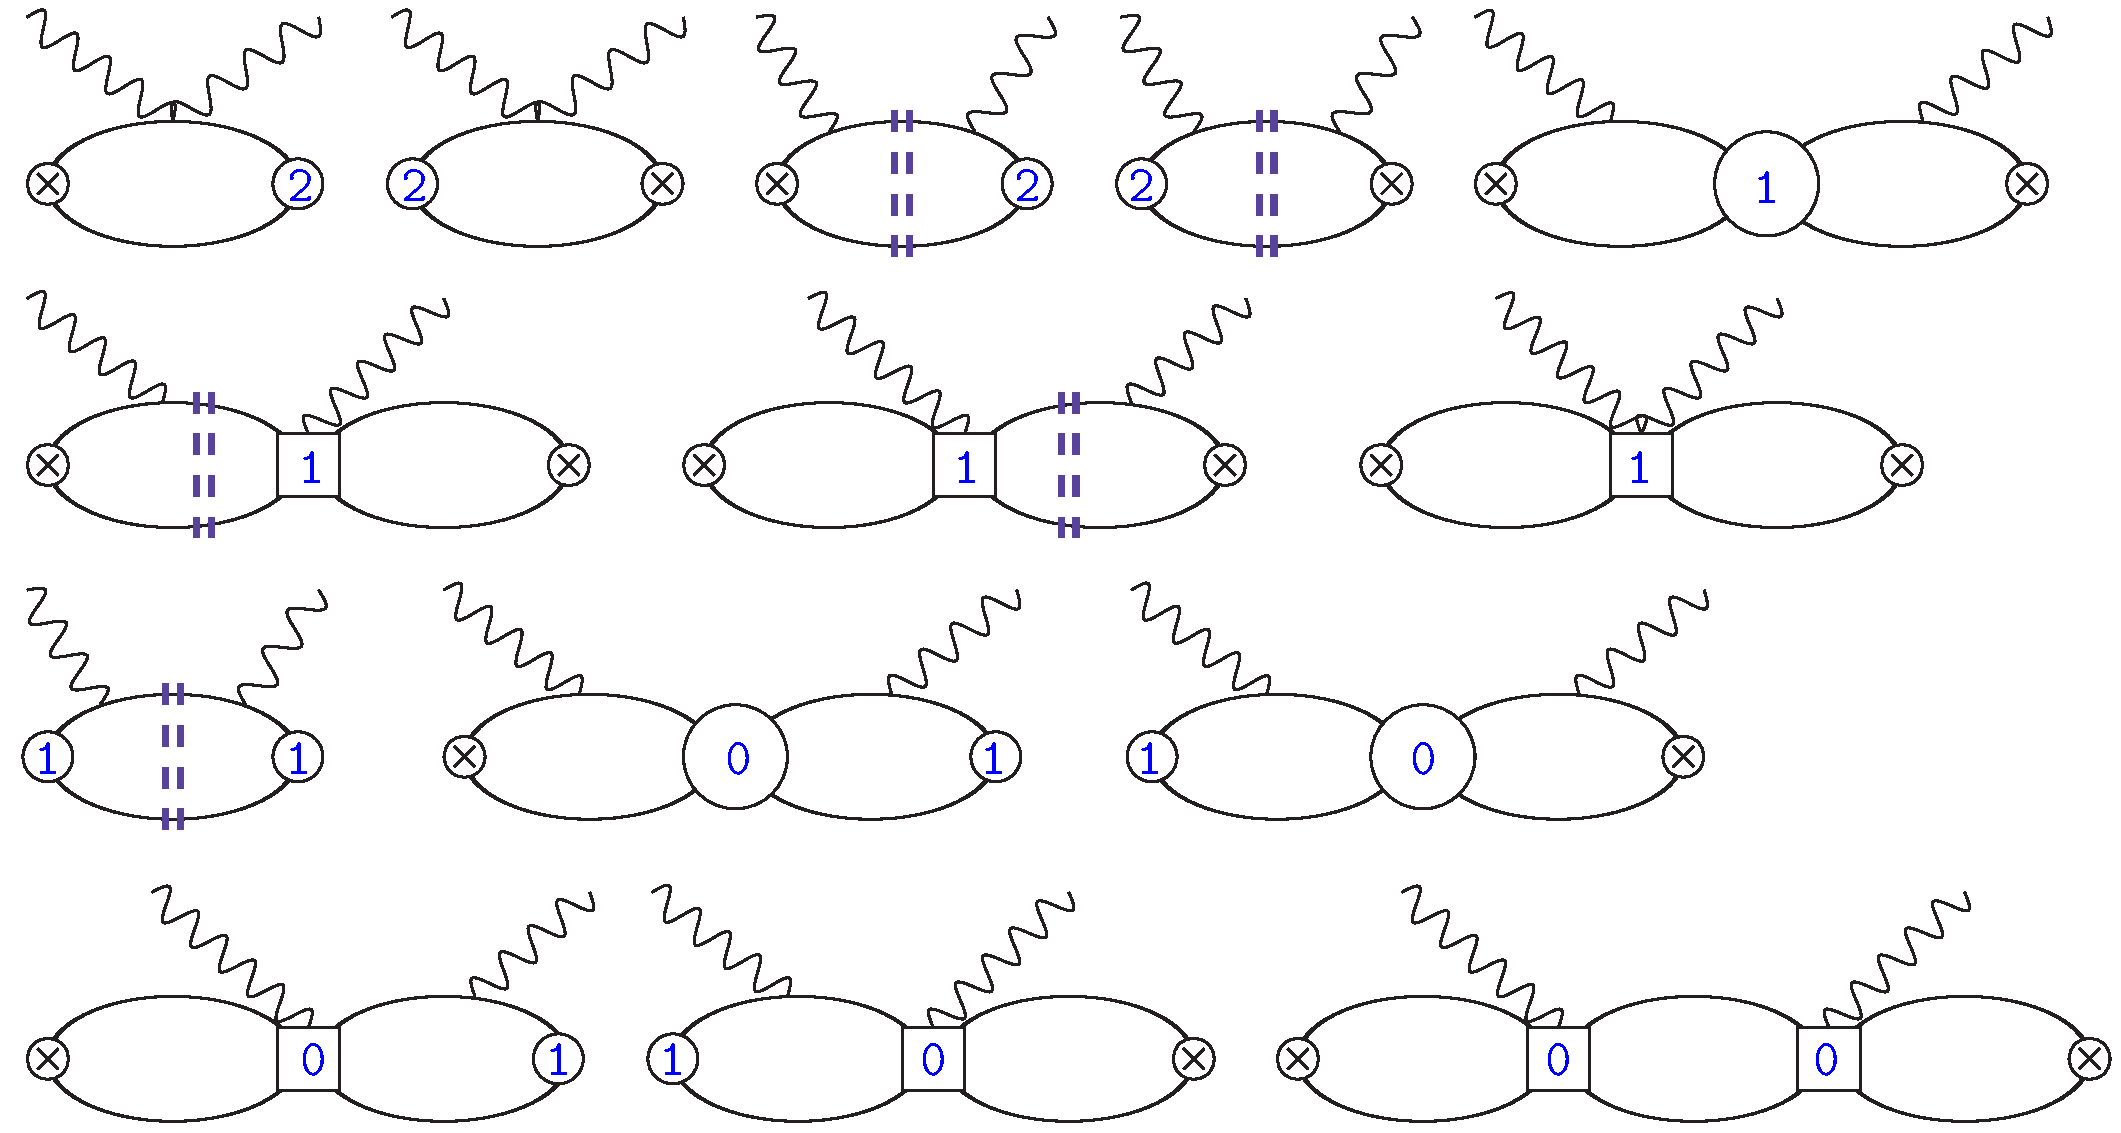
\includegraphics[width=\textwidth]{figs/VVCS_NNLO.pdf}
    \caption{Diagrams that contribute to $\mathcal{M}_L$ at NNLO, i.e., $O(P^{-1})$, due to NNLO terms in the $NN$ interaction. The nucleon-photon vertex is exclusively the minimal coupling. In addition to diagrams that actually contribute to $f_L$, we also show those that are necessary in order to keep the electromagnetic gauge invariance. The vertical double dashed lines indicate possible insertions of a LO $NN$ $T$ matrix in the spin-triplet channel. Crossed graphs are not shown.}
    \label{fig:NNLO}
\end{figure}
At this order, one is still getting a $\mu$-independent contribution to $\mathcal{M}_L$ from loops with NNLO corrections to $NN$ interactions, Fig.~\ref{fig:NNLO}.
\begin{figure}[htb]
    \centering
    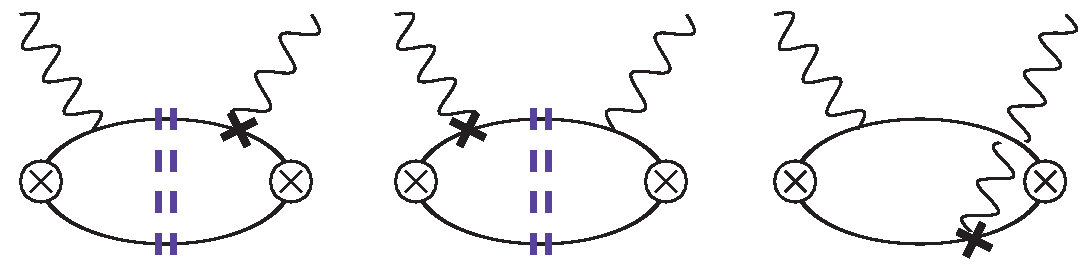
\includegraphics[width=0.5\textwidth]{figs/VVCS_NNLO_RENucl.pdf}
    \caption{Correction to $i\mathcal{M}_L$ due to the photon coupling proportional to $\hat{r}^2$, denoted by the black cross vertex, contributing at $O(P^{-1})$. The rest of the notation is as in Fig.~\ref{fig:NNLO}. Crossed graphs are not shown.}
    \label{fig:NNLO_RE}
\end{figure}
The resulting contribution to the longitudinal part of the four-point function is
 \begin{align}
\mathcal{M}_{L}^{(-1)} & =\frac{e^2M^3}{\pi}\frac{Q^2}{\bv{q}^2}\frac{(Z-1)^2}{4\gamma^2}
\left[-\frac{1}{4(\gamma -\lambda_d)}-\frac{ \phi(\nu,\bv{q}^2)}{|\bv{q}|}+
\frac{(\gamma +\lambda_d) \phi^2(\nu,\bv{q}^2)}{\bv{q}^2}
\right]+(\nu\to-\nu)\,.
 \end{align}
 In addition, there are the corrections due to the nucleon charge radius operator, shown in Fig.~\ref{fig:NNLO_RE}. Their contribution is
\begin{align}
\delta\mathcal{M}_{L}^{(-1)}  = -\frac{e^2 M^3}{6\pi}\frac{Q^2}{\bv{q}^2}\biggl[&\frac{(r_0^2+r_1^2)\bv{q}^2 }{\gamma
\left[\bv{q}^2+4 (\gamma +\lambda_d )^2\right]}+
\frac{(r_0^2-r_1^2)|\bv{q}|  \phi(\nu,\bv{q}^2)}{M \nu }\nonumber\\
&-\frac{4 r_0^2\, 
\phi^2(\nu,\bv{q}^2)}{\gamma -\lambda_d}\biggr]+(\nu\to-\nu)\,.
\end{align}


 
\subsubsection{NNNLO}
Finally, the NNNLO contribution to $\mathcal{M}_L$ comes from three types of diagrams: those with insertions of the NNNLO $NN$ interactions, shown in Fig.~\ref{fig:NNNLO}, diagrams with an insertion of a gauge-invariant electric contact term, shown in Fig.~\ref{fig:NNNLO_CT}, and corrections generated by one insertion of the nucleon charge radii coupling in the NLO graphs, as shown in Fig.~\ref{fig:NNNLO_RE}.
\begin{figure}[!htbp]
    \centering
    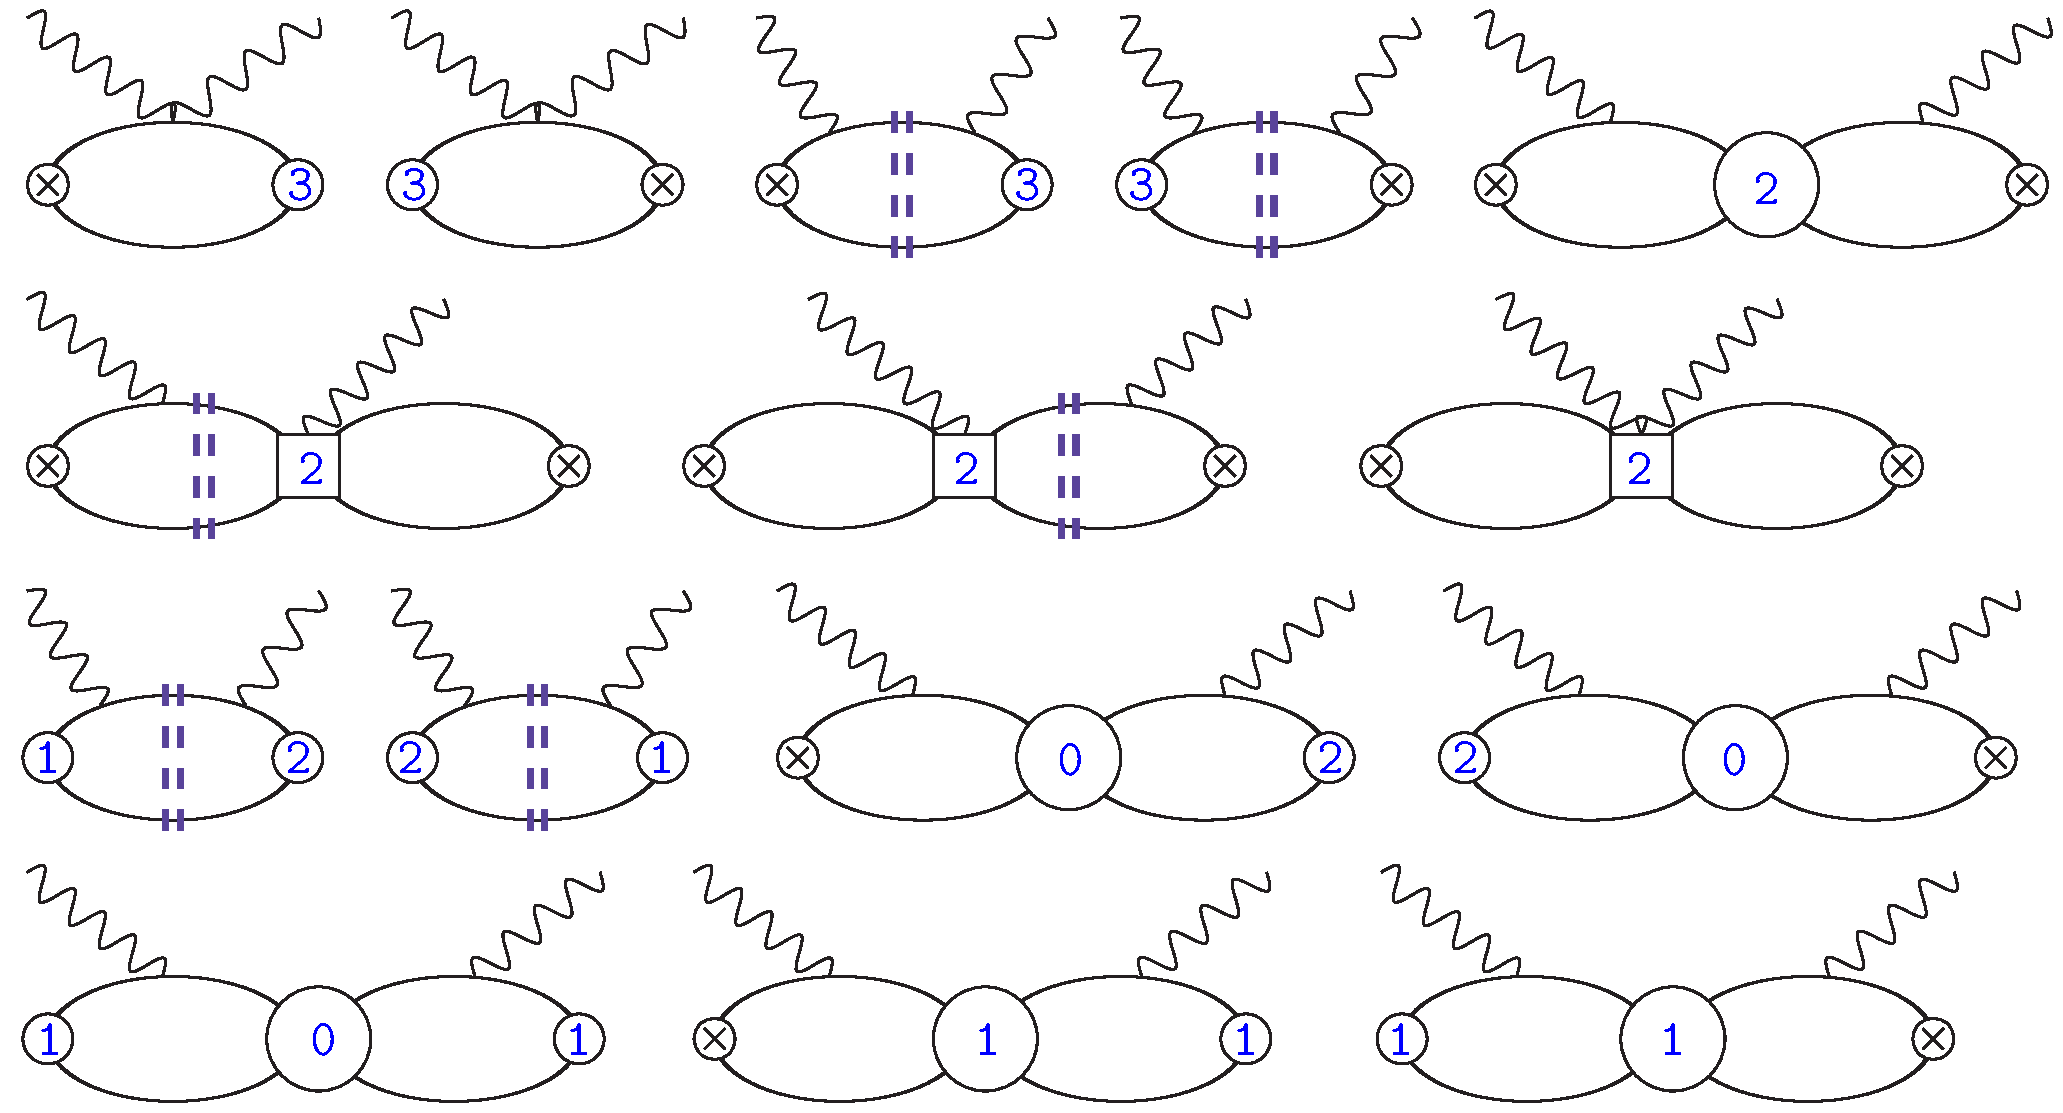
\includegraphics[width=0.98\textwidth]{figs/VVCS_NNNLO_v1.pdf}\\
     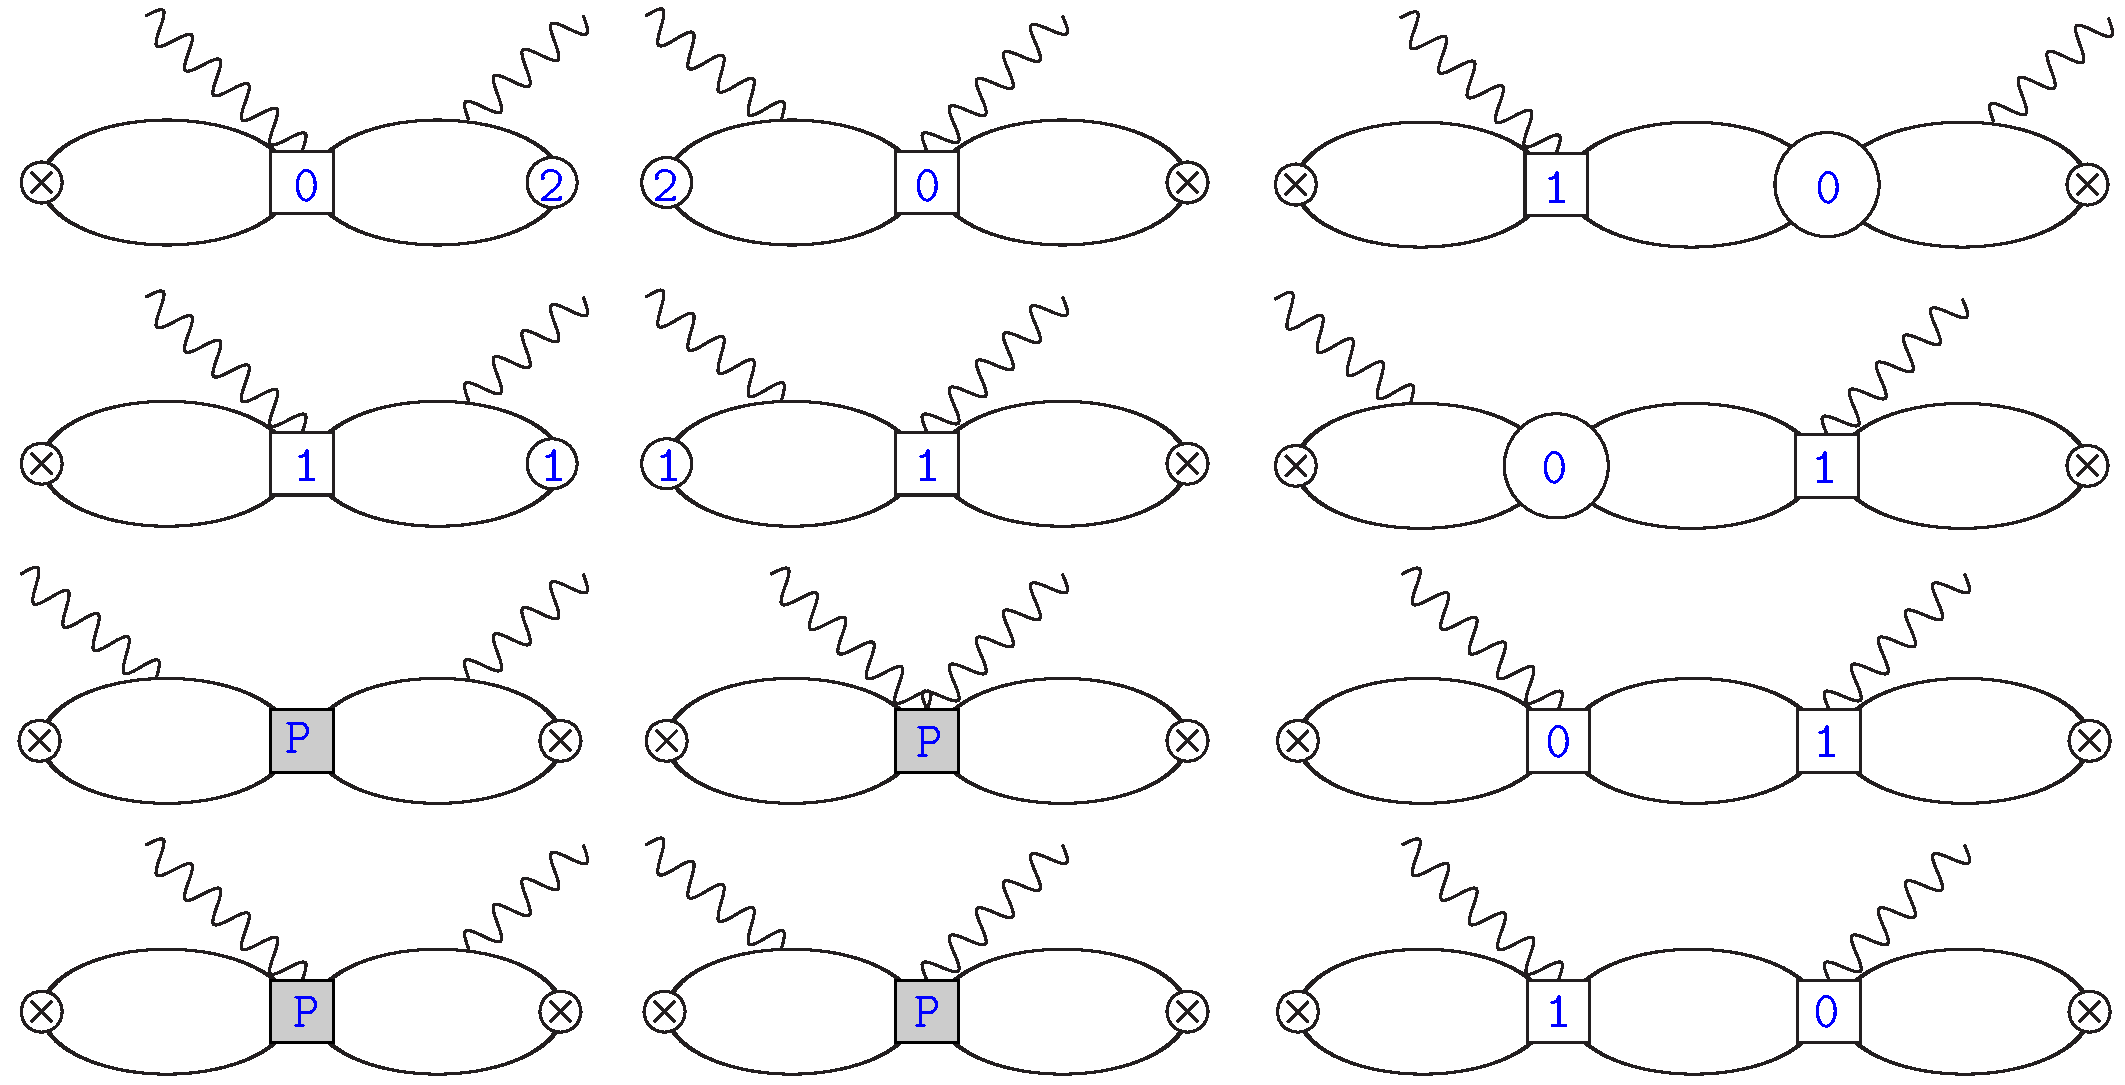
\includegraphics[width=\textwidth]{figs/VVCS_NNNLO_Pt2_v1.pdf}
    \caption{Diagrams that contribute to $\mathcal{M}_L$ at N3LO, i.e., $O(P^0)$, due to N3LO terms in the $NN$ interaction. In addition to diagrams that actually contribute to $f_L$, we also show those that are necessary in order to keep the electromagnetic gauge invariance. Grey squares marked by "P" show insertions of the $P$-wave $NN$ interactions. The rest of the notation is as in Fig.~\ref{fig:NNLO}. Crossed graphs are not shown.}
    \label{fig:NNNLO}
\end{figure}
The diagrams in Fig.~\ref{fig:NNNLO} produce a $\mu$-dependent result, and all four electric contact terms are needed in order to render the total result RG invariant.
\begin{figure}[htb]
    \centering
    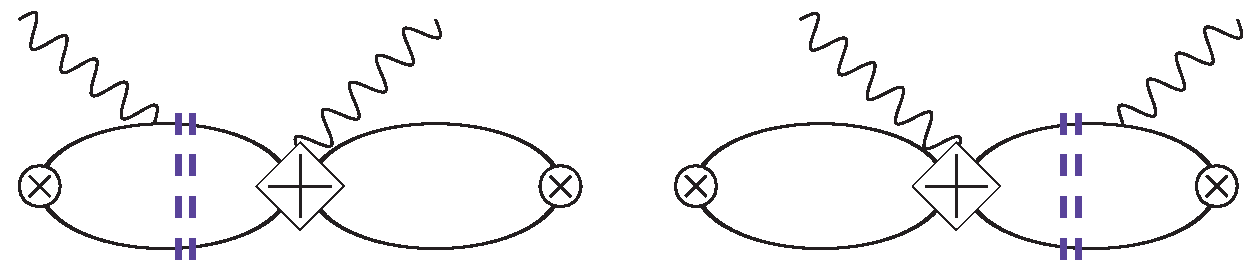
\includegraphics[width=0.6\textwidth]{figs/VVCS_NNNLO_CT_v1.pdf}
    \caption{Contributions to $\mathcal{M}_L$ at NNNLO due to the electric contact terms (shown as crossed diamonds). The rest of the notation is as in Fig.~\ref{fig:NNLO}. Crossed graphs are not shown.}
    \label{fig:NNNLO_CT}
\end{figure}
The couplings of these contact terms contribute to $\mathcal{M}_L^{(0)}$ in the following combinations with the $NN$ couplings that have to be $\mu$-independent:
\begin{align}
\mu\frac{\mathrm{d}\hphantom{\mu}}{\mathrm{d}\mu} \left[
\frac{L_1^{E1_V}-\frac{1}{2}M\, \tilde{C}_4^{(-2)}}{C_0^{(-1)}}
\right] & = 0\,,\qquad 
\mu\frac{\mathrm{d}\hphantom{\mu}}{\mathrm{d}\mu} \left[
\frac{L_3^{E1_V}-\frac{1}{2}M\, C_6^{(-4)}}{C_0^{(-1)}}
\right] = 0\,,\\
\mu\frac{\mathrm{d}\hphantom{\mu}}{\mathrm{d}\mu} \left[
\frac{L_1^{C0_S}+\frac{1}{4}M\,\tilde{C}_4^{(-2)}}{\left[C_0^{(-1)}\right]^2}
\right] & = 0\,,\qquad
\mu\frac{\mathrm{d}\hphantom{\mu}}{\mathrm{d}\mu} \left[
\frac{L_3^{C0_S}+\frac{1}{4}M\, C_6^{(-4)}}{\left[C_0^{(-1)}\right]^2}
\right] = 0\,.
\end{align}
\textcolor{blue}{This needs further clarification because~\cite{Rupak:1999rk} seems to have a factor of $2$ in the second equation.}
The first two equations have been previously obtained in Refs.~\cite{Chen:1999bg,Rupak:1999rk};
our version, however, contains an additional factor $1/2$ in front of the nucleon mass in both equations, at variance with these references. We suspect this to be due to an underestimated contribution of the contact terms to the $np\to d\gamma$ amplitude, which we also cross-checked reproducing the relevant pieces. The second pair of equations is new, to the best of our knowledge.

Considering the $\mu$ running of the quantities entering these RG equations at high momentum scales $\mu\simeq m_\pi$, one can conclude that
\begin{align}
L_1^{E1_V}-\frac{1}{2}M\, \tilde{C}_4^{(-2)}&=O(P^{-1}) \,,\qquad 
L_3^{E1_V}-\frac{1}{2}M\, C_6^{(-4)} = O(P^{-1})\,,\\
L_1^{C0_S}+\frac{1}{4}M\,\tilde{C}_4^{(-2)}&=O(P^{-2}) \,,\qquad
L_3^{C0_S}+\frac{1}{4}M\, C_6^{(-4)} = O(P^{-2})\,.
\end{align}
The first two combinations, being $O(P^{-1})$ instead of the naively expected $O(P^{-2})$ and $O(P^{-4})$, are thus demoted to at least N4LO and N6LO, respectively. The same happens with the fourth combination, which is $O(P^{-2})$ instead of $O(P^{-4})$ and is demoted to N5LO. The only combination that gives a contribution at N3LO is the one that involves $L_1^{C0_S}$. Below, we will find its value from a fit to the deuteron charge form factor.

Note that the cancellations between the contributions of the contact terms and those of the $NN$ couplings are in fact more intricate than given by these RG equations. The $NN$ coupling constants --- all apart from $\tilde{C}_4^{(-2)}$ --- conspire to remove the poles from the NNNLO correction to the $NN$ $T$ matrix. The instances of $C_6^{(-4)}$ appearing in the RG equations are in fact combinations of all the $NN$ constants appearing at this order, so a statement that $L_3^{E1_V}$ and $L_3^{C0_S}$ cancel the contribution of $C_6^{(-4)}$ might be somewhat misleading.

As before, we write
\begin{align}
    L_1^{C0_S} =-\frac{1}{4}M\, \tilde{C}_4^{(-2)} +  \frac{\pi(Z-1)^3}{\gamma^3(\mu-\gamma)^2}\,l_1^{C0_S}\,,
\end{align}
getting the following result for the total NNNLO contribution of the diagrams in Figs.~\ref{fig:NNNLO} and~\ref{fig:NNNLO_CT}:
\begin{align}
    \mathcal{M}_L^{(0)} &=
    \frac{e^2M^3}{\pi}\frac{Q^2}{\bv{q}^2}\frac{(Z-1)^3}{\gamma^3}
    \Bigg[
    \frac{3 \gamma -\lambda_d}{2(\gamma -\lambda_d)}
    +\frac{2l_1^{C0_S}\, \bv{q}^2+(\gamma -\lambda_d)^2}{8 |\bv{q}|(\gamma-\lambda_d)}\phi(\nu,\bv{q}^2)
    -\frac{\gamma^2-\lambda_d^2 }{8 \gamma ^3 \bv{q}^2}\phi^2(\nu,\bv{q}^2)
    \Bigg]\nonumber \\
    &-\frac{e^2M^3}{\pi}\frac{Q^2}{\bv{q}^2}\frac{w_2 \left[|\bv{q}|-2 (\gamma +\lambda_d)\phi(\nu,\bv{q}^2)   \right]^2}{4 \bv{q}^2} \nonumber\\
    &+\frac{e^2M^3}{\pi}\frac{Q^2}{\bv{q}^2}
   \frac{M\,C_{{}^{3\!}P_J}\left[2 q (\gamma-\lambda_d)-\left(4 \gamma ^2-4 \lambda_d^2+\bv{q}^2\right) \phi(\nu,\bv{q}^2)\right]^2}{192 \pi  \bv{q}^4}
    +(\nu\to-\nu)\,.
\end{align}
The nucleon charge radii corrections at this order are
\begin{figure}[htb]
    \centering
    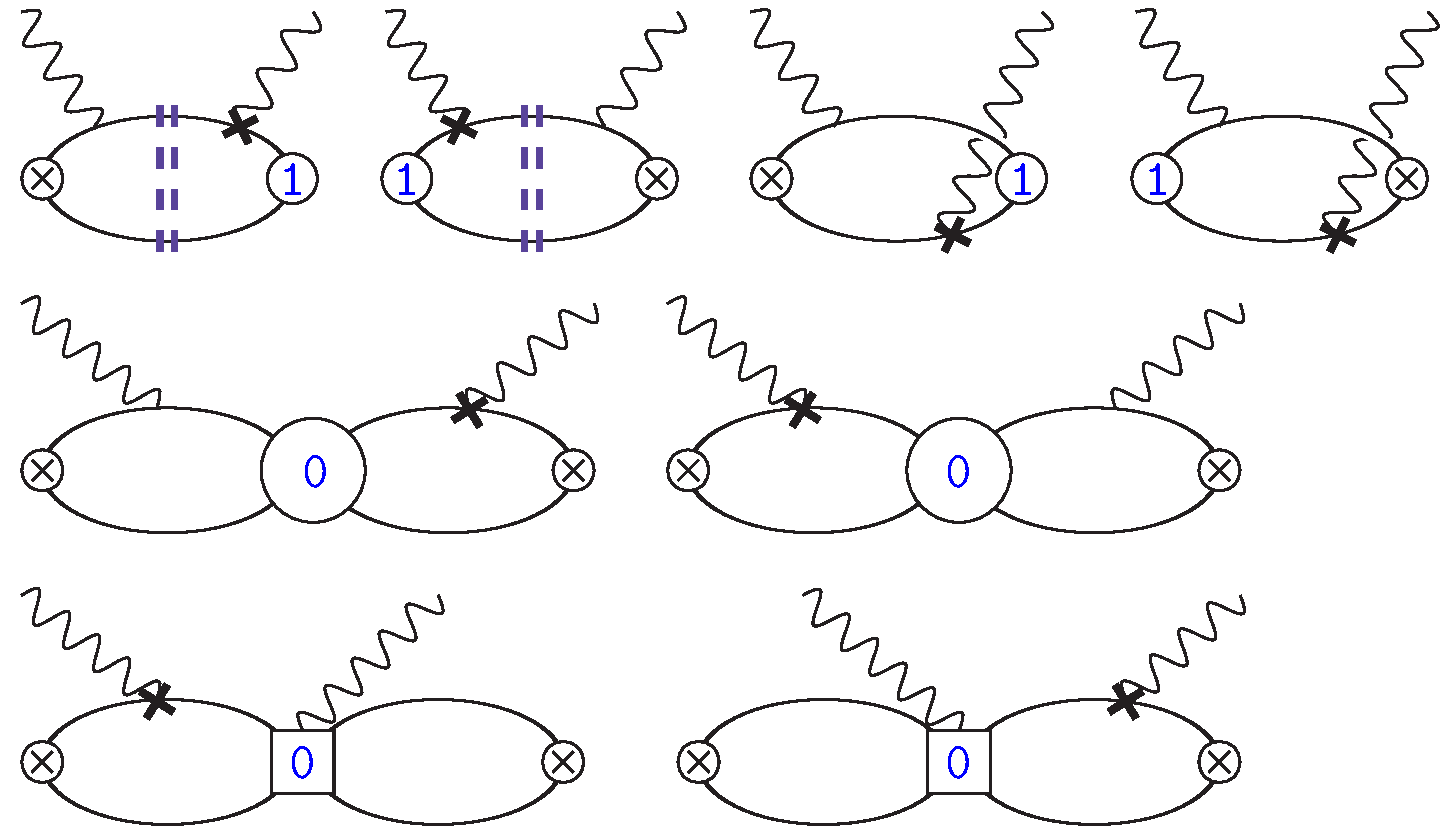
\includegraphics[width=0.7\textwidth]{figs/VVCS_NNNLO_RENucl.pdf}
    \caption{Correction to $i\mathcal{M}_L$ due to the photon coupling proportional to $\hat{r}^2$, contributing at $O(P^0)$. The rest of the notation is as in Figs.~\ref{fig:NNLO} and~\ref{fig:NNLO_RE}. Crossed graphs are not shown.}
    \label{fig:NNNLO_RE}
\end{figure}
\begin{align}
\delta\mathcal{M}_{L}^{(0)} & = -\frac{e^2 M^3}{3\pi}\frac{Q^2}{\bv{q}^2}
\frac{r_0^2 (Z-1)}{\gamma}\frac{\phi(\nu,\bv{q}^2)\left[|\bv{q}|-(\gamma +\lambda_d)\phi(\nu,\bv{q}^2)\right]}{\gamma-\lambda_d}+(\nu\to-\nu)\,.
\end{align}

\section{Deuteron charge form factor at N3LO: fitting \boldmath $l_1^{C0_S}$}
In order to extract the deuteron form factors, we use the residues of the pole parts of the VVCS amplitude. Using the elastic structure functions~\cite{Carlson:2013xea}, one can obtain:
\begin{align}
    \res f_L(\nu,Q^2)\big|_{\nu=Q^2/(2M_d)} & = - e^2\left(1+\tau_d\right)
    \left[G_C^2(Q^2)+\frac{8}{9}\tau_d\,G_Q^2(Q^2)\right]\,,\\
    \res f_T(\nu,Q^2)\big|_{\nu=Q^2/(2M_d)} & = -\frac{2}{3}e^2 \tau_d\left(1+\tau_d\right) G_M^2(Q^2)\,,
\end{align}
where $G_C(Q^2)$, $G_M(Q^2)$, and $G_Q(Q^2)$ are the deuteron charge, magnetic, and quadrupole form factors, and $\tau_d=Q^2/(4M_d^2)$. At the order we are working, $1+\tau_d=1$, and $G_Q(Q^2)=0$. The shift of the elastic poles, which appear at $\nu=\pm\bv{q}^2/(4M)$, is also a relativistic correction that can be neglected at this order, allowing one to replace $\bv{q}^2\to Q^2$ in the amplitudes when taking the residues. This results in
\begin{align}
    \res f_L(\nu,Q^2)\big|_{\nu=Q^2/(4M)} & = - e^2\, G_C^2(Q^2)\,,\\
    \res f_T(\nu,Q^2)\big|_{\nu=Q^2/(4M)} & = -\frac{e^2}{24}\frac{Q^2}{M^2}\, G_M^2(Q^2)\,.
\end{align}
Evaluating the residues and expanding the square root of $G_C^2(Q^2)$ and $G_M^2(Q^2)$ order by order gives
\begin{align}
    G_C(Q^2) & =\frac{4 \gamma}{Q} \arctan\frac{Q}{4 \gamma } \nonumber\\
    & -(Z-1) \left(1-\frac{4 \gamma}{Q}\arctan\frac{Q}{4 \gamma}\right)\nonumber\\
    &-\frac{4}{3}r_0^2\, \gamma\,  Q  \arctan\frac{Q}{4 \gamma } \nonumber\\
    &+\frac{1}{3}(Z-1)\, r_0^2\,  Q^2\left(1-\frac{4 \gamma}{Q}\arctan\frac{Q}{4 \gamma }\right)-\frac{(Z-1)^3\,l_1^{C0_S}}{2 \gamma ^2} Q^2 \,, \\
   \frac{e}{2M_d} G_M(Q^2) = \frac{e}{2M}\Bigg[& (\mu_n+\mu_p)\frac{4\gamma}{Q}\arctan\frac{Q}{4\gamma}\nonumber\\
    &-(\mu_n+\mu_p)(Z-1)\left(1-\frac{4\gamma}{Q}\arctan\frac{Q}{4\gamma}\right)
    +\frac{2}{\pi}M L_2^{M1_S}\gamma(\mu-\gamma)^2
    \Bigg]\,,
\end{align}
at NNNLO for $G_C(Q^2)$ and at NLO for $G_M(Q^2)$. The expresion for $G_M(Q^2)$ coincides with that obtained in Ref.~\cite{Chen:1999tn} (where the $\gamma \rho_d$ factor in the NLO term has to be replaced by $(Z-1)$ to account for the difference between the $Z$ and $\rho$ expansion schemes). The charge form factor has been previously calculated up to NNLO in the $Z$ expansion in Ref.~\cite{Phillips:1999hh}, whose results we also reproduce here.

The order-by-order expression for the deuteron charge radius reads
\begin{align}
    r_d^2 = -6\frac{\mathrm{d}G_C(Q^2)}{\mathrm{d}Q^2}\bigg|_{Q^2=0} & =
    \frac{1}{8 \gamma ^2}
    +\frac{Z-1}{8 \gamma ^2}
    +2r_0^2
    +\frac{3(Z-1)^3}{\gamma ^2}\,l_1^{C0_S}\nonumber \\
    & = \left[2.3325+1.6038+0.6241+18.1969\, l_1^{C0_S} \right]\text{ fm}^2\,.
\end{align}
One has to note that the NNLO result $r_d^2=4.5604\text{ fm}^2$ is already very close to the experimentally measured values, for instance, muonic deuterium spectroscopy gives $r_d^2=4.5183(33)\text{ fm}^2$~\cite{Pohl669}. This results in a tiny value of the $l_1^{C0_S}$ coupling,
\begin{align}
    l_1^{C0_S}=-2.31(18)\times 10^{-3}\,,
\end{align}
similar to what happens with $l_2^{M1_S}$. The uncertainty is calculated using the quoted experimental error of the muonic deuterium result; considering other empirical values of $r_d^2$ on the market will significantly increase the uncertainty, albeit leaving $l_1^{C0_S}$ at a level of at most $10^{-2}$.

Fig.~\ref{fig:GC} shows the deuteron charge form factor at the different orders, compared with the parametrisation of Ref.~\cite{Abbott:2000ak}. Note that the form factor of Abbott et al.\ has a smaller value of $r_d^2=4.3608\text{ fm}^2$. One can see that the shape of the deuteron form factor is very well reproduced even at values of $Q$ beyond the formal range of validity of \piEFT/. 
\begin{figure}[htb]
    \centering
    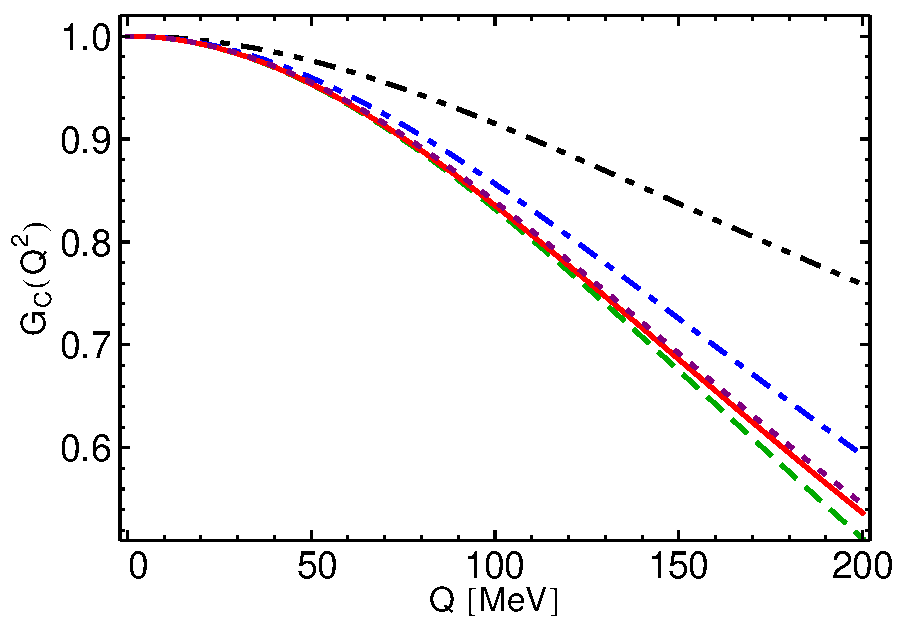
\includegraphics[width=0.6\columnwidth]{figs/GC.pdf}
    \caption{Deuteron charge form factor at LO (dash-dot-dotted black), NLO (dash-dotted blue), NNLO (dashed green), and NNNLO (solid red). The parametrisation of Ref.~\cite{Abbott:2000ak} is shown by the purple dotted curve.}
    \label{fig:GC}
\end{figure}

\section{Deuteron generalised polarisabilities}
Having determined the value of $l_1^{C0_S}$ (which appears to be unnaturally small), we turn to the (generalised) polarisabilities of the deuteron. We start from the electric and magnetic dipole polarisabilities, the results for which are
\begin{align}
    \alpha_{E1} & = \frac{\alpha M}{32\gamma^4}\left[1+(Z-1)+0+\frac{M\gamma^3}{6\pi}C_{{}^{3\!}P_J}\right] \nonumber \\
    & = [0.3775+0.2596+0-0.0018]\text{ fm}^3 = 0.6354\text{ fm}^3\,,\\
    \beta_{M1} & = \frac{\alpha}{32M\gamma^2}
    \bigg[-1+\frac{16}{3}\mu_1^2-\frac{32}{3}\mu_1^2\frac{\gamma}{\gamma_s-\gamma } \nonumber \\
&\hphantom{=\frac{\alpha}{32M\gamma^2}\bigg[\,\,}
+\frac{Z-1}{3} \left(16\mu_1^2-3\right)
-\frac{32(Z-1)}{3}\mu_1(\mu_1+l_1^{M1_V}) \frac{\gamma}{\gamma_s-\gamma}
+\frac{16}{3}\mu_1^2 r_s \frac{\gamma^3}{(\gamma_s-\gamma)^2}
   \bigg]\nonumber\\
& = [0.0703-0.0001]\text{ fm}^3 = 0.0702\text{ fm}^3\,.
\end{align}
The expression for $\alpha_{E1}$ reproduces the NNNLO result obtained in Ref.~\cite{Phillips:1999hh} using the $np\to\gamma d$ cross section calculated in Ref.~\cite{Rupak:1999rk}, however, our $P$-wave contribution is a factor of $2$ smaller (which we also cross-checked, reproducing the relevant terms in the $np\to d\gamma$ cross section). The numerical value is in agreement with, e.g., the recent $\chi$EFT-based evaluation of Ref.~\cite{Acharya:2020bxf} that obtained $\alpha_{E1}=0.626(18)\text{ fm}^3$. 

The LO expression for $\beta_{M1}$ reproduces the result of Ref.\cite{Ji:2003ia}, and the NLO result is new. The numerical value is also in a very good agreement with the result of Ref.~\cite{Acharya:2020bxf}, $\beta_{M1}=0.0715(15)\text{ fm}^3$; this agreement looks remarkable, given that it is a relatively low-order calculation. The cancellation of the NLO terms, giving essentially a zero NLO contribution to $\beta_{M1}$, appears even more surprising. Both these results could be attributed to the procedure used in Ref.~\cite{Rupak:1999rk} to fit the value of $L_1^{M1_V}$ to reproduce the $np\to d\gamma$ cross section at NLO. Indeed, if this cross section is well described in \piEFT/, one should also expect a good description of the transverse response function of the deuteron at small non-zero $Q^2$. This, by virtue of the sum rule for $\beta_{M1}$ derived in Ref.~\cite{Gorchtein:2015eoa}, should be sufficient in order to reproduce the value of $\beta_{M1}$ at NLO, explaining at the same time the vanishing NLO contribution. This explanation, however, may imply that the description of the response function has to remain satisfactory up to relatively high energies outside of the validity of \piEFT/; while this could be the case, investigating it in further detail is outside of the scope of this work.

The generalisation of $\alpha_{E1}$ and $\beta_{M1}$ to finite $Q^2$ is defined the usual way,
\begin{align}
    \alpha_{E1}(Q^2) = \frac{f_L(0,Q^2)}{4\pi Q^2}\,,\qquad 
    \beta_{M1}(Q^2)  = \frac{\bar{f}_T(0,Q^2)}{4\pi Q^2}\,,
\end{align}
where $\bar{f}_T$ stands for the non-pole part of $f_T$ with the Thomson term subtracted as well. The resulting curves are showin in Fig.~\ref{fig:alpha_beta}.
\begin{figure}[htb]
    \centering
    \begin{tabular}{cc}
    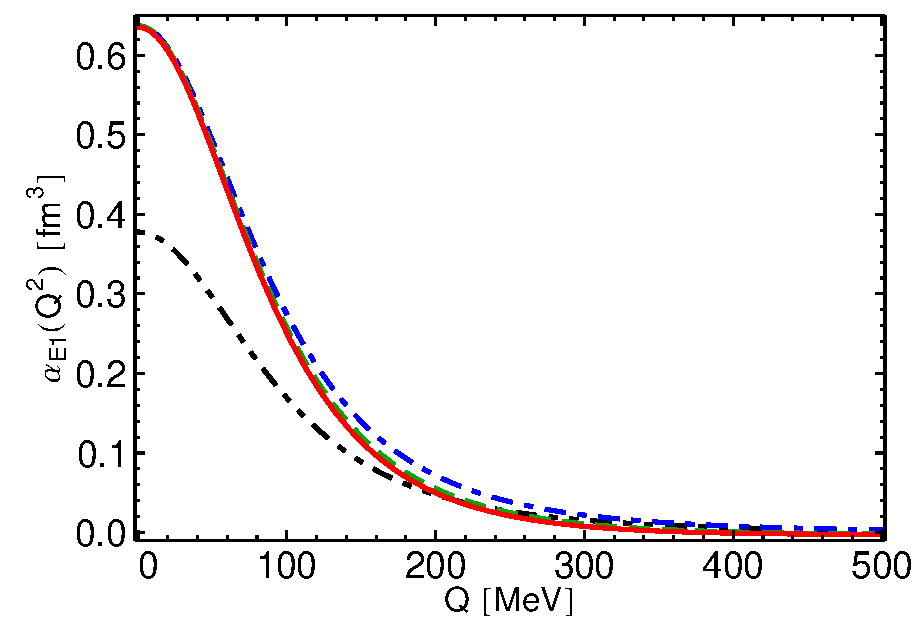
\includegraphics[width=0.5\textwidth]{figs/alphaE.pdf} &
    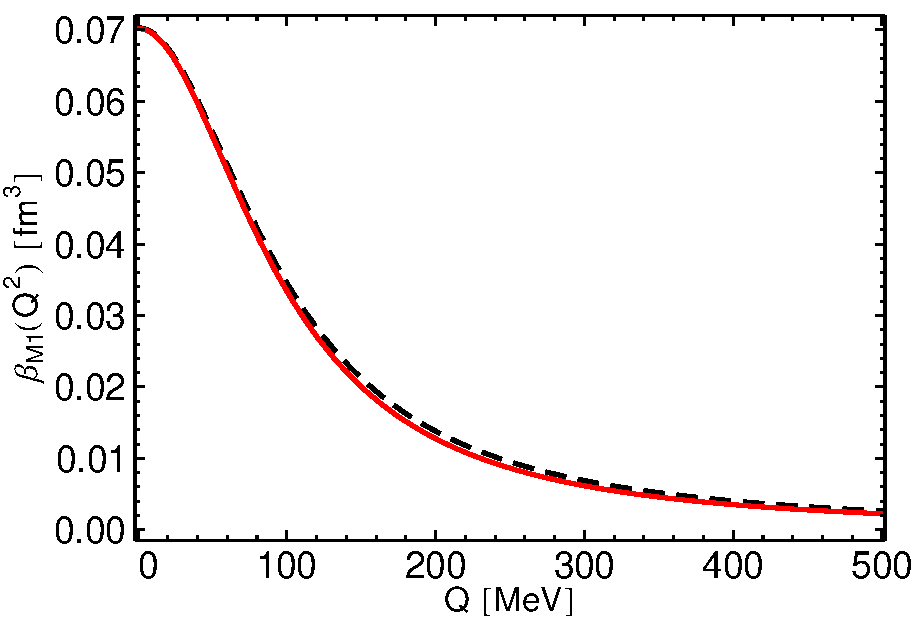
\includegraphics[width=0.5\textwidth]{figs/betaM.pdf}
    \end{tabular}
    \caption{Generalised deuteron polarisabilities $\alpha_{E1}(Q^2)$ (left panel) and $\beta_{M1}(Q^2)$ (right panel). The LO, NLO, NNLO, and NNNLO results for $\alpha_{E1}(Q^2)$ in the left panel are coded as in Fig.~\ref{fig:GC}. In the right panel, the LO and NLO results for $\beta_{M1}(Q^2)$ are shown, respectively, by the black dashed and the red solid curve.}
    \label{fig:alpha_beta}
\end{figure}
\textcolor{blue}{What else can we write here about those curves?} \textcolor{magenta}{Something about convergence (maybe with percentages): Note that for $\beta_{M1}$ a good convergence is already achieved at its LO (which, strictly speaking corresponds to a NNLO calculation, since the contributions to $\beta_{M1}$ start two orders higher than $\alpha_{E1}$). For $\alpha_{E1}$, a large correction still arises at NLO and one has a non-negligible contribution even at NNLO. Also, do we have any other works to compare to?}

It is also interesting to consider two further generalised polarisabilities, namely, the longitudinal polarisability $\alpha_L(Q^2)$ and the generalised Baldin sum rule $[\alpha_{E1}+\beta_{M1}](Q^2)$, defined as
\begin{align}
\alpha_L(Q^2) = \frac{1}{4\pi Q^2}\frac{\mathrm{d}f_L(\nu,Q^2)}{\mathrm{d}\nu^2}\bigg|_{\nu=0} \,, \qquad
[\alpha_{E1}+\beta_{M1}](Q^2)=\frac{1}{4\pi}\frac{\mathrm{d}f_T(\nu,Q^2)}{\mathrm{d}\nu^2}\bigg|_{\nu=0}\,.
\end{align}
The $Q^2=0$ value of $\alpha_L$ is given by
\begin{align}
    \alpha_L & = \frac{7\alpha M^3}{768\gamma^8}\left[1+(Z-1)+0+\frac{11M\gamma^3}{126\pi}C_{{}^{3\!}P_J}\right]\nonumber\\
    & = \left[0.867+0.596+0-0.002\right]\times 10^3\text{ fm}^5=1.461\times 10^3\text{ fm}^5\,.
\end{align}
For the sake of simplicity, this result is obtained by substituting $|\bv{q}|\to Q$ in the expressions for $f_L$ obtained above and thus neglects relativistic corrections of a relative size of roughly $0.2\%$. One can see that higher deuteron moments, such as $\alpha_L$, are numerically enhanced, unlike what happens in the case of the nucleon, see, e.g, Ref.~\cite{Alarcon:2020wjg}.

The $Q^2=0$ value of the Baldin sum rule coincides with the NLO result for $\alpha_{E1}+\beta_{M1}$ given above. Strictly speaking, this includes corrections beyond NLO, because $\beta_{M1}$ starts two orders higher than $\alpha_{E1}$, however, the explicit gauge invariance allows one to recover $\beta_{M1}$ by substituting $|\bv{q}|=\sqrt{Q^2+\nu^2}$ instead of neglecting $\nu$. Using $\bv{q}=Q$, on the other hand, changes the value of $[\alpha_{E1}+\beta_{M1}](Q^2)$ by about $10\%$ at $Q^2=0$ (by dropping the static value of $\beta_{M1}$). The difference quickly decreases with growing $Q$ and becomes negligible already at $Q\simeq 20$~MeV.
\begin{figure}[htb]
    \centering
    \begin{tabular}{cc}
    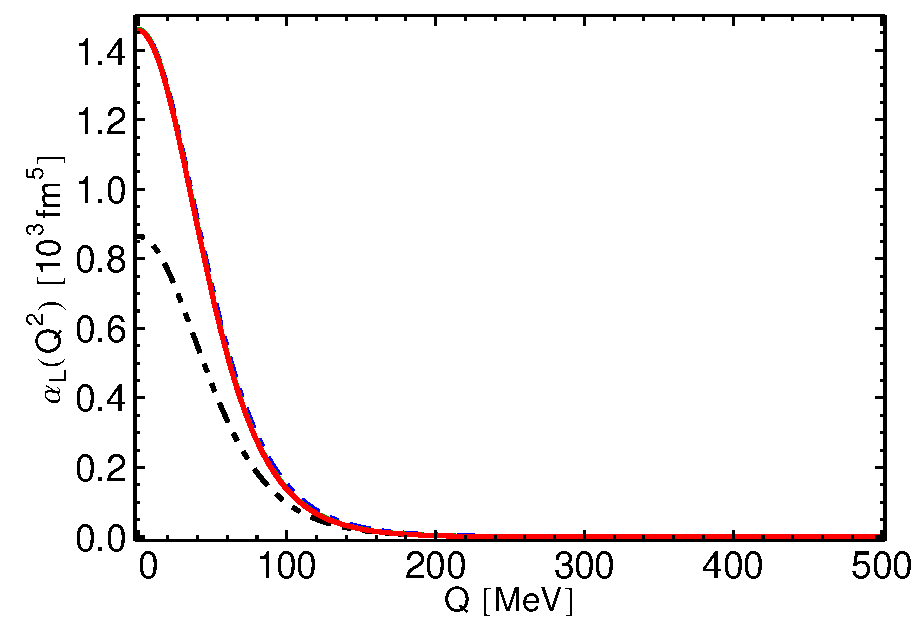
\includegraphics[width=0.5\textwidth]{figs/alphaL.pdf} &
    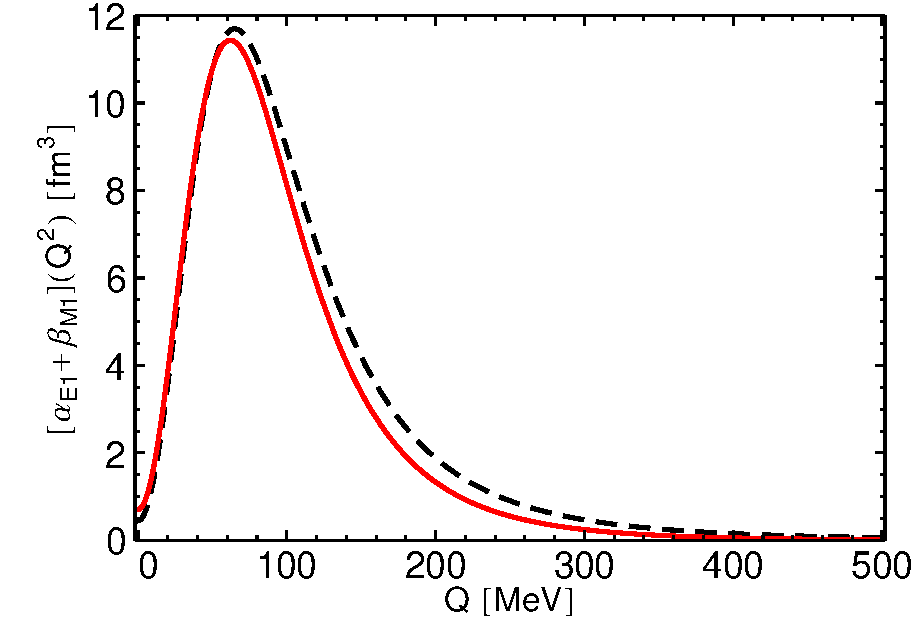
\includegraphics[width=0.5\textwidth]{figs/BSR.pdf}
    \end{tabular}
    \caption{Deuteron longitudinal polarisability $\alpha_{L}(Q^2)$ (left panel) and the generalised Baldin sum rule $[\alpha_{E1}+\beta_{M1}](Q^2)$ (right panel). The curves are coded as in the left and right panel of Fig.~\ref{fig:alpha_beta}, respectively.}
    \label{fig:alphaL_BSR}
\end{figure}

The curves for $\alpha_L(Q^2)$ and $[\alpha_{E1}+\beta_{M1}](Q^2)$ are shown in Fig.~\ref{fig:alphaL_BSR}. One can see that the longitudinal polarisability shares the general features of the previously considered $\alpha_{E1}(Q^2)$ and $\beta_{M1}(Q^2)$, with a somewhat quicker falloff with growing $Q$. The generalised Baldin sum rule, on the other hand, demonstrates a sharp increase peaking around $Q=60$~MeV; this enhancement is due to the magnetic interaction in the singlet channel and is analogous to what has been seen, e.g., for the generalised spin-forward deuteron polarisability $\gamma_0(Q^2)$~\cite{Lensky:2018vdq}.

\section{TPE correction in muonic deuterium}
\begin{figure}[htb]
    \centering
    \begin{tabular}{cc}
    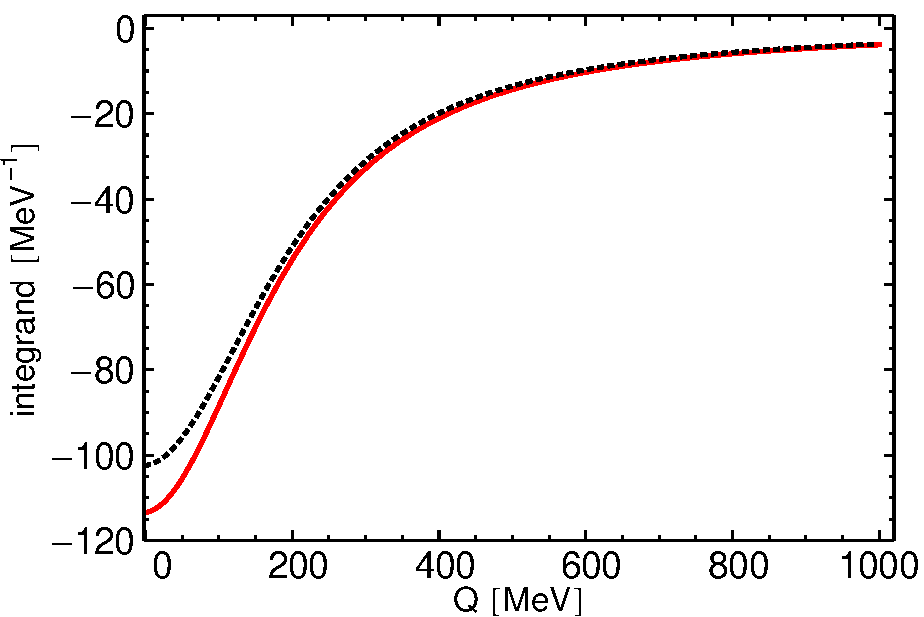
\includegraphics[width=0.5\textwidth]{figs/elastic.pdf}
    &
    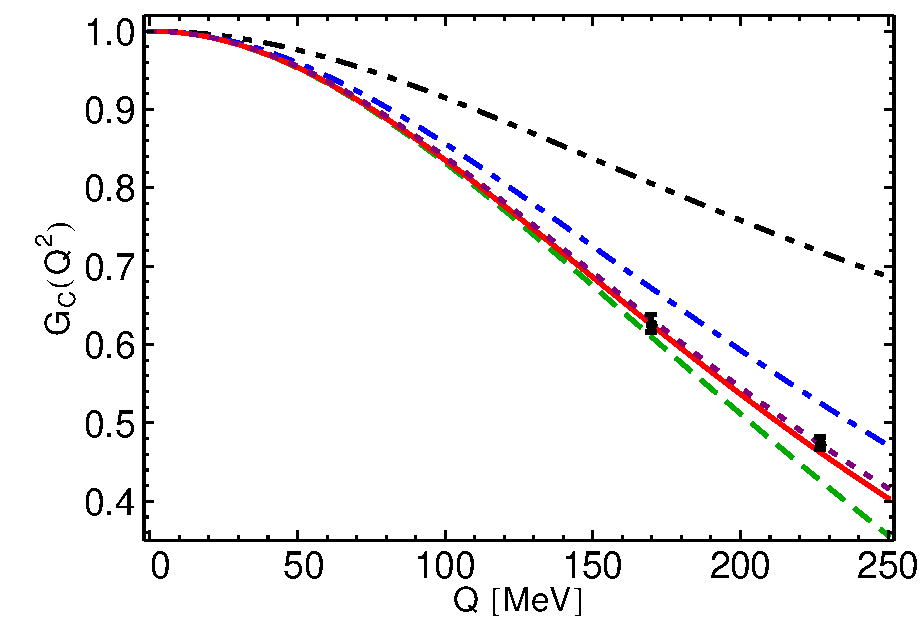
\includegraphics[width=0.5\textwidth]{figs/GCdata.pdf}
    \end{tabular}
    \caption{Left panel: Integrand of Eq.~\eqref{eq:contrib_elastic} as function of $Q$. Black dotted: parametrisation of Ref.~\cite{Abbott:2000ak}; red solid: results of the \piEFT/ calculation. Right panel: $G_C(Q^2)$ compared with data from Ref.~\cite{Abbott:2000ak} (black dots). The curves are denoted as in Fig.~\ref{fig:GC}.}
    \label{fig:elastic_integrand}
\end{figure}
%\subsection{Results}
The elastic contribution is given by~\cite{Carlson:2013xea}
\begin{align}
\Delta E_{n\ell}^\mathrm{elastic} & = \frac{m \alpha^2}{M_d(M_d^2-m^2)}[\phi_{n\ell}(0)]^2
\int\limits_0^\infty\frac{\mathrm{d}Q^2}{Q^2} 
 \times\left\{
\frac{2}{3}G_M^2(Q^2)
(1+\tau_d)\hat{\gamma}_1(\tau_d,\tau_l)
%\left(\frac{\gamma_1(\tau_d)}{\sqrt\tau_d}-\frac{\gamma_1(\tau_l)}{\sqrt\tau_l}\right)
- \right. \nonumber\\
& \qquad \left. %\left(\frac{\gamma_2(\tau_d)}{\sqrt\tau_d}-\frac{\gamma_2(\tau_l)}{\sqrt\tau_l}\right)
\left[\frac{G_C^2(Q^2)-1}{\tau_d}+\frac{2}{3}G_M^2(Q^2)+\frac{8}{9}\tau_d G_Q^2(Q^2)\right]
\hat{\gamma}_2(\tau_d,\tau_l)
\right. +16M_d^2\frac{M_d-m}{Q}G_C'(0)
\bigg\}\,,\label{eq:contrib_elastic}
\end{align}
where the weighting functions are defined by
\begin{align}
\hat{\gamma}_{1,2}(x,y) & = \frac{\gamma_{1,2}(x)}{\sqrt{x}}-\frac{\gamma_{1,2}(y)}{\sqrt{y}}\,,\\
\gamma_1(x) & = (1-2x)\sqrt{1+x}+2x^{3/2}\,,\\
\gamma_2(x) & = (1+x)^{3/2}-x^{3/2} -\frac{3}{2}\sqrt{x}\,,
\end{align}
and $\tau_l=Q^2/(4m^2)$. The contributions of point-like charge and charge radius of the deuteron
are removed from the elastic part to avoid double-counting. The value obtained in Ref.~\cite{Carlson:2013xea} is
\begin{align}
    \Delta E_{2S}^\mathrm{elastic} & = -0.417(2) \text{ meV}\,,
\end{align}
using the deuteron form factors from Ref.~\cite{Abbott:2000ak}; the uncertainty is estimated using the different form factor parametrisations derived in~\cite{Abbott:2000ak}. It is instructive to repeat this calculation, separating the different form factors in Eq.~\eqref{eq:contrib_elastic}; we obtain
\begin{align}
    \Delta E_{2S}^\mathrm{elastic} & = -0.4152 + 0.0001-0.0007 = -0.4158\text{ meV}\,,
\end{align}
where the numbers stand for the contributions of $G_C(Q^2)$, $G_M(Q^2)$, and $G_Q(Q^2)$, in order. One can see that both the magnetic and quadrupole form factors give a negligible contribution to the elastic part of the TPE correction. 

The \piEFT/ calculation of $G_C(Q^2)$ and $G_M(Q^2)$ allows one to calculate the elastic contribution as well: with the NNNLO result for $G_C^2(Q^2)$ and the NLO result for $G_M(Q^2)$, the integral in Eq.~\eqref{eq:contrib_elastic} converges at large $Q$. This results in
\begin{align}
    \Delta E_{2S}^\mathrm{elastic}=-0.2046-0.1580-0.0626-0.0208 = -0.4460 \text{ meV}\,,
\end{align}
where the numbers stand for the order-by-order contributions. This is somewhat larger in magnitude than the expression obtained with the empirical form factors of Ref.~\cite{Abbott:2000ak}.

Friar and cubic radius:

\begin{align}
    r_\mathrm{F} &= 3.2919\text{ fm (Abbott)}\,,\qquad r_\mathrm{F} = 3.3753\text{ fm (\piEFT/)}\\
    r_3          &= 2.4012\text{ fm (Abbott)}\,,\qquad r_3          = 2.4677\text{ fm (\piEFT/)}\,.
\end{align}
The \piEFT/ quantities here have the following analytic expressions:
\begin{align}
    r_F^3 & = \frac{3}{80\gamma^3}\left\{
    Z \left[5 - 2 Z (1-2\ln 2)\right]-\frac{320}{9} r_0^2\gamma ^2 \left[Z(1-4\ln 2)-2+2\ln 2\right]
    +
    80 (Z-1)^3 l_1^{C0_S}\right\}\,, \\
    r_3^3 & = \frac{Z}{\gamma^3}\left[\frac{3}{32}+r_0^2\gamma^2\right]\,.
\end{align}
\textcolor{blue}{Perhaps the notation for the nucleon radius $r_0^2$ should be changed in order to avoid confusion.}

The calculation of the inelastic part of TPE correction with the known $f_L(\nu,Q^2)$ is straightforward. The only technical complication is that the longitudinal term in the integral of Eq.~\ref{eq:LS_from_LT} goes as $f_L(0,Q^2)/Q^3\propto 1/Q$ as $Q\to 0$ when one sets $x=0$. This singularity, however, is spurious, and can be avoided by subtracting from $f_L(\nu,Q^2)$ its static part:
\begin{align}
    f_L(\nu,Q^2) & = f_L(0,Q^2) + \left[f_L(\nu,Q^2)-f_L(0,Q^2)\right]\,.
\end{align}
The integration over $x$ in the integral of $f_L(0,Q^2)$ can be done analytically, resulting in a $f_L(0,Q^2)/Q^2\propto Q^0$ behaviour as $Q\to 0$. At the same time, the difference in the square brackets is $O(x^2)$ at small $x$ and therefore cancels the singularity in the weighting function.

The results for the inelastic part of the TPE correction in muonic deuterium are shown order-by-order in Table~\ref{tab:TPE_results}.
\begin{table}[hbt]
\begin{tabular}{c||c c c c|| c}
                         & LO       & NLO       & NNLO      &\ NNNLO   & Total\\
\hline
\hline
$\Delta E_{2S}^\mathrm{inel}$ [meV]    &\parbox{0.1\textwidth}{$-0.944$} & \parbox{0.1\textwidth}{$-0.634$}  & \parbox{0.1\textwidth}{$\hpm 0.049$}  & \parbox{0.1\textwidth}{$\hpm 0.025$} & \parbox{0.11\textwidth}{$-1.505(18)$}    
\end{tabular}
\caption{Results for the inelastic TPE contribution.}
\label{tab:TPE_results}
\end{table}
To analyse the contributions in detail, we split them as shown in Table~\ref{tab:TPE_contributions}, keeping track of different terms appearing both due to the $(Z-1)$ factors coming from the NLO piece of $\Sigma^\prime(E_d)$ and due to new sources at each order in $\mathcal{M}_L$.
\begin{table}[htb]
    \centering
    \begin{tabular}{cc}
         \hline
         LO & NLO\\
         \hline
         \parbox{0.4\textwidth}{
         \begin{align}
             \Delta E^{(-3)}      & =   - 0.9442\nonumber\\
              & \nonumber
         \end{align}
         }
         & \parbox{0.4\textwidth}{
         \begin{align}
             (Z-1)\Delta E^{(-3)} & =   - 0.6492 \nonumber \\
             \Delta E^{(-2)}      & =\hpm 0.0153 \nonumber
         \end{align}
         }\\
         \hline\hline
          NNLO & NNNLO \\
          \hline
         \parbox{0.4\textwidth}{
         \begin{align}
             (Z-1)\Delta E^{(-2)} & =\hpm 0.0105 \nonumber\\
             \Delta E^{(-1)}      & =   - 0.0006 \nonumber\\
           \Delta E^{(-1)}_{r_N^2}& =\hpm 0.0389 \nonumber\\
             & \nonumber \\
             & \nonumber \\
             & \nonumber \\
             & \nonumber 
         \end{align}
         }
         & \parbox{0.4\textwidth}{
         \begin{align}
             (Z-1)\Delta E^{(-1)} & =   - 0.0004 \nonumber\\
      (Z-1)\Delta E^{(-1)}_{r_N^2}& =\hpm 0.0267 \nonumber\\
                    \Delta E^{(0)}& =   - 0.0009 \nonumber\\
              \Delta E^{(0)}_{w_2}& =\hpm 0.0002 \nonumber\\
                \Delta E^{(0)}_{P}& =\hpm 0.0068 \nonumber\\
       \Delta E^{(0)}_{l_1^{C0_S}}& =   - 0.0015 \nonumber\\
            \Delta E^{(0)}_{r_N^2}& =   - 0.0063 \nonumber 
         \end{align}
         }
         \\
         \hline
    \end{tabular}
    \caption{$\Delta E_{2S}^\mathrm{inel}$ in detail: contributions appearing at each order in the expansion.
    Upper indices indicate the order of $\mathcal{M}_L$ that generates the corresponding contribution. Quantities without labels are the complete contributions at the respective order excluding the labelled terms listed separately. Labels indicate the specific terms within $\mathcal{M}_L$: $r_N^2$, $w_2$, $P$, and $l_1^{C0_S}$ stand, in order, for the nucleon charge radii correction, the contribution proportional to the shape parameter $w_2$, the $P$-wave contribution, and the contribution proportional to $l_1^{C0_S}$.  All numbers are in meV.
    }
    \label{tab:TPE_contributions}
\end{table}
This table demonstrates that, with the bulk of $\Delta E_{2S}$ coming from the $LO$ part of $\mathcal{M}_L$, the most important correction comes from the nucleon charge radii, with the second-biggest correction driven by the NLO term of $\mathcal{M}_L$. The remaining mechanisms all give much smaller contributions.

To estimate the uncertainty due to the omitted higher-order terms in the \piEFT/ expansion, we adapt the procedure suggested in Ref.~\cite{Epelbaum:2014sza}, based on the calculated terms in the expansion, to the Z expansion. Namely, we calculate the error estimate for the contributions without the $(Z-1)$ corrections, and then multiply it by $Z$:
\begin{align}
    \delta E_{2S}^\mathrm{inel} & = Z\max\left\{(\gamma/m_\pi)^4\Delta E^{(-3)},(\gamma/m_\pi)^3\Delta E^{(-2)},(\gamma/m_\pi)^2\sum_i\Delta E_i^{(-1)},(\gamma/m_\pi)\sum_i\Delta E_i^{(0)}\right\}\,,
\end{align}
resulting in the uncertainty estimate for the total result as given in Table~\ref{tab:TPE_results}. To test this estimate, we study a few further subleading effects that can be numerically important.

Results listed in Tables~\ref{tab:TPE_results} and~\ref{tab:TPE_contributions} are obtained with the substitution $|\bv{q}|\to Q$ in the expressions for $\mathcal{M}_L$; using $|\bv{q}|=\sqrt{Q^2+\nu^2}$ brings the total value to $-1.508$~meV, giving an estimate of the relativistic corrections at N4LO. One can also note that the smallness of this particular effect corroborates the choice of the counting scheme used in the calculation, namely, that the energy transfer is suppressed and $\nu/Q=O(P)$. This statement can be made more quantitative by observing that shrinking the $x$ integration interval in Eq.~\ref{eq:LS_from_LT} to $x\in[-1/3,1/3]$ retains $\sim 90\%$ of the LO$+$NLO contribution. Furthermore, the transverse contribution to $\Delta E_{2S}^\mathrm{inel}$, calculated at NLO for $f_T(\nu,Q^2)$, is small in accordance with the prediction of the \piEFT/ counting:
\begin{align}
\Delta E_{2S}^{\mathrm{inel},T}=-0.005\text{ meV}\,.
\end{align}
These observations indicate that the choice of the \piEFT/ counting works well for the present calculation, and the higher-order corrections should be under control.

The nucleon form factor corrections, being the most important ones, are also potentially the most problematic, since they are enhanced by a factor of $\bv{q}^2$ compared with the corresponding amplitude with point-like nucleons. The correction, entering at N4LO, that has two insertions of the nucleon charge radii operator in the LO diagrams for $\mathcal{M}_L$, would be enhanced by a factor of $\bv{q}^4$ and would lead to a divergent at large $Q$ contribution to $\Delta E_{2S}^\mathrm{inel}$.
This bad behaviour of the nucleon form factor correction can be improved by inserting the full nucleon form factors in the nucleon charge operator vertex, replacing
\begin{align}
\hat{Q}\to \frac{\hat{G}^N_E(Q^2)}{\sqrt{1+\frac{Q^2}{4M^2}}}\,,
\label{eq:nucleonFFs}
\end{align}
where $\hat{G}^N_E(Q^2)=G_E^{0}(Q^2)+G_E^1(Q^2)\,\tau_3$ with $G_E^{0,1}$ being the isoscalar and isovector nucleon form factors, $G_E^{0,1}(Q^2)=\left[G_E^p(Q^2)\pm G_E^n(Q^2)\right]/2$.
This replacement would change the LO and NLO contributions as follows, using the recent form factor parametrisation of Ref.~\cite{Borah:2020gte}:
\begin{align}
    \Delta E^{(-3)}\to\Delta E^{(-3)}_\mathrm{FF} =-0.9175~\text{meV}\,, \qquad 
    \Delta E^{(-2)}\to\Delta E^{(-2)}_\mathrm{FF} =0.0126~\text{meV}\,, \qquad 
\end{align}
which at the same time absorbs both $\Delta E^{(-1)}_{r_N^2}$ and $\Delta E^{(0)}_{r_N^2}$.
This would change the total result for $\Delta E_{2S}^\mathrm{inel}$ by $-0.0145$~meV. One can notice that this effect is quite significant, for instance, it is about a factor of four larger than what one obtains in a chiral EFT calculation replacing linear form factors by a realistic parametrisation~\cite{Acharya:2020bxf}. It is, however, within our error estimate. The replacement of the charge operator by the form factors in the higher-order contributions would give a negligible effect on the total result.

Another single-nucleon effect appearing at N4LO that is potentially sizeable is that of the nucleon polarisabilities. Its contribution to the deuteron VVCS amplitude leads, similarly to the aforementioned correction with two insertions of the charge radius operator, to a divergent contribution  to $\Delta E_{2S}$. A \piEFT/ consideration would therefore introduce four-nucleon, two-lepton contact terms at N4LO to regularise this divergence. An alternative is to calculate it separately using the empirical nucleon structure functions, as done in Refs.~\cite{Acharya:2020bxf,Carlson:2013xea}. The latter reference obtained $\Delta E_{2S}^\mathrm{hadr}=-0.028(2)$~meV for the total hadronic correction, which is larger than our uncertainty. We therefore choose to add this correction to our result, thus taking into account the most significant subleading single-nucleon corrections. We expect the remaining higher-order effects to be within our uncertainty estimate.

Finally, to obtain the total result for the TPE correction, one has to include the elastic part of the integral in Eq.~\ref{TPE_LS}, which gives $\Delta E_{2S}^\mathrm{elastic}=-0.417(2)$~meV~\cite{Carlson:2013xea}, as well as the formally subleading $O(\alpha^6\ln \alpha)$ Coulomb correction, which, however, is numerically important. For the latter, we take the value $\Delta E_{2S}^\mathrm{Coulomb}=0.262(2)$~meV from the compilation of Ref.~\cite{Krauth:2015nja}. This gives
\begin{align}
    \Delta E_{2S}^\mathrm{TPE} & = \Delta E_{2S}^\mathrm{inel}+\Delta E_{2S}^\mathrm{elastic}+\Delta E_{2S}^\mathrm{Coulomb}+\Delta E_{2S}^\mathrm{hadr}= -1.688(19)\text{ meV}\,.
\end{align}
Table~\ref{tab:results_comparison} compares our results with other recent calculations.

\begin{table}[]
    \centering
    \begin{tabular}{c||c|c|c|c|c|c}
    &  This work
    & Ref.~\cite{Acharya:2020bxf}
    & Ref.~\cite{Hernandez:2014pwa}
    & Ref.~\cite{Hernandez:2017mof}
    & Ref.~\cite{Hernandez:2019zcm}
    & Ref.~\cite{Emmons:2020aov}
    \\
    \hline\hline
    $\Delta E_{2S}^\mathrm{TPE}$ [meV]
    & $-1.688(19)$
    & $-1.695(13)$
    & $-1.690(20)$
    & $-1.715^{+22}_{-24}$
    & $-1.703$
    & $-1.757(80)$
    \end{tabular}
    \caption{Comparison of our results with the results of previous recent calculations. For comparison with Ref.~\cite{Hernandez:2019zcm}, we added $\Delta E_{2S}^\mathrm{hadr}$ to their ``$\eta$-less'' result. Analogously, for comparison with Ref.~\cite{Emmons:2020aov}, we added $\Delta E_{2S}^\mathrm{elastic}+\Delta E_{2S}^\mathrm{Coulomb}+\Delta E_{2S}^\mathrm{hadr}$ to their ``$\mathcal{Z}_d$ improved'' result.}
    \label{tab:results_comparison}
\end{table}

\section{Discussion}
\newpage
\begin{enumerate}
    \item Split Lamb shift from VVCS.
    \item Lamb shift:
    \begin{itemize}
        \item Add a calculation of the elastic contribution from \piEFT/.
        \item Introducing the nucleon form factors using the procedure discussed last week seems to be too difficult, and it also seems to make the longitudinal amplitude $\mu$-dependent at NLO. Therefore I suggest to use Eq.~\eqref{eq:nucleonFFs} to plug in the nucleon form factors in $f_L$ and remark that even though this procedure is not strictly gauge invariant, the gauge invariance breaking is of higher orders than we consider.
        \item Nucleon form factors: use another parametrisation as a check.
        \item Calculate the eVP correction (elastic and inelastic). Discuss the deuteron radius puzzle.
        \item Point out the correlation between $\Delta E^\mathrm{TPE}_{2S}$ and the deuteron charge radius via the coupling $L_1^{C0_S}$. The expression for $l_1^{C0_S}$ can be rewritten to emphasise it.
        \item Redo the calculation using the updated constants.
        \item \sout{Calculate deuteron Friar radius and $r^3$.}
    \end{itemize}
    \item VVCS
    \begin{itemize}
        \item Add more detail such as Feynman rules.
        \item Add equation for the counting power of a general graph.
        \item Need to sort out the deuteron form factors and the Born term discussion.
    \end{itemize}
\end{enumerate}


\appendix
\section{Feynman rules}

\section{LO amplitudes diagram by diagram}
Feynman graphs in Fig.~\ref{fig:LO} give the following contributions to $\mathcal{M}$, in order:
\begin{enumerate}
\item 
\begin{align}
    \mathcal{M}_L & = 0\,,\\
    \mathcal{M}_T & = -\frac{e^2 M}{\pi}\frac{1}{8\gamma}\,.
\end{align}
\item
\begin{align}
    \mathcal{M}_L & = \frac{e^2 M^3}{\pi}\frac{Q^2}{\bv{q}^2}\frac{1}{2 \gamma  \left[\bv{q}^2+4 (\gamma +\lambda_d)^2\right]}\,,\\
    \mathcal{M}_T & = \frac{e^2 M}{\pi}\left[-
    \frac{\gamma-\lambda_d}{4 \bv{q}^2}
    +\frac{(\mu_0^2+\mu_1^2) \bv{q}^2}{4 \gamma  \left[\bv{q}^2+4 (\gamma +\lambda_d)^2\right]}+\frac{4 \gamma ^2-4 \lambda_d^2+\bv{q}^2}{8 |\bv{q}|^3}\phi(\nu,\bv{q}^2)
   \right]
   \,.
\end{align}
\item
\begin{align}
    \mathcal{M}_L & = 0\,,\\
    \mathcal{M}_T & = \frac{e^2 M}{\pi}\frac{|\bv{q}| (\mu_0^2-\mu_1^2)}{12 M \nu}
    \left[
    \phi(\nu,\bv{q}^2) - \phi(-\nu,\bv{q}^2) 
   \right]\,.
\end{align}
\item
\begin{align}
    \mathcal{M}_L & = -\frac{e^2 M^3}{\pi}\frac{Q^2}{\bv{q}^2}\frac{1}{\bv{q}^2 (\gamma-\lambda_d)}\phi^2(\nu,\bv{q}^2)\,,\\
    \mathcal{M}_T & = -\frac{e^2 M}{\pi}\frac{2\mu_0^2}{3 (\gamma-\lambda_d)}\phi^2(\nu,\bv{q}^2)\,.
\end{align}
\item
\begin{align}
    \mathcal{M}_L & = 0\,,\\
    \mathcal{M}_T & = -\frac{e^2 M}{\pi}\frac{\mu_1^2}{3 (\gamma_s-\lambda_d)}\phi^2(\nu,\bv{q}^2)\,.
\end{align}
\end{enumerate}
Note that the total result given in Eq.~\eqref{eq:MLO} explicitly takes the crossed terms into account, however, graphs 1 and 3 do not have crossed equivalents. To make the expression simpler, the contribution of graph 1 is multiplied by 1/2, and only the first term in the contribution of graph 3 is included in the sum; the correct expression is recovered by including the $(\nu\to-\nu)$ piece.

\section{}

\subsection{Relativistic Lagrangian}
\begin{align}
\mathcal{L}_\text{rel}=&
i\,e\,(g^{\alpha\gamma}g^{\beta\delta}-g^{\alpha\delta}g^{\beta\gamma})
\left(\bar{\mathcal{D}}_\gamma A_\delta\partial_\alpha\mathcal{D}_\beta
+\partial_\alpha\bar{\mathcal{D}}_\beta A_\gamma\mathcal{D}_\delta
+\bar{\mathcal{D}}_\delta \partial_\alpha A_\beta\mathcal{D}_\gamma\right)\nonumber\\
&+g\,\bar{p}\gamma_\mu\mathcal{D}^\mu n
-e\,\bar{p}\gamma_\mu A^\mu p
+\dots
\end{align}

{\color{red} Decide whether this representation of the Lagrangian is good.}


\subsection{Evaluation}

\begin{figure}[ht]
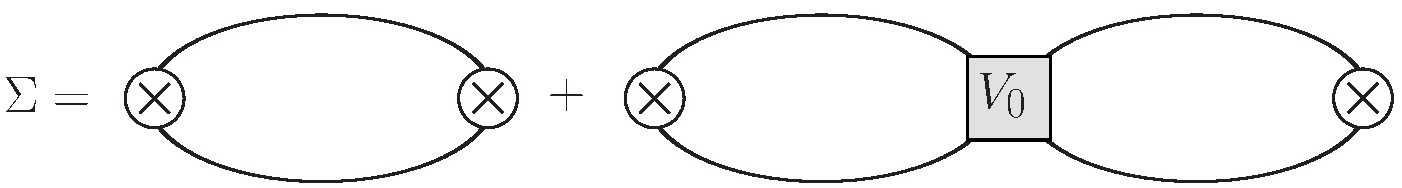
\includegraphics[width=0.5\textwidth]{figs/LO_NLO_Self_Energy.pdf}
\caption{The deuteron self-energy up to NLO.}
\end{figure}

\begin{figure}[ht]
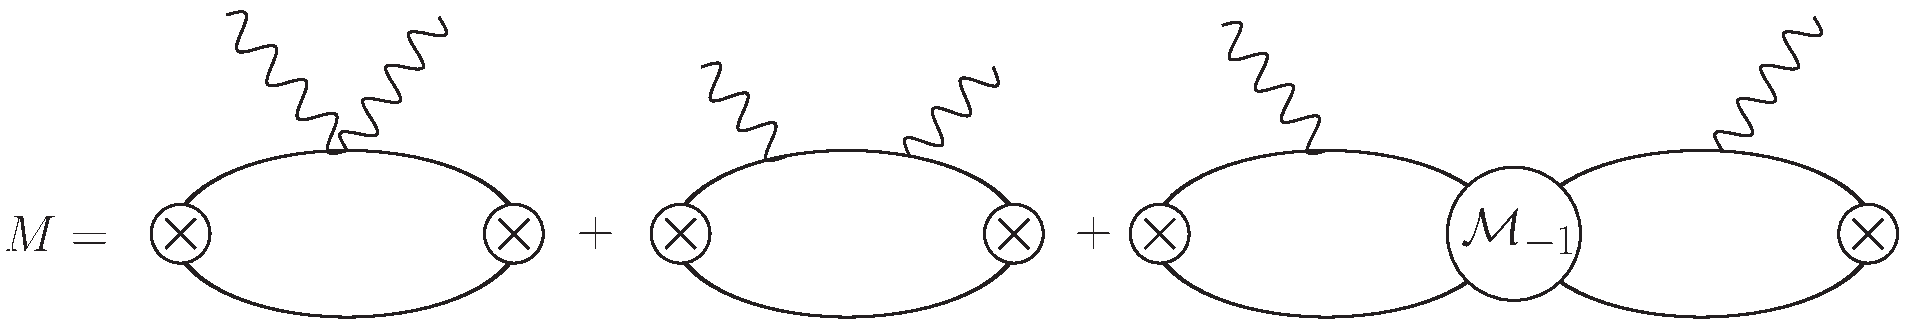
\includegraphics[width=0.75\textwidth]{figs/LO_VVCS_Diagrams.pdf}
\caption{Deuteron VVCS graphs contributing to $f_L$ at LO.}
\end{figure}

\begin{figure}[htb]
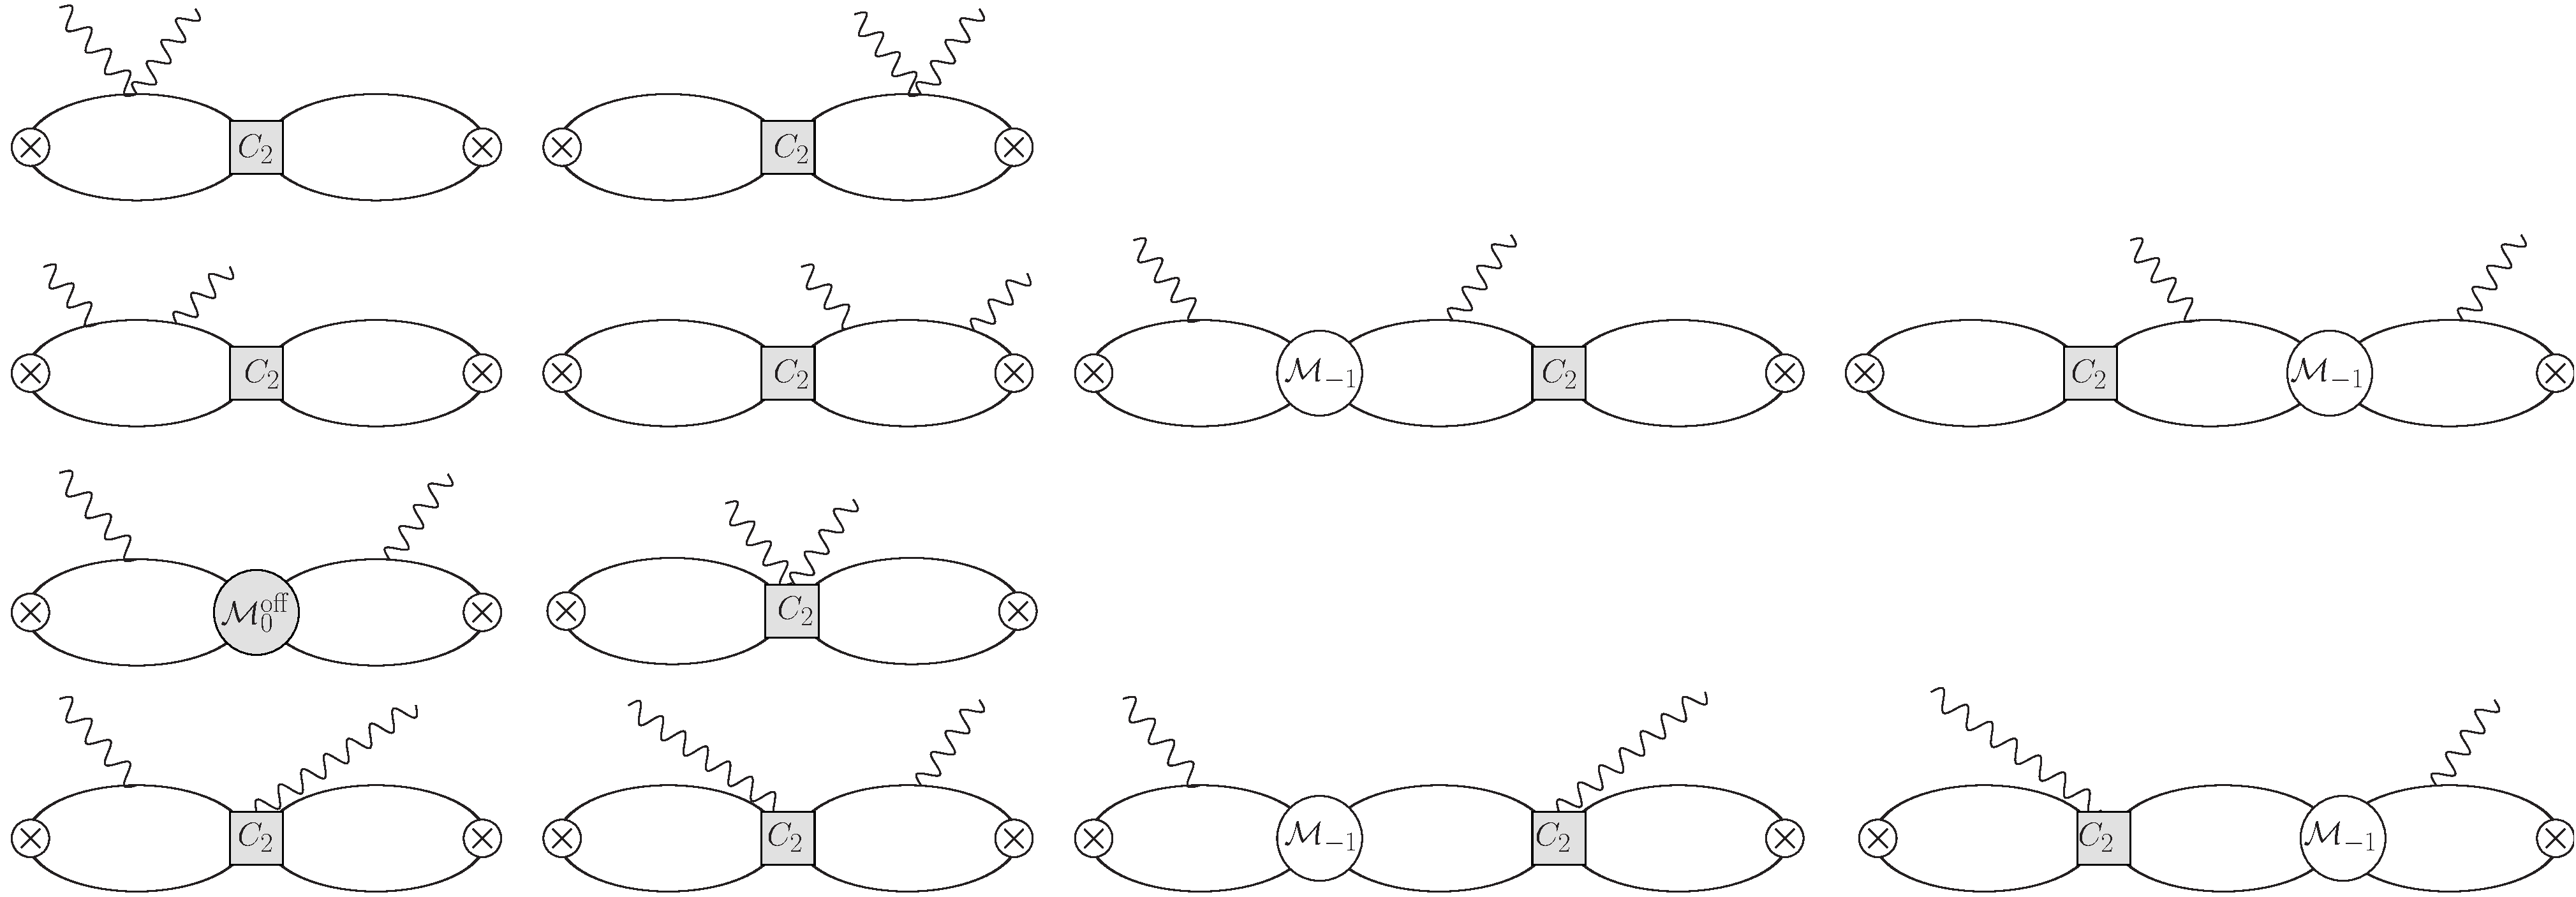
\includegraphics[width=\textwidth]{figs/NLO_VVCS_Diagrams.pdf}
\caption{Deuteron VVCS graphs contributing to $f_L$ at NLO.}
\end{figure}

\begin{figure}[htb]
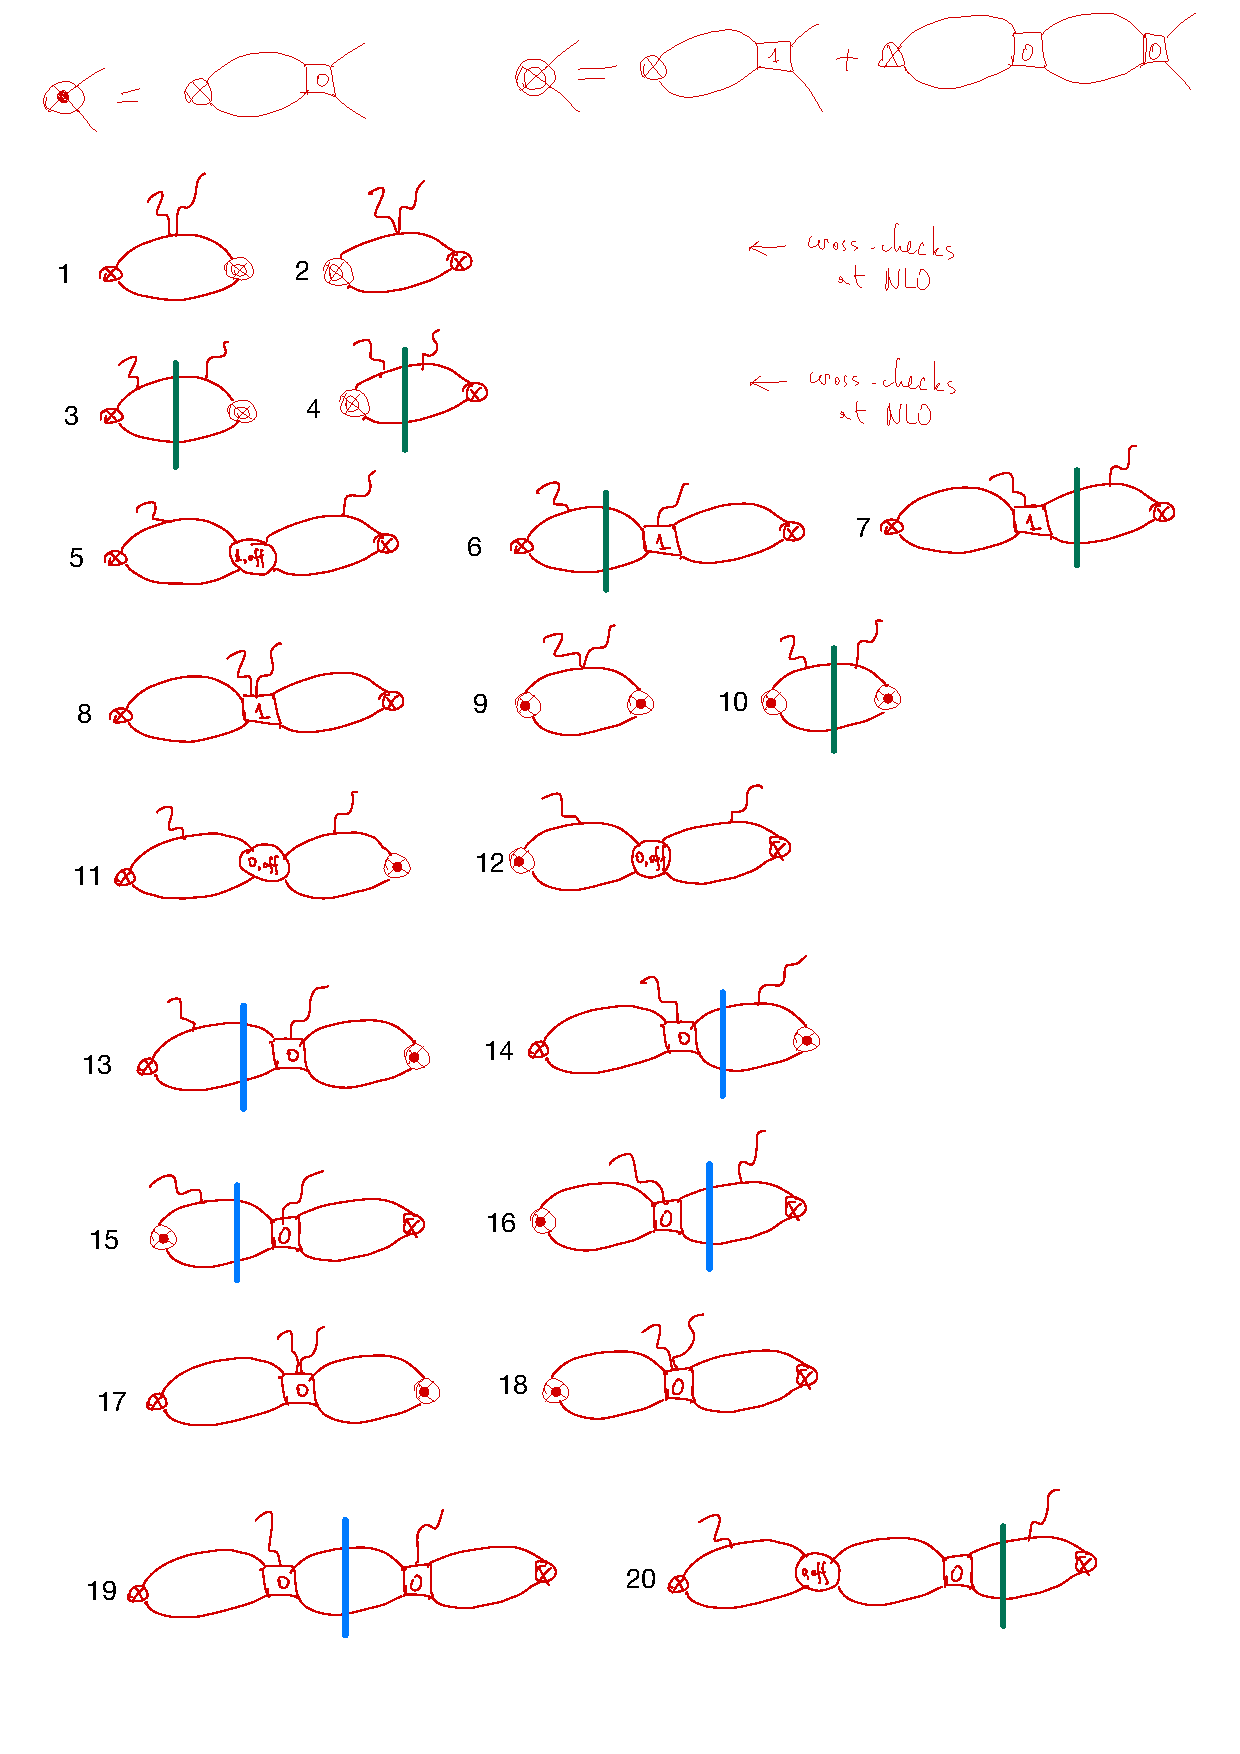
\includegraphics[width=\textwidth]{figs/N2LO.pdf}
\caption{Deuteron VVCS graphs contributing to $f_L$ at NNLO. Green vertical lines denote a possible insertion of $\mathcal{M}_{-1}^{t}$. Blue vertical lines denote possible insertions of $\mathcal{M}_{-1}^{t}$ that vanish due to isospin.}
\end{figure}

\section{TPE contribution to the Lamb shift}

\begin{align}
\Delta E_{2S}&=
\frac{\alpha}{2\pi^2 m_\mu}\phi_{2S}(0)^2
\int \mathrm{d}^4 q
\frac{f_L(-iq_0,Q^2)-2(q_0^2/Q^2) f_T(-iq_0,Q^2)}{Q^2
\left(\frac{Q^4}{4m_\mu^2}+q_0^2\right)}\\
&=\frac{2\alpha}{\pi m_\mu}\phi_{2S}(0)^2
\int\limits_0^\infty\frac{\mathrm{d}Q}{Q}\int\limits_{-1}^{1} \mathrm{d}x\,\sqrt{1-x^2}\,
\frac{f_L(-iQx,Q^2)-2x^2 f_T(-iQx,Q^2)}{
\frac{Q^2}{4m_\mu^2}+x^2}.
\end{align}
The normalization of the amplitude is
\begin{align}
    f_L(\nu,Q^2) = \alpha_{E1}Q^2 +\dots\,.
\end{align}

The contribution comes predominantly from the longitudinal amplitude, see Table~\ref{tab:resultsorders}. The transverse amplitude contribution starts at N4LO in the counting, and the numerical calculation confirms its smallness, giving $-0.003$~meV (taking LO+NLO for $f_T$).

\begin{table}[hbt]
\label{tab:resultsorders}
\begin{tabular}{c||c c c || c}
                         & LO       & NLO       & NNLO     & Total\\
\hline
\hline
$\Delta E_{2S}$ [meV]    & $-0.944$ & $-0.634$  & $\hpm 0.010$  & $-1.568$    
\end{tabular}
\caption{Results for the inelastic TPE contribution}
\end{table}

\section{Discussion}

\newpage
\appendix
\section{VVCS amplitude}
Here, we give analytic expressions for the longitudinal VVCS amplitude $f_L(\nu,Q^2)$.
\paragraph{LO}

\begin{align}
 f_L(\nu,Q^2)& = \frac{4 e^2 m Q^2}{q^4} \left(\frac{q^2}{4 (\gamma +\lambda_\mathrm{d})^2+q^2}-\frac{2 \gamma  \arctan\left[\frac{q}{2 (\gamma +\lambda_\mathrm{d})}\right]^2}{\gamma -\lambda_\mathrm{d}}-\frac{16 \gamma ^2 \arctan\left[\frac{q}{4 \gamma }\right]^2}{q^2-4 m \nu }\right)\nonumber\\
   & + (\nu\to-\nu)\,,
\end{align}
where $q=\sqrt{Q^2+\nu^2}$ is the photon three-momentum, and $\lambda_d=\sqrt{\gamma^2-m\nu+q^2/4}$. In practice, one can directly replace $q\to Q$ (which is consistent with the non-relativistic counting at least up to NLO). The numerical effect due to that change is very small.

\section{Conversion between observables}

The structure functions are directly related to the imaginary parts of the VVCS amplitudes $W\equiv\Im(\mathcal{M})$:
\begin{align}
F_1=&\frac{W_{TL}+2W_{TT}}{3}\\
F_2=&\frac{Q^2}{3(\nu^2+Q^2)}\left(W_{TL}+2W_{TT}+W_{LL}+2W_{LT}\right)\\
g_1=&\frac{\nu}{\nu^2+Q^2}\left(\sqrt{Q^2}W_{TL}^a-\nu W_{TT}^a\right)\\
g_2=&\frac{\nu^2}{\nu^2+Q^2}\left(\frac{\nu}{\sqrt{Q^2}}W_{TL}^a+W_{TT}^a\right)\\
b_1=&W_{TL}-W_{TT}\\
b_2=&\frac{Q^2}{\nu^2+Q^2}\left(W_{TL}-W_{TT}+W_{LL}-W_{LT}\right)\\
b_3=&\frac{\nu^2}{\sqrt{Q^2(\nu^2+Q^2)}}W_{TL}^\tau\\
\Delta=&W_{TT}^\tau,\\
\intertext{
or the inverse relations}
W_{TL}^a=&\frac{\sqrt{Q^2}}{\nu}(g_1+g_2)\\
W_{TT}^a=&\frac{Q^2}{\nu^2}g_2-g_1\\
W_{TT}^\tau=&\Delta\\
W_{TL}^\tau=&\frac{\sqrt{Q^2(\nu^2+Q^2)}}{\nu^2}b_3\\
W_{TT}=&F_1-\frac{b_1}{3}\\
W_{TL}=&F_1+\frac{2b_1}{3}\\
W_{LT}=&-F_1+\frac{b_1}{3}+\frac{\nu^2+Q^2}{Q^2}\left(F_2-\frac{b_2}{3}\right)\\
W_{LL}=&-F_1-\frac{2b_1}{3}+\frac{\nu^2+Q^2}{Q^2}\left(F_2+\frac{2b_2}{3}\right).
\end{align}
%
Furthermore, the cross-sections of light-by-light scattering are related to the VVCS amplitudes as
%
\begin{align}
W_{TT} &= 2\sqrt{X}\sigma_{TT} 
\\
W_{TT}^\tau &= 2\sqrt{X}\tau_{TT}\\
W_{TT}^a &= 2\sqrt{X}\tau_{TT}^a\\
W_{TL} &= 2\sqrt{X}\sigma_{TL}\\
W_{LT}  &= 2\sqrt{X}\sigma_{LT}\\
W_{LL}  &= 2\sqrt{X}\sigma_{LL}\\
W_{TL}^\tau &= 2\sqrt{X}\tau_{TL}\\ W_{TL}^a &= 2\sqrt{X}\tau_{TL}^a,
\end{align}
where $X\equiv(p\cdot q)^2-M^2q^2$.


\section{Lagrangians and counting}
\subsection{One-nucleon Lagrangian}
Hill et al.~\cite{Hill:2012rh} write down the following non-relativistic one-nucleon
Lagrangian up to $1/M^4$:
\begin{align}
\mathcal{L} &= \psi^\dagger
  \bigg\{  i D_t  + c_2 \frac{\bm{D}^2 }{ 2M}  + c_4 \frac{\bm{D}^4 }{ 8 M^3} +
  c_F g\frac{ \bm{\sigma}\cdot \bm{B} }{ 2M}   
+ c_D g\frac{ [\bm{\partial}\cdot \bm{E}] }{ 8 M^2}  
+ i c_S g\frac{ \bm{\sigma} \cdot ( \bm{D} \times \bm{E} - \bm{E}\times \bm{D} ) }{ 8 M^2} 
\nn\\
&\quad
+ c_{W1}g \frac{  \{ \bm{D}^2 ,  \bm{\sigma}\cdot \bm{B} \}  }{ 8 M^3}  
- c_{W2}g \frac{  D^i \bm{\sigma}\cdot
    \bm{B} D^i }{ 4 M^3 }  + c_{p^\prime p} g \frac{ \bm{\sigma} \cdot
    \bm{D} \bm{B}\cdot \bm{D} + \bm{D}\cdot\bm{B} \bm{\sigma}\cdot \bm{D}
    }{  8 M^3} 
\nn\\
&\quad 
+ i c_M g \frac{ \{ \bm{D}^i ,  [\bm{\partial} \times \bm{B}]^i \} }{ 8 M^3}
+ c_{A1} g^2\frac{ \bm{B}^2 - \bm{E}^2 }{ 8 M^3}  - c_{A2} g^2\frac{ \bm{E}^2 }{ 16 M^3 } 
\nn \\
&\quad 
+ c_{X1}g \frac{ [ \bm{D}^2 , \bm{D}\cdot \bm{E} + \bm{E}\cdot\bm{D} ] }{ M^4 }
+ c_{X2}g \frac{ \{ \bm{D}^2 , [\bm{\partial}\cdot\bm{E}] \} }{ M^4 }
+ c_{X3}g \frac{ [\bm{\partial}^2 \bm{\partial}\cdot\bm{E}] }{ M^4 } 
\nn \\
&\quad 
+ i c_{X4}g^2 \frac{ \{ \bm{D}^i , [\bm{E}\times\bm{B}]^i \} }{ M^4 } 
+ ic_{X5} g \frac{ D^i \bm{\sigma}\cdot ( \bm{D}\times\bm{E} - \bm{E}\times\bm{D} )D^i   }{ M^4} 
+ ic_{X6} g \frac{ \epsilon^{ijk} \sigma^i D^j [\bm{\partial}\cdot\bm{E}] D^k }{ M^4} 
\nn \\
&\quad
+ c_{X7} g^2 \frac{ \bm{\sigma}\cdot\bm{B} [\bm{\partial}\cdot\bm{E}] }{ M^4} 
+ c_{X8} g^2 \frac{ [\bm{E}\cdot\bm{\partial} \bm{\sigma}\cdot\bm{B} ] }{ M^4}
+ c_{X9} g^2 \frac{ [\bm{B}\cdot\bm{\partial} \bm{\sigma}\cdot\bm{E} ] }{ M^4} 
+ c_{X10} g^2 \frac{ [E^i \bm{\sigma}\cdot\bm{\partial} B^i] }{ M^4}
\nn \\
&\quad
+ c_{X11} g^2 \frac{ [B^i \bm{\sigma}\cdot\bm{\partial} E^i]}{M^4} 
+ c_{X12} g^2 \frac{ \bm{\sigma}\cdot \bm{E}\times [{\partial_t}\bm{E}-\bm{\partial}\times\bm{B} ] }{ M^4}
+ \mathcal{O}(1/M^5)
 \bigg\} \psi  \,.
 \label{eq:abelian}
 \end{align}
In this equation, $D_t=\partial_t + i g Z A_0$, $\vec D=\vec\nabla - i g Z \vec A$.
We assume that $g=+1$ for the proton (which is consistent with papers such as, e.g., \cite{Dye:2016uep},
and also with, for instance, the $\bm{\sigma}\cdot\bm{B}$ term entering with the positive sign in the Lagrangian, so that the corresponding term in the Hamiltonian is $-\bm{\mu}\cdot\bm{B}$).
For our purposes, we only need terms up to $1/M^3$. Setting $g=1$ gives
\begin{align}
\mathcal{L} &= \psi^\dagger
  \bigg\{  i D_t  + c_2 \frac{\bm{D}^2 }{ 2M}  + c_4 \frac{\bm{D}^4 }{ 8 M^3} +
  c_F \frac{ \bm{\sigma}\cdot \bm{B} }{ 2M}   
+ c_D \frac{ [\bm{\partial}\cdot \bm{E}] }{ 8 M^2}  
+ i c_S \frac{ \bm{\sigma} \cdot ( \bm{D} \times \bm{E} - \bm{E}\times \bm{D} ) }{ 8 M^2} 
\nn\\
&\quad
+ c_{W1} \frac{  \{ \bm{D}^2 ,  \bm{\sigma}\cdot \bm{B} \}  }{ 8 M^3}  
- c_{W2} \frac{  D^i \bm{\sigma}\cdot
    \bm{B} D^i }{ 4 M^3 }  + c_{p^\prime p}  \frac{ \bm{\sigma} \cdot
    \bm{D} \bm{B}\cdot \bm{D} + \bm{D}\cdot\bm{B} \bm{\sigma}\cdot \bm{D}
    }{  8 M^3} 
\nn\\
&\quad 
+ i c_M  \frac{ \{ \bm{D}^i ,  [\bm{\partial} \times \bm{B}]^i \} }{ 8 M^3}
+ c_{A1} \frac{ \bm{B}^2 - \bm{E}^2 }{ 8 M^3}  - c_{A2} \frac{ \bm{E}^2 }{ 16 M^3 } 
+ \mathcal{O}(1/M^4)
 \bigg\} \psi  \,.
 \label{eq:abelian3}
 \end{align}
 The constants entering the Lagrangian are given by Hill et al.\ as
 \begin{align}
     c_2 = 1,\quad  c_S = 2 c_F - Z,\quad  c_4 = 1,\quad 2 c_M = c_D - c_F,\quad c_{W2} = c_{W1} - Z,\quad c_{p'p} = c_F - Z,
 \end{align}
 and the independent constants are obtained by matching (up to the possible radiative corrections) as
 \begin{align}
c_F = Z + \kappa,\quad c_D = Z + \frac{4}{3}M^2 \left\langle r_E^2\right\rangle,\quad 
c_{W1} = Z + \frac{1}{2}\kappa +\frac{2}{3}M^2\left\langle r_M^2\right\rangle \,,
 \end{align}
 where $r_E$ and $r_M$ are the nucleon charge and magnetic radii. Finally,
 \begin{align}
     c_{A1} = Z^2 + \frac{4M^3}{\alpha_\mathrm{em}}\beta_{M1},\quad c_{A2} = 2\kappa^2 +\frac{8Z}{3}M^2 \left\langle r_E^2\right\rangle -\frac{8M^3}{\alpha_\mathrm{em}}(\alpha_{E1}+\beta_{M1}).
 \end{align}
This gives
\begin{align}
\mathcal{L} &= \psi^\dagger
  \bigg\{  i D_t  + \frac{\bm{D}^2 }{ 2M}  +  \frac{\bm{D}^4 }{ 8 M^3} +
  \mu \frac{ \bm{\sigma}\cdot \bm{B} }{ 2M}   
+ \left(Z + \frac{4}{3}M^2 \left\langle r_E^2\right\rangle\right)\frac{ [\bm{\partial}\cdot \bm{E}] }{ 8 M^2}  
+ i \left(\mu-\frac{Z}{2}\right) \frac{ \bm{\sigma} \cdot ( \bm{D} \times \bm{E} - \bm{E}\times \bm{D} ) }{ 4 M^2} 
\nn\\
&\quad
+ c_{W1} \frac{  \{ \bm{D}^2 ,  \bm{\sigma}\cdot \bm{B} \}  }{ 8 M^3}  
- c_{W2} \frac{  D^i \bm{\sigma}\cdot
    \bm{B} D^i }{ 4 M^3 }  + c_{p^\prime p}  \frac{ \bm{\sigma} \cdot
    \bm{D}\ \bm{B}\cdot \bm{D} + \bm{D}\cdot\bm{B}\ \bm{\sigma}\cdot \bm{D}
    }{  8 M^3} 
\nn\\
&\quad 
+ i c_M  \frac{ \{ \bm{D}^i ,  [\bm{\partial} \times \bm{B}]^i \} }{ 8 M^3}
+ c_{A1} \frac{ \bm{B}^2 - \bm{E}^2 }{ 8 M^3}  - c_{A2} \frac{ \bm{E}^2 }{ 16 M^3 } 
+ \mathcal{O}(1/M^4)
 \bigg\} \psi  \,.
 \label{eq:abelian3c}
 \end{align}
 Note that species-dependent numbers such as $Z$, $\kappa$, and so on, have to be replaced by
 the corresponding isospin-dependent operators.
\subsection{Notes on the counting}
One could consider a counting scheme where both parts entering $D_0=\partial_0+i e A_0$ would
count as $O(p^2)=O(ep)$.
This, however, is not consistent with the LEX of $f_L=Q^2\alpha_{E1} + \omega^2 Q^2\alpha_L + \dots$;
since $\alpha_{E1}=O(e^2p^{-4})$, $f_L=O(e^2p^{-2})$. The counting of the corresponding loop,
containing two insertions of the $A_0$ interaction, would give $f_L=O(e^2p^{1+2+5-8=0})$.
This means that $A_0$ should be counted as $O(p^0)$. The one-loop amplitude thus contains different
orders.


\section{Calculation}

\subsection{Leading order}

\subsection{Next-to-leading order}

\subsection{Relativistic}
\begin{align}
    &\sigma_L(s,Q^2)=
    \frac{e^2 g^2 Q^2}
        {144 \pi  \left(M^2-s\right)^4
        \left(2 M^2\left(Q^2-s\right)+M^4+\left(Q^2+s\right)^2\right)
        }\nonumber\\
   &\times
   \Bigg\{
   \frac{
        v\lambda
        }
            {M^2 s \left(M^2 \left(2 m^2 \left(Q^2-s\right)-Q^2 s\right)+m^2 M^4+m^2\left(Q^2+s\right)^2\right)
        }\nonumber\\
   &\times
   \Bigg[s^6 \left(M^2 \left(38m^2-Q^2\right)+2 m^2 \left(m^2+Q^2\right)\right)\nonumber\\
   &+s^5 \Big(M^4 \left(31 m^2-40 Q^2\right)+4 M^2 \left(31 m^2 Q^2+43 m^4\right)+m^2 Q^2 \left(4 m^2-Q^2\right)+48M^6\Big)\nonumber\\
   &-2 s^4 \Big(M^6 \left(22 m^2+7 Q^2\right)+M^4 \left(86 m^2 Q^2+65 m^4+22 Q^4\right)-M^2 Q^2 \left(62 m^2 Q^2+222 m^4+Q^4\right)\nonumber\\
   &+m^2 Q^4 \left(m^2+2Q^2\right)+48 M^8\Big)\nonumber\\
   &+s^3 \Big(-M^8 \left(161 m^2+136 Q^2\right)+8 M^6 \left(20 m^2 Q^2-35 m^4+2 Q^4\right)+2 M^4 Q^2 \left(m^2 Q^2+292 m^4+4 Q^4\right)\nonumber\\
   &+8 m^2 M^2 Q^4 \left(43 m^2+4 Q^2\right)-m^2 Q^6 \left(8 m^2+Q^2\right)+48 M^{10}\Big)\nonumber\\
   &-s^2 \left(M^2+Q^2\right)^2 \Big(M^6 \left(Q^2-134 m^2\right)+2 M^4 \left(m^2 Q^2-127 m^4+Q^4\right)+M^2 Q^2 \left(6 m^2 Q^2\right.\nonumber\\
   &\left.-60 m^4+Q^4\right)+2 m^2 Q^4 \left(m^2-Q^2\right)\Big)\nonumber\\
   &+m^2 s \left(M^2+Q^2\right)^4 \left(-20 m^2 M^2+Q^2 \left(4
   m^2+Q^2\right)+M^4\right)+2 m^4 \left(M^2+Q^2\right)^6+m^2 s^7\Bigg]\nonumber\\
   &+48 \left(M^2-s\right) \left(M^2 \left(2 m^2 \left(Q^2+2 s\right)+s \left(s-Q^2\right)\right)+M^4 \left(m^2+3 s\right)+m^2
   \left(Q^2+s\right) \left(Q^2+3 s\right)\right) \nonumber\times\\
   &\log \left(\frac{\beta_\gamma+v\lambda}{\beta_\gamma-v\lambda}\right)\Bigg\},\\
   \intertext{where}
   %%
   &\lim_{s\rightarrow\infty}\sigma_L(s,Q^2)\rightarrow e^2g^2\frac{Q^2}{144\pi M^2s},\\
   %
   %
   &\sigma_T(s,Q^2)=\frac{e^2 g^2 Q^2}{144 \pi  \left(M^2-s\right)^4 \left(2 M^2
   \left(Q^2-s\right)+M^4+\left(Q^2+s\right)^2\right)}\nonumber\\
   &\Bigg\{-\frac{v\lambda}{M^2 s \left(M^2 \left(2 m^2 \left(Q^2-s\right)-Q^2 s\right)+m^2 M^4+m^2
   \left(Q^2+s\right)^2\right)}\nonumber\\
   &\times\Bigg[s^6 \left(M^2 \left(38
   m^2-Q^2\right)+2 m^2 \left(m^2+Q^2\right)\right)\nonumber\\
   &+s^5 \left(M^4 \left(31 m^2-40 Q^2\right)+4 M^2 \left(31 m^2 Q^2+43 m^4\right)+m^2 Q^2 \left(4 m^2-Q^2\right)+48
   M^6\right)\nonumber\\
   &-2 s^4 \Big(M^6 \left(22 m^2+7 Q^2\right)+M^4 \left(86 m^2 Q^2+65 m^4+22 Q^4\right)-M^2 Q^2 \left(62 m^2 Q^2+222 m^4+Q^4\right)\nonumber\\
   &+m^2 Q^4 \left(m^2+2
   Q^2\right)+48 M^8\Big)\nonumber\\
   &+s^3 \Big(-M^8 \left(161 m^2+136 Q^2\right)+8 M^6 \left(20 m^2 Q^2-35 m^4+2 Q^4\right)+2 M^4 Q^2 \left(m^2 Q^2+292 m^4+4 Q^4\right)\nonumber\\
   &+8 m^2
   M^2 Q^4 \left(43 m^2+4 Q^2\right)-m^2 Q^6 \left(8 m^2+Q^2\right)+48 M^{10}\Big)\nonumber\\
   &-s^2 \left(M^2+Q^2\right)^2 \Big(M^6 \left(Q^2-134 m^2\right)+2 M^4 \left(m^2
   Q^2-127 m^4+Q^4\right)+M^2 Q^2 \left(6 m^2 Q^2-60 m^4+Q^4\right)\nonumber\\
   &+2 m^2 Q^4 \left(m^2-Q^2\right)\Big)\nonumber\\
   &+m^2 s \left(M^2+Q^2\right)^4 \left(-20 m^2 M^2+Q^2 \left(4
   m^2+Q^2\right)+M^4\right)+2 m^4 \left(M^2+Q^2\right)^6+m^2 s^7\Bigg]\nonumber\\
   &-48 \left(M^2-s\right) \left(M^2 \left(2 m^2 \left(Q^2+2 s\right)+s \left(s-Q^2\right)\right)+M^4 \left(m^2+3 s\right)+m^2
   \left(Q^2+s\right) \left(Q^2+3 s\right)\right)\nonumber\\
   &\times \log \left(\frac{\beta_\gamma+v\lambda}{\beta_\gamma-v\lambda}\right)\Bigg\}
\end{align}

\bea
\be_D &=& \frac{s+M^2-Q^2}{2s} ,\\
\be_\ga &=& \frac{s-M^2+Q^2}{2s}, \\
v &=& \sqrt{1- \frac{4m^2}{s}},\\
\la &=& \frac{1}{2s} \sqrt{\big[Q^2 +(\sqrt{s} +M) ^2 \big]
\, \big[Q^2 +(\sqrt{s} -M) ^2 \big]}
\eea

\beq 
\log \frac{ \beta_\ga + v\la }{\beta_\ga - v\la }
\eeq
\section{Results and discussion}

\section{Off-forward corrections, notes}
We want to calculate the $t$-channel cut discontinuity of the box diagram:
\begin{align}
    M=-i\int\frac{\mathrm{d}^4 q}{(2\pi)^4}\frac{L_{\mu\nu}T^{\mu\nu}}{q^2q^{\prime\,2}}\,,
\end{align}
where $L_{\mu\nu}$ is the lepton Compton tensor, $T^{\mu\nu} = T^{\mu\nu}(q^2,q^{\prime\,2},\nu,t)$
is the nuclear VVCS amplitude, and $q' = q + p - p'$.

Using the Cutkosky rules gives
\begin{align}
    \Disc M = -i\int\frac{\mathrm{d}^4 q}{(2\pi)^4}L_{\mu\nu}T^{\mu\nu}(-2\pi i)^2\delta(q^2)\delta(q^{\prime\,2})=\frac{i}{(2\pi)^2}\int\mathrm{d}^4 q\, L_{\mu\nu}T^{\mu\nu}\delta(q^2)\delta(q^{\prime\,2})\,,
\end{align}

\section{Whatever comes here}

\section{VVCS tensor basis}

\section{Feynman rules}
\subsection{One-nucleon Lagrangian}
\subsubsection{Nucleon propagator}
\begin{align}
    iG(E,\vec p\,) = \frac{i}{E-\frac{p^2}{2M}+i0}
\end{align}
\subsubsection{$1/M^2$ correction to the nucleon propagator}
\begin{align}
    i\Gamma = 
\end{align}
\subsubsection{$\gamma NN$ vertex}
The terms are ordered in the $1/M$ expansion. The photon momentum is incoming in the vertex
(so that $\vec p^{\,\prime} = \vec p + \vec q\,$). Furthermore,
\begin{align}
    \hat{Q} = \frac{1}{2}(1+\tau_3)\,,\qquad \hat{\mu} = \mu_s +\mu_v\tau_3\,
\end{align}
with $\mu_{s,v}=(\mu_p\pm\mu_n)/2$.
\begin{align}
i\Gamma(\omega, \vec q,\vec p\,) = 
\end{align}

\subsubsection{$\gamma\gamma NN$ vertex}
\begin{align}
    i\Gamma(\omega, \vec q,\omega',\vec q^{\,\prime},\vec p\,)&= -\frac{ie^2}{M}\hat{Q}\, \ve\cdot\vep \nn\\
    & +\frac{e^2}{2M^2}\hat{Q}\left(\mu_p+\frac{1}{2}\right)\vec\sigma\cdot\left[\ve\times\vep(\omega+\omega')+(\ezp\, \vec q^{\,\prime} \times\ve -\ez \, \vec q\times\vep)\right]
\end{align}
\subsection{Two-nucleon Lagrangian}
\subsubsection{$NN$ interaction}
\subsubsection{$\gamma NNNN$ contact terms}
\subsubsection{$\gamma \gamma NNNN$ contact terms}

\subsection{Some integrals}
\begin{align}
  \mathrm{i}\int\frac{\mathrm{d}^4 \ell }{(2\pi)^4}\frac{(\vec \ell-\vec p/2)^{2n}}{\left[\ell_0-\frac{\vec\ell^2}{2M}+\mathrm{i}0\right]\left[E-\ell_0-\frac{(\vec\ell-\vec p)^2}{2M}+\mathrm{i}0\right]}\equiv I_n(\bar{E})= -\frac{M}{4\pi}\left(M \bar{E}\right)^n\left(\mu -\sqrt{-M\bar{E}-\mathrm{i}0}\right)\,,
\end{align}
where $\bar{E}=E-\vec p^{\,2}/4M$.

\bibliography{pionless_eft}
\end{document}
